\documentclass[pdftex,12pt,oneside,openany,a4paper]{book}
\usepackage[brazilian]{babel}
\usepackage[utf8]{inputenc} % Aqui tem que mudar de acordo com o seu sistema operacional
\usepackage[T1]{fontenc} %
\usepackage[pdftex]{graphicx} % includegraphics
\usepackage{subfigure} % Poder colocar varias figuras juntas
\usepackage[unicode]{hyperref} % Para adicionar os links no pdf
\usepackage[all]{hypcap}
\usepackage{array} % Adicionar a opcao m e b em tabelas e um monte de coisa que eu nao usei
\usepackage[overload]{textcase} % Adicionar MakeUpperCase etc.
\usepackage{rotating} % Para rodar as figuras e tabelas
\usepackage{pdflscape} % Para colocar paginas na horizontal no pdf
\usepackage{eurosym} % Para o simbulo de Euro
\usepackage{amssymb} % Para adicionar um monte de simbolos que nao existem normalmente, 
  % como aproximadamente menor que.
\usepackage{ccaption} % Para footnotes dentro de captions
\hypersetup{
    unicode=true,          % non-Latin characters in Acrobat’s bookmarks
    pdftitle={Projeto Final},    % title
    pdfauthor={Werner Spolidoro Freund},     % author
    pdfsubject={Projeto Final},   % subject of the document
    colorlinks=true,       % false: boxed links; true: colored links
    pdfdisplaydoctitle=true,
    citecolor=black,%
    filecolor=black,%
    linkcolor=black,%
    urlcolor=black%
}

\usepackage{indentfirst} % Para dar espaço para o primeiro parágrafo
\usepackage{multirow} % Tabelas com celulas agrupadas
\usepackage{amsmath}  % equation etc
\usepackage{listings} % Para colocar códigos de programas
%\usepackage{simplemargins}
% Formato do PF
\usepackage{layout} 
% Modelo da página
\setlength{\textheight}{24.7cm}
\setlength{\textwidth}{15cm}
\setlength{\footskip}{1.25cm}
\setlength{\footnotesep}{0.5cm}
\setlength{\headheight}{0pt}
\setlength{\headsep}{0pt}
\setlength{\oddsidemargin}{0.46cm} % 0.46
\setlength{\topmargin}{-.04cm}   %-.04
\setlength{\marginparsep}{0pt}
\setlength{\marginparwidth}{0pt}
\setlength{\parindent}{1.25cm}
\renewcommand{\baselinestretch}{1.5}
\pagestyle{plain}

%\usepackage[style=long,nonumberlist,toc]{glossaries}
\usepackage[style=long,nonumberlist,sanitize=none]{glossaries} % Para as listas de simbolos e abreviaturas
\renewcommand{\glossaryname}{S{í}mbolos e Abreviaturas}
%\renewcommand{\glossarypreamble}{Texto principal}
% Define a new glossary type
\newglossary[slg]{Simb}{sym}{sbl}{Lista de S{í}mbolos}
\newglossary[alg]{Abrev}{abr}{abv}{Lista de Abreviaturas}

\makeglossaries

% add = sign in the list of abbreviations:

\renewenvironment{theglossary}
  {\begin{longtable}{l@{{ }{ }{ }{ }{ }{ }{ }{ }{ }{ }}p{0.80\textwidth}}}
  {\end{longtable}}%
\renewcommand{\glsgroupskip}{}


%\renewcommand{\contentsname}{Whatever}
\setcounter{secnumdepth}{4}
\setcounter{tocdepth}{4}
%\makeatletter
%\renewcommand\paragraph{%
%  \@startsection{paragraph}{4}{0mm}%
%    {-\baselineskip}%
%    {.5\baselineskip}%
%    {\normalfont\normalsize\bfseries}}
%\makeatother
\makeatletter
\renewcommand\paragraph{\@startsection{paragraph}{4}{\z@}%
    {-3.25ex\@plus -1ex \@minus -.2ex}%
    {1.5ex \@plus .2ex}%
    {\normalfont\normalsize\bfseries}}
\makeatother

\newcommand*{\fnref}[1]{\textsuperscript{\ref{#1}}}
%\newcommand*{\addtotoc}[2]{\clearpage\phantomsection\addcontentsline{toc}{#1}{#2}}

\begin{document}

\begin{titlepage}
	\vfill
	\begin{center}
		{\large \uppercase{\bf{Algoritmo Alternativo utilizando informação anelada de calorimetria para discriminação de elétrons/fótons para o detector ATLAS}}}\\[0.9cm]
    {Werner Spolidoro Freund}\\[0.9cm]
  \end{center}

		{\uppercase{PROJETO SUBMETIDO AO CORPO DOCENTE DO DEPARTAMENTO DE ENGENHARIA ELÉTRICA DA ESCOLA POLITÉCNICA DA UNIVERSIDADE FEDERAL DO RIO DE JANEIRO COMO PARTE DOS REQUISITOS NECESSÁRIOS PARA A OBTENÇÃO DO GRAU DE ENGENHEIRO ELETRICISTA.}}\\[0.3cm]

    {Aprovada por:}\\[0.5cm]

  \begin{flushright}
		\begin{tabular}{lr}
			{\bf Orientador:} & \rule{8cm}{0.4pt} \\
					 & Carmem Lúcia Tancredo Borges, D.Sc. \\[0.5cm]
			{\bf Coorientador:}& \rule{8cm}{0.4pt} \\ 
					 & José Manoel de Seixas, D.Sc. \\[0.5cm]
			{\bf Examinador:}& \rule{8cm}{0.4pt} \\
					 & Caloba, D.Sc. \\[0.5cm]
			{\bf Examinador:}& \rule{8cm}{0.4pt} \\
					 & Carmem do lps, M.Sc. \\[0.5cm]
			{\bf Examinador:}& \rule{8cm}{0.4pt} \\
					 & Mais alguem do DEE (Lopes?), M.Sc. \\
		\end{tabular}
	\end{flushright}
    \vskip1.0cm
  \begin{center}
		\begin{large}
			RIO DE JANEIRO, RJ - BRASIL \\
      JULHO DE 2011
		\end{large}
  \end{center}
\end{titlepage}

\cleardoublepage

\null
\vfill
\begin{flushright}
  \em{Àqueles que buscam o conhecimento.}\\
\end{flushright}

\pagenumbering{roman}
% Agradecimento
\cleardoublepage

\begin{center}
\textbf{\Large Agradecimento}
\end{center}

Agradeço em primeiro lugar aos meus pais, Ronaldo e Cristina, 
pela educação e apoio que me deram. Aos meus irmãos que sempre
estiveram comigo, enriquecendo os bons momentos e me divertindo. Aos meus 
avôs Ronaldo e Gisela, por sempre terem me acolhido.

Aos meus orientadores R. Torres, D. Damazio, J. Seixas pelo conhecimento
transmitido, pelo incentivo que me deram, e pela paciência. Obrigado 
por terem acreditado e por tudo que fizeram por mim. Muito mais do que
orientadores, a presença de vocês sempre é agradável. Agradeço ao E. Simas pela
ajuda dada com o material e pela compreensão durante a época de sua tese com a
dificuldade de acertar os dados, nem sempre as coisas são tão simples quanto nós
queremos.

Também aos bons professores da elétrica que me ensinaram e trouxeram 
verdadeiros desafios a serem superados. Graças a vocês me sinto preparado para
qualquer dificuldade que venha a aparecer no futuro.
À Kátia, secretária da elétrica, que tem uma paciência sem fim para lidar com as
perguntas um tanto ou quanto repetitivas dos alunos, desde sua época de calouros
até a colação de grau. 

\newacronym[type=Abrev]{ufrj}{UFRJ}{Universidade Federal do Rio de Janeiro}
\newacronym[type=Abrev]{coppe}{COPPE}{instituto alberto luiz COimbra de
  Pós-graduação e Pesquisa de Engenharia}
\newacronym[type=Abrev]{lps}{LPS}{Laboratório de Processamento de Sinais -
 \acrshort{coppe}/\acrshort{ufrj}} 

Aos meus companheiros do \acrshort{lps}, D. Deva, D. Lima, 
dentre outros, pela contribuição e ajuda que me deram. Valhe destacar aqui que a
implementação inicial do código no Sistema de Reconstrução do Ringer foi feita pelo D. Lima
e ele em muito me auxiliou no entendimento do código complexo desse ambiente. 
Ainda, agradeço aos profissionais que nesse 
laboratório trabalham, principalmente a Talia, cuja dedicação se destaca.

Finalmente, agradeço a todos meus amigos que sempre me ajudaram quando precisei, 
eu lhes devo muito.

Muito obrigado a todos vocês!

\vfill
\begin{center}
\section*{Resumo\label{Resumo}}
\end{center}
\addcontentsline{toc}{chapter}{Resumo}

Ferramentas e tecnologias utilizadas em engenharia têm encontrado sua
aplicação em outras áreas do conhecimento.
Na Física, um dos ambientes que está no limiar da ciência atual é o maior acelerador 
de partículas já construído, o \acrshort{lhc}, que permitirá aos
cientistas validar e desenvolver teorias, como o \glslink{mp}{Modelo Padrão}. A
única partícula prevista ainda não observada por esse modelo é o bóson
de Higgs. Um dos detectores do \acrshort{lhc}, o \acrshort{atlas}, tem entre seus objetivos 
confirmar a existência de tal partícula. Todavia, o bóson de Higgs é altamente
instável, o que faz com que ele decaia rapidamente em outras partículas, como elétrons e fótons, de forma que é importante 
a detecção das mesmas para o sucesso do experimento. Por sua vez, essas
partículas têm sua assinatura mascarada por outras, como jatos hadrônicos, o que
torna o processo de sua identificação não trivial. 

O \gls{sr} do \acrshort{atlas} é o responsável por identificar as
partículas e seus parâmetros, assim capacidade de descoberta de novas físicas 
depende de sua eficiência. Outras dificuldades a serem superadas são a alta taxa de
eventos e a escassez dos eventos de interesse. 
O \gls{sf} foi desenvolvido para selecionar as informações relevantes para o experimento, 
atuando em tempo real, de forma a reduzir a grande quantidade de dados a ser armazenada.

Nesse contexto internacional, o presente trabalho realiza a continuação
do projeto \acrshort{egcaloringer}. O projeto consiste de um algoritmo 
para a identificação de elétrons e fótons, utilizando a informação especialista 
do detetor que é, então, propagada para um método estatístico de discriminação, 
atualmente formado por Redes Neurais, sendo uma das contribuições da
Engenharia para este experimento. O algoritmo de discriminação foi otimizado 
através do estudo do pré-processamento mais indicado para a rede neural. 
Embora o algoritmo tenha sido idealizado para o \gls{sf}, 
o mesmo foi portado por este trabalho ao \gls{sr}, de modo a permitir sua utilização e 
entendimento pela colaboração do \acrshort{atlas}. Sua performance foi 
testada utilizando como referência o algoritmo padrão utilizado 
pela colaboração. O algoritmo proposto superou o algoritmo padrão nas três bases
de dados testadas em relação à sua capacidade de discriminação.

\paragraph*{}

\noindent Palavra-chave: Redes Neurais, Sistema de Filtragem, Calorimetria.

\vfill

\clearpage

% Abstract
\vfill
\begin{center}
\section*{Abstract\label{Abstract}}
\end{center}
\addcontentsline{toc}{chapter}{Abstract}

Tools and technologies used in engineering have found their
application in other areas of expertise assisting on the Science evolutionary
process. In physics, one environment on Science's edge is the biggest
particle accelerator in the world, the \acrshort{lhc}, which will enable
scientists to validate and develop new theories, as the Standard Model. The only
particle not yet observed provided by this model is the Higgs boson. One of the LHC 
detectors, the ATLAS, has among its goals to confirm the existence
of this particle. The Higgs boson is highly unstable and will rapidly
decay in others particles, like electrons and photons, such that the detection
of those particles is important to the experiment triumph. These particles will 
have their signature faked by others such as hadronic jets, 
which makes the identification process not trivial.

The ATLAS Reconstruction System is responsible to identify the particles and its
parameters, therefore the discoverability of new physics is related to its
efficiency. Other difficulties that need to be overcome are the high event rate together
with events of interest scarcity. The Trigger System was developed to
select the relevant information for the experiment as an on-line algorithm in
order to reduce data storage.

In this international context, the present work proceed with the Egamma
Calorimeter project. The project consists of one algorithm to the 
ATLAS Reconstruction System, acting on the $e/\gamma$ physics channel. In this algorithm,
particular information from the detector is propagated to a stochastic
discrimination method, currently composed of Artificial Neural Networks, which
is one of the Engeneering contributions for this experiment.
This document describes the algorithm efficiency optimization through a study
of the most indicated data pre-processing. Furthermore, it was developed an
offline version for this algorithm, which was officially added to the ATLAS framework. 
The algorithm performance was tested using as benchmark the
standard algorithm developed by the collaboration. Finally, the proposed
algorithm overcomes the standart algorithm at the three datasets tested with
respect to their discrimination capacity.

\paragraph*{}

\noindent Key-words: neural networks, Trigger, Calorimetry.

\vfill
\clearpage

\cleardoublepage
% Sumário
\vfill
\clearpage \phantomsection \addcontentsline{toc}{chapter}{Sumário}
\tableofcontents
\clearpage \phantomsection \addcontentsline{toc}{section}{Lista de Figuras}
\listoffigures
\clearpage \phantomsection \addcontentsline{toc}{section}{Lista de Tabelas}
\listoftables
\clearpage \phantomsection \addcontentsline{toc}{section}{Lista de Símbolos}
%\renewcommand{\glossarypreamble}{Texto Simbulos}
\printglossary[type=Simb]
\clearpage \phantomsection \addcontentsline{toc}{section}{Lista de Abreviaturas}
\renewcommand{\glossarypreamble}{No caso de algumas abreviaturas
internacionalmente conhecidas, optou-se por mantê-las em sua lingua original.}
\printglossary[type=Abrev]
%\glssymbol{ohm}.

\cleardoublepage
\pagenumbering{arabic}

\chapter{Introdução}
\label{cap:intro}
\glsresetall

Varias áreas têm aplicações cuja alta taxa de eventos e a rara ocorrência de
eventos de interesse são uma dificuldade a ser superada. Técnicas de
Inteligência Computacional muitas vezes são utilizadas, como \acrlongpl{rna},
para reduzir, em tempo real, essa taxa a um nível adequado, selecionando eficientemente a
informação relevante ao experimento. Normalmente, se utilizam técnicas mais refinadas 
durante a análise a posteriori ao armazenamento dos dados, a fim de se obter
melhores resultados que aqueles realizados durante a análise em tempo real.

Em certos casos, a aplicação utiliza uma grande quantidade e diversidade de
sensores, sendo necessário o processamento dos sinais em uma informação mais
compacta, que possa representar com
fidelidade o fenômeno ocorrido. Novamente, as técnicas de Inteligência
Computacional e Processamento de Sinais Estocástico podem ser utilizadas para realizar a extração de
características, reduzindo o fluxo e quantidade de informação a ser analisada na aplicação.

%A engenharia tem auxiliado em diversas áreas através do emprego de
%novas tecnologias e o desenvolvimento de ferramentas que estão se tornando cada
%vez mais necessárias em áreas como medicina, biologia, ciências financeiras, etc. No caso de áreas
%multidisciplinares seu papel é ainda mais importante, quando ela e outras ciências 
%se aliam para caminhar juntas no desenvolvimento de ferramentas e tecnologias. 
%Com isso, se faz necessária a capacidade de sua adaptação à complexidade oferecida por esses novos ambientes, 
%como a alta quantidade e diversidade de sensores, alta taxa e raridade de
%eventos. Para realizar a interpretação dos diversos canais e a seleção dos eventos 
%de interesse, se faz mão de uma ferramenta que irá descartar a 
%informação inútil ao problema em questão, permanecendo apenas
%a parte necessária. É importante que ela seja eficiente para evitar a polarização
%dos eventos, onde a porção interessante dos mesmos seria desprezada.
%A tarefa se torna ainda mais difícil nos casos de 
%eventos raros de interesse, na qual a seleção errônea tem consequências piores,
%sendo necessário o emprego de técnicas para sua otimização. 
%
%O \glsdesc{sf}, a ferramenta citada, pode utilizar tanto de métodos baseados no conhecimento 
%especialista do assunto, quanto baseados na informação estatística do processo. Ainda, 
%a combinação do conhecimento especialista ao processamento estatístico trás uma abordagem ainda 
%mais poderosa através da utilização das informações em técnicas não lineares, 
%como \acrlongpl{rna}.
%
%A seleção de eventos pode ser realizada no ambiente em tempo real,
%quando o processo ocorre durante a aquisição de dados. Nesse
%ambiente, deseja-se reduzir o volume de dados a serem armazenados. A decisão deve ser realizada 
%em curtos espaços de tempo, de maneira que atenda a taxa esperada de geração de
%dados, e ainda ser eficiente, uma vez que os dados rejeitados serão perdidos. 
%No ambiente em tempo real é possível o processamento dos dados em série
%ou em paralelo. O processamento em série limita o tempo de processamento àquele
%de aquisição dos dados, não sendo interessante quando há flutuação do
%processamento dos eventos. Por outro lado, o processamento em
%paralelo possibilita que eventos mais complexos ocorram durante um tempo maior
%que a taxa de aquisição de dados. Nesse tipo de processamento, é necessário que
%os eventos não ultrapassem o valor máximo de latência (tempo utilizado
%para a tomada de decisão pelo \glsdesc{sf}), assim como obterem um valor 
%médio de latência estipulado, determinados pela capacidade de processamento,
%a fim de evitar gargalos no \glsdesc{sf}.
%
%Já no ambiente de análise a posteriori, o processo de seleção pode ser mais
%complexo, uma vez que ele não realiza a decisão atendendo aos
%requisitos de tempo quando em tempo real. Assim, é esperado 
%uma melhor eficiência quando realizando a filtragem a posteriori.

\section{Motivação}

O \gls{cern} é o maior centro de
pesquisas em física de partículas do mundo, situado na fronteira da Suíça com a
França. O experimento de maior repercussão do \gls{cern} atualmente é o \gls{lhc}, 
um acelerador de partículas de 27~km de
circunferência que irá atingir energia de colisões nunca antes obtidas
experimentalmente. 

Serão acelerados pacotes\footnote{Um aglomerado de partículas.} de prótons em
feixes com sentidos opostos no \gls{lhc},
ocorrendo colisões em quatro pontos. Nesses pontos são instalados 
detectores de partículas que observam o subproduto das colisões dos pacotes de prótons 
acelerados pelo \gls{lhc}. O \gls{atlas} é um dos detectores do
\gls{lhc}, sendo construído e operado por uma colaboração internacional envolvendo 174 institutos de 38
países. Ele foi projetado de modo a atender diversos dos requisitos da física 
experimental atual e por isso é dito de uso geral, contendo um total de $~140$~M 
de canais de leitura. O \gls{atlas} é dividido nos seguintes subdetectores:

\begin{itemize}
\item \gls{id}, responsável pela detecção da trajetória de partículas carregadas;
\item \gls{ecal}, cujo objetivo é realizar a absorção total da
energia de partículas eletromagnéticas;
\item \gls{hcal}, que de maneira similar ao eletromagnético realiza a
absorção da energia de partículas hadrônicas;
\item Espectrômetro de Múons, para a identificação e determinação da trajetória de
Múons.
\end{itemize}

A física estudada nesse experimento é muito rara, podendo ser observados eventos
de interesse algumas poucas vezes ao longo de vários dias de colisão. 
Um dos objetivos para o qual o \gls{atlas} foi 
designado é a identificação da partícula bóson de Higgs, única partícula 
do \glslink{mp}{Modelo Padrão} ainda não observada. Estima-se que cerca de 17~k dessas
partículas\footnote{Considerando o decaimento esperado para a massa de 500~GeV.} deverão ser produzidas por ano, comparados
com o total de $1,7\times10^{16}$ eventos produzidos de interações inelásticas
não difrativas. 

É prevista uma média de cerca de 1,5~MB de espaço em disco rígido para cada evento de 
colisão. A taxa de cruzamento entre os pacotes de prótons é de 40~MHz, 
desta forma o fluxo de dados no decorrer do experimento será de 60~TB/s, impossibilitando o
armazenamento completo dos eventos ocorridos no experimento. Para tornar a
situação ainda mais complexa são esperadas cerca de 1~GHz de interações
inelásticas não difrativas quando operando nas condições nominais, onde apenas
uma pequena parte dessas interações irá gerar a física desejada como objeto de
estudo.

Percebe-se nesse ambiente a presença de todas as características de um sistema de 
alta taxa de dados e raros eventos de interesse.
Assim, é natural a adoção de um \glsdesc{sf} em tempo real para a
identificação dos eventos a serem armazenados, reduzindo a taxa de 1~GHz
para cerca de 100~Hz. O \glsdesc{sf} do \gls{atlas} realiza o processamento dos 
eventos em paralelo, estando dividido em três níveis sequenciais, cada um 
analisando o evento com maior complexidade.

\begin{itemize}
\item O \glslink{l1}{Primeiro Nível de filtragem (L1)} realiza a filtragem com
\gls{fpga}\footnote{Circuitos integrados digitais e programáveis.}, 
utilizando resolução reduzida das células do detector
com um tempo fixo de 2~$\mu$s, reduzindo a taxa de eventos para
75~kHz. Ele também é responsável pela identificação de regiões no detector onde
há informação relevante, referidas como \gls{roi}. Somente a
informação contida nessa região é propagada para o segundo nível, de forma a
minimizar o fluxo de dados no sistema.
\item O \glslink{l2}{Segundo Nível (L2)} analisa somente os eventos que passaram pelas condições do
primeiro nível. Utiliza a resolução total das células do detector, 
tendo um tempo de latência de 10~ms, de maneira a reduzir a taxa de eventos para
2~kHz. É implementado em linguagens de alto nível como C++ e Python. 
Para esse nível são utilizados cerca de 500 processadores, com quatro
núcleos de processamento, conectados em rede.
\item O \glslink{ef}{Terceiro Nível (EF)}, além de avaliar com maior acurácia aqueles que foram
selecionados pelo segundo nível, realiza a procura por eventos não identificados pelo
primeiro nível por causa de sua menor resolução. Ele possui um tempo de 
latência de 10~s, reduzindo a taxa de eventos para 200~Hz. Utiliza a mesma
infraestrutura computacional do segundo nível, entretanto tem disponíveis 1900
processadores.
\end{itemize}

Uma vez o evento sendo aceito pelo terceiro nível, o mesmo é então armazenado
para futura análise por pesquisadores que irão utilizar algoritmos desenvolvidos 
para análise a posteriori. Os físicos dão o nome para esses algoritmos de Sistema de
Reconstrução, pois eles os permitem fazer a reconstrução da física que ocorreu
durante a colisão e sua interação com o detector. Para facilitar a leitura, o
\glsdesc{sf} em tempo real será chamado simplesmente de \glsdesc{sf}.
Já sua versão de análise a posteriori será referida como \glsdesc{sr}.

Um dos canais de interesse do experimento, o Canal \acrshort{eg},
deseja identificar elétrons \glslink{eg}{(e$^-$)}, pósitrons \glslink{eg}(e$^+$)
ou fótons \glslink{eg}{($\gamma$)}, 
partículas de componentes eletromagnéticas. Muitos dos decaimentos do bóson de
Higgs serão nessas partículas, de forma que esse canal é de fundamental
importância para o experimento. Ainda, a partícula \acrshort{jpsi}, partícula importante
para a determinação da resolução em baixa energia do detector, 
também decai em elétrons, sendo assim um objeto de estudo nesse canal.
Jatos, partículas onde componentes hadrônicas são predominantes, 
mascaram a assinatura das partículas desejadas pelo Canal \acrshort{eg}, fazendo 
com que a tarefa da identificação dessas partículas não seja trivial.

Por isso, uma das tarefas essenciais dos algoritmos nesse canal está em 
discriminar elétron, pósitrons e fótons de jatos. O \gls{egcaloringer} é um algoritmo alternativo 
que vem sido desenvolvido pelo \gls{lps} para realizar essa tarefa. Nele,
a informação das células dos calorímetros é extraída e então tratada através de
um processo que faz mão do conhecimento especialista das interações das partículas 
com o Sistema de Calorimetria, chamado de anelamento. Os anéis, resultado desse
processo, são propagados para um método estatístico de discriminação, 
onde atualmente são utilizadas \glspl{rna}. Esse algoritmo foi idealizado para
atuar no \acrshort{l2}, o que justifica a escolha de \glspl{rna}, uma vez que são
algoritmos velozes eficientes. Por outro lado, apesar de ter sido implementado
na colaboração em 2005, o algoritmo não foi aderido à cadeia de execução do
\glsdesc{sf}. Para que isso seja possível, é necessário a implementação de uma versão do mesmo 
no ambiente do \glsdesc{sr}, permitindo a utilização e compreensão do algoritmo pela
colaboração.

\section{Objetivos} % {{{

Este trabalho foi dividido em duas etapas. Em uma etapa inicial 
foi realizado o aperfeiçoamento do \gls{egcaloringer} através da busca de uma
melhor eficiência de discriminação. Na segunda etapa foi feita a implementação 
do algoritmo para o ambiente de análise a posteriori, o \glsdesc{sr}, sendo
necessário testar sua capacidade de discriminação. 

As \glspl{rna} são sensíveis a ordem de grandeza dos valores de suas
entradas, no caso os anéis, sendo necessário o ajuste destes para o
alcance dinâmico daquelas. Esse feito é realizado através da normalização, uma técnica de
pré-processamento dos dados. Diversas normalizações podem ser
aplicadas, afetando a característica dos dados apresentados para as \glspl{rna},
e, consequentemente, sua eficiência. Por isso, o aperfeiçoamento do algoritmo
pode ser obtido através do teste de diversas normalizações em busca daquelas que apresentarem
os melhores resultados. Esse estudo foi realizado na versão do \gls{egcaloringer}
para o \glsdesc{sf}, por ainda não ter sido requisitado pela colaboração a
implementação do algoritmo para o \glsdesc{sr}.

A versão implementada para a complexa estrutura de código do
ambiente do \glsdesc{sr} foi analisada tendo como referência o algoritmo
implementado pela colaboração nesse ambiente. No total 
foram utilizados três conjuntos para análise. Os dois primeiros conjuntos são
provenientes de simulações de \acrlong{mc}, o primeiro contendo elétrons estão
isolados, e o segundo elétrons decaídos da partícula \acrshort{jpsi}. O último
conjunto utiliza dados de colisões de 2010, onde os elétrons são candidatos a
decaimentos do bóson Z.

\section{Organização do documento} {{{

O Capítulo~\ref{cap:cern} é dedicado ao \gls{cern} e ao contexto de colaboração internacional
no qual o projeto foi desenvolvido, dando a base necessária para o entendimento
do experimento \gls{atlas}. Foi realizada uma introdução sobre a Física de
Partículas, uma apresentação ao acelerador \gls{lhc}, os componentes do detector \gls{atlas} 
e as ferramentas utilizadas por esse trabalho disponíveis na colaboração. Esse
Capítulo se aprofunda nos tópicos mais do que o necessário para apenas a
compreensão do ambiente em que o trabalho se engloba com o intuito facilitar
trabalhos futuros.

O Capítulo~\ref{cap:reco} é destinado a reconstrução da física do Canal
\acrshort{eg}. Nele será detalhado a importância desse Canal na busca pelo bóson de
Higgs, os ambientes \glsdesc{sf} e \glsdesc{sr}, os respectivos algoritmos utilizados
pela colaboração nesse canal, assim como as versões do \gls{egcaloringer} para
esses ambientes e suas diferenças. No final desse capítulo também será detalhada
a implementação do \gls{egcaloringer} para o \glsdesc{sr}.

No Capítulo~\ref{cap:resultados} serão apresentados os resultados. Ele
está dividido em duas partes, destinado aos resultados obtidos em cada uma das
etapas do trabalho. Serão detalhados a metodologia utilizada
em cada um dos casos, e então apresentados os resultados e sua discussão.
}}}

\chapter{O CERN e Física Experimental de Altas Energias}
\label{cap:cern}
\glsresetall

O \gls{cern} é o maior laboratório de Física de Partículas do mundo, 
está situado na fronteira da Suíça com
a França, e conta com a colaboração de cientistas vindos 
de diversas regiões do mundo. Desde sua fundação em 1954, tem sido uma das referências de
avanços tecnológicos. Dentre seus feitos constam a construção do primeiro 
colisor de prótons-prótons (1971), a descoberta 
da corrente de neutrons (1973), dos bóssom Z e W (1983), 
e a invenção da \emph{Web} (1990) \cite{webCERN}. O acelerador de partículas mais ambicioso 
\cite{Intro_Standard,Beiser} já construído é o \gls{lhc}, o atual experimento do
\gls{cern}, onde espera-se que o maior de seus 
detectores, o \gls{atlas}, dê respostas a diversas questões da Física de Partículas
Elementares e da natureza do universo.

Este trabalho está inserido no ambiente de colaboração internacional do detector
\gls{atlas}. O propósito deste capítulo é descrever a base para o entendimento desse ambiente
e os ferramentais nele utilizados, entretanto alguns assuntos serão mais
aprofundados do que apenas o necessário para o entendimento básico, com o
intuito de mostrar que os experimentos \gls{lhc}/\gls{atlas} vão muito além 
da busca pelo bóssom de Higgs. Serão introduzidos o estudo de Física de Partículas
Elementares e o \glslink{mp}{Modelo Padrão} (Seção \ref{sec:fis_part}), 
o experimento \gls{lhc} (Seção~\ref{sec:lhc}), o detector
\gls{atlas} (Seção~\ref{sec:ATLAS}), tratando de seu sistema de calorimetria
(Seção~\ref{ssec:calorimetria}), assim como o ferramental utilizado pela colaboração
(Seção~\ref{sec:ferramentas}). 

\section{Introdução a Física das Partículas Elementares}
\label{sec:fis_part}

Dá-se o nome de Física de Partículas Elementares, ou simplesmente Física de
Partículas, ao estudo dos constituintes
elementares e da natureza do universo. Embora a noção de que a matéria é
composta por um conjunto de constituintes elementares tenha surgido em cerca de
430 a.C., por Demócritos \cite{democritos}, o seu estudo na ciência moderna teve inicio apenas 
no século 19, quando o elétron foi descoberto por Thompson \cite{thompson}.
Uma das grandes conquistas do século 20 foi o desenvolvimento do \gls{mp}.  

\newacronym[type=Abrev]{qed}{QED}{EletroDinâmica Quântica}

\subsection{O Modelo Padrão}
\label{ssec:mp}

Qualquer teoria de Física de Partículas Elementares precisa ser consistente com
a Relatividade Especial. A junção da Mecânica Quântica, Eletromagnetismo e
Relatividade Especial foi realizada através da Lei de Dirac e da Teoria de
Campo Quântico. A Teoria de Campo Quântico teve como seu primeiro triunfo a
\gls{qed}, que descreve a interação de elétrons com o campo
eletromagnético. 

O \gls{mp}, como o \gls{qed} nele contido, é uma teoria de
interação de campos. Ele descreve de maneira 
bem sucedida as relações entre
partículas elementares conhecidas pela ciência atual 
\cite{Intro_Nuclear} e as características de
três interações entre essas partículas:
eletromagnética, fraca e forte. A interação gravitacional é
desprezível na escala da Física de Partículas, onde a massa da partículas é da
ordem de $10^{-27}$ kg \cite{Intro_Standard}.

\newacronym[type=Abrev]{si}{SI}{Sistema Internacional de unidades e medidas}

As unidades normalmente utilizadas no estudo de Física de Partículas são fm para
distância (equivalente a $10^{-15}$ m), MeV, GeV ou TeV para massa ou energia, onde 1
eV (elétron-volt) é a energia necessária para aumentar o potencial elétrico de
um elétron em um volt, equivalente a $1,6\times10^{-19}$ J no \gls{si}, ou em unidades
de massa 1eV/$c^2$ = $1,78\times10^{-36}$ kg. A unidade para
área é o \emph{barn}, definida por 1 b = $10^{-28} m^2$, utilizada em
termos de mb ou fb \cite{Intro_Nuclear}.

São utilizados no \gls{mp} doze férmions, partículas elementares, divididas em dois grupos: os
léptons e os quarks. Existem três diferentes gerações, ou famílias, de férmions, cada uma com maior
massa e carga. Ainda, existem quatro outras partículas de campo das
interações, chamadas de bóssoms de campo.
A Figura \ref{fig:modelo_padrao} contêm as diferentes partículas que são
descritas pelo \gls{mp}, e seus respectivos números quânticos, como as massas de repouso em $GeV/c^2$, momento
angular ou rotação, em unidades de $\hbar$, e carga elétrica normalizadas em função da carga
do elétron, $e$, cerca de $1,6\times10^{-19}$ C. Note que todos os férmions
possuem rotação de $\frac{1}{2}$, enquanto para os bóssoms esse valor é de 1.

\begin{figure}[h!t]
\centering
\includegraphics[width=0.6\textwidth]{imagens/standart_model.png}
\caption{O Modelo Padrão de interação entre partículas elementares. Extraído de
\cite{tese_torres}.}
\label{fig:modelo_padrao}
\end{figure}

%\newacronym[type=Simb]{bossonfoton}{\ensuremath{\gamma}}{Fóton (bóssom)} 
%\newacronym[type=Simb]{bossonZ}{\ensuremath{Z}}{Bóssom Intermediário Z} 
%\newacronym[type=Simb]{bossonW}{\ensuremath{W}}{Bóssom Intermediário W} 
%\newacronym[type=Simb]{quarku}{\ensuremath{u}}{Quark \emph{up} (partícula elementar)} 
%\newacronym[type=Simb]{quarkd}{\ensuremath{d}}{Quark \emph{down} (partícula elementar)} 
%\newacronym[type=Simb]{quarkc}{\ensuremath{c}}{Quark \emph{charm} (partícula elementar)} 
%\newacronym[type=Simb]{quarks}{\ensuremath{s}}{Quark \emph{strange} (partícula elementar)} 
%\newacronym[type=Simb]{quarkt}{\ensuremath{t}}{Quark \emph{top} (partícula elementar)} 
%\newacronym[type=Simb]{quarkb}{\ensuremath{b}}{Quark \emph{bottom} (partícula elementar)} 
%\newacronym[type=Simb]{bossong}{\ensuremath{g}}{Gluón (bóssom)} 
%\newacronym[type=Simb]{neutrinoEletron}{\ensuremath{\nu_e}}{Neutrino do elétron (partícula elementar)} 
%\newacronym[type=Simb]{neutrinoMuon}{\ensuremath{\nu_{\mu}}}{Neutrino do múon (partícula elementar)} 
%\newacronym[type=Simb]{neutrinoTaon}{\ensuremath{\nu_{\tau}}}{Neutrino do táon (partícula elementar)} 
%\newacronym[type=Simb]{eletron}{\ensuremath{e^{-}}}{Elétron (partícula elementar)} 
%\newacronym[type=Simb]{muon}{\ensuremath{\mu}}{Múon (partícula elementar)} 
%\newacronym[type=Simb]{taon}{\ensuremath{\tau}}{Táon (partícula elementar)} 

Além dessas partículas elementares, a Lei de Dirac prevê a
existência de uma antipartícula para cada partícula carregada
com a mesma massa e rotação, mas cargas invertidas. 
Quando um par de partícula e antipartícula entram em contato,
ambas de massa $m$, acabam se aniquilando e liberando sua energia de repouso $2mc$ em fótons e outras
partículas. As antipartículas são representadas através de uma barra acima dos símbolos
das partículas, ou, no caso de partículas com índices de carga, 
apenas os sinais da carga são invertidos. 
A antipartícula do elétron tem o nome de pósitron, por motivos
históricos \cite{Intro_Standard,Intro_Nuclear}. Partículas 
eletricamente neutras também possuem antipartículas, e, em alguns casos,
podem ser suas próprias antipartículas.

\subsection{Os bóssoms e as interações fundamentais}
\label{ssec:bossoms}

As interações são comunicadas através dos bóssoms, partículas elementares
de campo das interações. Cada interação tem seu
bóssom característico: o gluôn (g): interação forte; o fóton $\gamma$: interação 
eletromagnética; e os bóssoms W e Z: interação fraca.  
Os bóssoms W e Z possuem respectivamente massa de aproximadamente
80 e 90 GeV. Esse fato limita o alcance da interação fraca a cerca $10^{-3}$ fm,
uma vez que uma partícula de massa M só pode existir como parte de um estado
intermediário por tempo $\hbar/Mc^2$, viajando uma distância não maior que
$\hbar/Mc$. O bóssom W possui carga elétrica, enquanto o bóssom Z é neutro, sendo sua própria antipartícula.
O gluôn e o fóton não possuem carga, assim como massa de repouso, de forma que é esperado alcance de
interação infinito para os campos portados por essas partículas. 
Contudo, diferente do campo eletromagnético, o campo de
gluôns é confinado a um alcance de 1 fm. 
Assim, para distâncias maiores a 1 fm, a interação eletromagnética é dominante,
enquanto para distâncias menores, as interações forte e fraca também ocorrem.

\begin{table}
\centering
\resizebox{\textwidth}{!}{
\begin{tabular}{ccccc}
\hline
\hline
\textbf{Interação} & \textbf{Partículas Afetadas} & \textbf{Alcance} &
\textbf{Intensidade Relativa} & \textbf{Bóssoms} \\
\hline
\hline
\multirow{2}{*}{Forte} & Quarks & \multirow{2}{*}{$~10^{-15}$ m} &
\multirow{2}{*}{1} & Gluôns  \\
 & Hádrons &  &  & Mésons  \\
\hline
Eletromagnética & Partículas carregadas & $\infty$ & $10^{-2}$ & Fótons
\\
\hline
Fraca & Quarks e Léptons & $~10^{-18}$ m & $10^{-3}$ & W e Z\\
\hline
Gravitacional & Todas & $\infty$ & $10^{-39}$ & Gráviton \\
\hline
\hline
\end{tabular}
}
\caption{As quatro interações fundamentais. A intensidade relativa se dá em
relação a interação forte. Adaptado de \cite{Beiser}.}
\label{tab:interacoes}
\end{table}

Conseguiu-se unir as interações eletromagnética e fraca, chamada de interação
eletrofraca. O problema da realização de tal conexão se deu ao fato dos
bóssoms da interação fraca terem massa, fato não ocorrido para o caso da
interação eletromagnética. Para realizar essa união se mostrou que, em um
estado primitivo, uma única interação era mediada pelos quatro bóssoms sem massa.
Através de um processo chamado quebra de simetria espontânea, três dos quatro
bóssoms adquiriram massa e viraram as partículas Z e W, com a consequente
redução no alcance de interação, enquanto o quarto bóssom continuou sem massa,
tendo como consequência o alcance infinito para a parte eletromagnética da
interação original \cite{Beiser}.

\newacronym[type=Simb]{hbar}{\ensuremath{\hbar}}{constante de Planck reduzida
(\ensuremath{\frac{h}{2\pi}})} 

Os físicos esperam adicionar a interação gravitacional
através da partícula gráviton, que deverá ter rotação equivalente a 2
unidades de $\hbar$ e massa nula, entretanto não há nenhuma evidência 
experimental a favor ou contra sua existência \cite{Beiser}.
A Tabela~\ref{tab:interacoes} contêm um resumo sobre as interações
fundamentais.

\subsection{Léptons}
\label{ssec:leptons}

Os léptons podem ser subdivididos em dois grupos, 
um com massa e carga elétrica, idêntica e unitária: elétron, múon e táon; 
e outro neutro em carga e massa reduzida, estando relacionados com os léptons
carregados: neutrino do elétron, neutrino do múon e neutrino do táon. Dos
léptons carregados, o múon e o táon só diferem dos elétrons na sua massa e no
seu tempo de vida finitos, sendo o elétron o único estável.
Experimentalmente observa-se que um lépton só pode mudar para outro do seu mesmo
subgrupo, assim como um lépton só pode ser criado ou destruído em conjunto com
um anti-lépton do mesmo subgrupo. Esse fato pode ser melhor observado no
decaimento descrito por \ref{eq:muon}, onde um múon decaí em um
elétron, lépton carregado, criando ao mesmo tempo um neutrino do múon e um
antineutrino do elétron, ambos do grupo de léptons neutrinos.
Nenhum dos léptons sofrem interações com os gluôns, portadores da interação forte.
No caso do subgrupo dos léptons neutrinos, eles também não interagem com a
interação eletromagnética (fótons), 
uma vez que não têm carga, só interagindo com a interação fraca e, por esse motivo,
são de difícil detecção \cite{Intro_Nuclear,Intro_Standard}.

\begin{equation} \label{eq:muon}
\mu^{-} \rightarrow \nu_{\mu} + e^- + \bar{\nu}_{e}
\end{equation}

\subsection{Quarks e hádrons}
\label{ssec:quarks}

Os quarks possuem tanto sabores, que lhes descreve as características de massa e
carga elétrica, quanto um equivalente de carga de interação
forte, distinguido em três cores de carga forte: vermelho, verde e azul. 
Para cada geração existe um par de sabores, onde um dos constituintes do par tem
carga elétrica positiva, correspondente a $\frac{2e}{3}$,
e outro negativa, igual a $\frac{-e}{3}$. São os possíveis sabores: \emph{up}
(u) e \emph{down} (d), \emph{charm} (c) e \emph{strange} (s), \emph{top} (t) e
\emph{bottom} (b). Os quarks sofrem influência de todas as interações descritas
pelo \gls{mp}.

\newacronym[type=Abrev]{qcd}{QCD}{CromoDinâmica Quântica}

Uma dificuldade da investigação experimental dos quarks é devida aos mesmos
nunca terem sido observados isoladamente. Eles estão sempre confinados em sistemas
compostos, que se estendem a uma distância de até 1 fm, alcance máximo da interação forte. 
A \gls{qcd} é modelada na \gls{qed}, mas alterando a carga elétrica pelas cores do quark, 
prevê como os quarks e gluôns interagem para formar os hádrons. Mesmo
em colisões de altas energias os quarks se agrupam rapidamente em hádrons,
formando jatos hadrônicos \cite{Intro_Nuclear}. Esse confinamento dos quarks ocorre 
porque a interação forte é similar a uma mola, quanto mais afastados, maior é a
força de atração entre os quarks. Mas se energia suficiente for adicionada,
ao invés de um quark se liberar dos outros no hádron, a energia excedente produz
um par de quark-antiquark \cite{Beiser}.
Se dá ao nome dos sistemas compostos por quarks e gluôns de
hádrons, sendo os bárions e mésons os sistemas mais simples conhecidos. 

%\newacronym[type=Simb]{kaon}{\ensuremath{K}}{Káon (méson)} 
%\newacronym[type=Simb]{pion}{\ensuremath{\pi}}{Píon (méson mais leve existente)} 
 
Um largo espectro dos bárions podem ser explicados como uma cápsula contendo
três quarks confinados por gluôns, sendo exemplos os prótons e nêutrons. Os mésons
são compostos essencialmente por um quark e anti-quark ligados
transientemente por um gluôns. Alguns dos mésons referidos neste trabalho são
os mésons mais leves existentes, os píons: $\pi^{+}$,
$\pi^{-}$ e $\pi^{0}$, compostos respectivamente por pares $u\bar{d}$, $\bar{u}d$ e
$u\bar{u}$ ou $d\bar{d}$, e os káons, os mais leves dos mésons estranhos
(contendo quarks $s$), $K^{+}$, $K^{0}$, $K^{0}_{S}$ e $K^{0}_{L}$, 
compostos pelos sistemas $u\bar{s}$, $d\bar{s}$,
$\frac{d\bar{s}+s\bar{d}}{\sqrt{2}}$, onde a diferença do $K^{0}_{S}$ e
$K^{0}_{L}$ está no tempo de vida médio dessas partículas. 
O próton ($uud$) é o único bárion estável\footnote{Teorias atuais consideram que
o próton decai com um tempo de vida muito longo, entretanto esse valor talvez seja maior 
que o valor mínimo detectado experimentalmente, de $10^{32}$ anos. 
Para comparação, a idade do universo é de $10^{10}$ anos \cite{Beiser}.}, 
já o nêutron ($udd$), apesar de estável na estrutura atômica,
quando isolado tem vida média de 15 minutos \cite{Intro_Standard}. Finalmente, 
todos mésons são instáveis e também são bóssoms, uma vez que mediam a interação
forte entre hádrons.

\subsection{A simetria e a física}
\label{ssec:simetria}

A construção do \gls{mp} foi guiada pelos princípios 
de simetria, que podem ser divididos em diversos grupos com diferentes
propriedades matemáticas. A conexão entre a física e simetria é forte, como
demonstrado pelo Teorema de Noether, onde essencialmente, para cada simetria
continua na natureza existe uma lei de conservação correspondente. De maneira
geral, a simetria de um tipo particular existe quando uma certa operação não
altera um certo fenômeno ou objeto. A operação de simetria mais simples é a
translação no espaço, que significa que as leis da física não dependem do local
das coordenadas de origem escolhidas. Noether mostrou que essa invariância tem a
consequência da conservação do momento linear. De forma semelhante a translação
no tempo, significando que não importa a escolha de $t = 0$, resulta na
conservação de energia e a invariância de rotações no espaço, ou seja, as leis
da física são invariantes conforme a escolha da orientação do sistemas de
coordenadas, resultam na conservação de momento angular
\cite{Intro_Standard,Feynman}.

\newacronym[type=Abrev]{cp}{CP}{Carga e Paridade}

Duas leis de conservação importantes na Física de
Partículas são: Conjugação de \gls{cp}, referidas como Simetria \gls{cp}. 
A Simetria \gls{cp} diz que a física deve reagir
da mesma maneira se a partícula for alterada para sua antipartícula (C) e refletida
espacialmente (P).
Embora a Simetria \gls{cp} seja conservada para as interações forte
e eletromagnética, o mesmo não acontece para a interação fraca
\cite{Intro_Nuclear}. Esse fato pode ser uma explicação possível do
desequilíbrio de matéria e antimatéria no universo, todavia, o \gls{mp} não
prevê a violação da Simetria \gls{cp} para as interações fracas, apenas para a
interação forte em escalas de energia muito altas, de forma que são necessárias
outras fontes de violação da Simetria \gls{cp} para se estudar e expandir o modelo.
 
\subsection{O bóssom de Higgs}
\label{ssec:higgs}

Outra simetria muito importante é conhecida como a Invariância de Gauge.
Ela prevê que todos os bóssoms de rotação unitária precisam ter
massa de repouso nula, se eles forem os únicos bóssoms da teoria.
Isso é aceitável para as teorias QED e QCD, uma vez que os
fótons e gluôns não possuem massa, mas é experimentalmente contraditório
para os bóssoms Z e W. A Invariância de Gauge tem um papel ainda mais forte
quando na teoria unificada eletrofraca, onde sua consequência é que todas as
partículas contêm massa nula. Foi introduzido um mecanismo, 
por Peter Higgs em 1964, para corrigir o \gls{mp} de modo que ele atendesse
a essa formulação, conhecido como o bóssom de Higgs, portador do campo de Higgs. O bóssom de Higgs seria
uma partícula mediadora responsável de fornecer massa às partículas elementares.

A existência do bóssom de Higgs é a mais importante previsão do \gls{mp} 
ainda não verificada experimentalmente e sua busca é de máxima importância para
a Física de Partículas. Diferente dos outros bóssoms, o
bóssom de Higgs teria rotação nula \cite{Intro_Nuclear}.

\subsection{A Física Experimental de Partículas}
\label{ssec:fisexp}

O progresso da ciência tem o comprometimento entre teoria e experimento. De
acordo com Kelvin, sem se medir ou poder expressar em números o assunto tratado, 
se há apenas uma ideia inicial do conhecimento sobre o tema \cite{kelvin}. 
Na Física de Partículas Elementares, experimentos atualmente dependem
principalmente de grandes aceleradores de partículas. Outras fontes de avanço na
Física de Partículas são experimentos com raios cósmicos, estudados tanto
através de detectores na superfície terrestre como através de satélites 
\cite{nature_space_and_time}. 

De acordo com a Teoria da Relatividade, não há diferença qualitativa entre
massa e energia, essa é apenas quantitativa \cite{einstein} sendo descrita por
\ref{eq:einstein}, onde $E$ é a energia, $m_0$ a massa de repouso, e $c$ a constante que representa a
velocidade de propagação da luz no vácuo, aproximadamente $3\times10^{8}$ m/s. Ao se acelerar
partículas de pequenas massas, é possível gerar partículas com maiores massas
através das interações ocorridas durante a colisão. Experimentos em
aceleradores de partículas tiveram seu início por volta de 1930, com o
acelerador linear \emph{Crockroft-Walton} em Cambridge, Reino Unido. Esse
acelerador atingia energias de 0,7 MeV com prótons. A Tabela~\ref{tab:aceleradores} 
lista alguns dos aceleradores já construídos. Os
aceleradores podem ser lineares ou circulares, assim como de alvo fixo ou colisores
de feixes. Nos aceleradores de alvo fixo as partículas são aceleradas até
obterem a energia desejada e então direcionadas a um alvo estacionário. Já nos
colisores de feixes, as partículas são aceleradas em feixes em direções
opostas e então colididas quando a energia desejada é atingida. A aceleração é
realizada através de interação eletromagnética, de forma que apenas
partículas carregadas eletricamente são aceleradas.

\newacronym[type=Simb]{E}{\ensuremath{E}}{energia} 
\newacronym[type=Simb]{massa}{\ensuremath{m}}{massa} 
\newacronym[type=Simb]{c}{\ensuremath{c}}{constante de velocidade de propagação da luz no
vácuo} 

\begin{equation} \label{eq:einstein}
E=m_0c^2
\end{equation}

\begin{table}
\centering
\begin{tabular}{lll}
\hline \hline \hline
\textbf{Máquina} & \textbf{Partículas Colididas} & \textbf{Início-Término} \\
\hline \hline
Tevatron & p: 900 GeV & 1987 \\
(Fermilab, Batavia, Ilinóia) & $\bar{p}$: 900 GeV & \\
\hline
SLC & $e^{+}$: 50 GeV & 1989-1998 \\
(SLAC, Standford) & $e^{-}$: 50 GeV & \\
\hline
HERA & e: 30 GeV & 1992 \\
(DESY, Hamburgo) & p: 820 GeV & \\
\hline
LEP2 & $e^{+}$: 81 GeV & 1996-2000 \\
(CERN, Genebra) & $e^{-}$: 81 GeV & \\
\hline
PEP-II & $e^{+}$: 9 GeV & 1999-2008 \\
(SLAC, Standford) & $e^{-}$: 3,1 GeV & \\
\hline
LHC & p: 7 TeV & 2008 \\
(CERN, Genebra) & p: 7 TeV & \\
\hline \hline
\end{tabular}
\caption{Alguns aceleradores de partículas no mundo. Adaptado de \cite{Intro_Standard}.}
\label{tab:aceleradores}
\end{table}

\newacronym[type=Abrev]{qgp}{QGP}{Plasma de Quarks e Glúons}

Muitos aceleradores de partículas utilizam prótons pois eles são mais facilmente
acelerados, atingindo níveis mais elevados de energia. Entretanto, a
estrutura dos prótons é muito mais complexa (hádrons
compostos por quarks e gluôns) que a dos elétrons (partícula elementar), de forma que as colisões com elétrons são 
de mais fácil compreensão. Como consequência, as
descobertas normalmente são realizadas através das colisões com prótons, enquanto as medições com
maior precisão são realizadas na colisão de elétrons \cite{nature_space_and_time}.
As colisões com íons de chumbo foram introduzidas em meados dos anos 80
para se estudar o \gls{qgp} \cite{heavy_ions}.

\subsection{Além do Modelo Padrão}
\label{ssec:alem_do_mp}

O \gls{mp} ainda deixa muitas questões em aberto. Não se foi capaz, até o
momento, de adicionar o campo gravitacional ao mesmo. São necessários a
determinação de cerca de 25 a 26 parâmetros quando considerando a existência do
bóssom de Higgs. Existem realmente tal ordem de parâmetros independentes na
natureza? Ainda, experimentos astronômicos mostram que apenas 4\% do universo é
composto pela matéria conhecida no \gls{mp}, outros 23\% são de Matéria
Escura, partículas ou conglomerados massivos que não brilham ou disseminam luz,
e os 73\% restantes, grande parte da energia do universo, são de Energia Escura,
totalmente desconhecida para a ciência atual. Indo mais além, o \gls{mp} 
não explica porque o universo se consiste quase totalmente por matéria e
praticamente nenhuma antimatéria, como foi dito quando se referindo a simetria
\gls{cp}. Espera-se que o experimento LHC seja capaz de responder a essas perguntas, entre outras, 
e ajude os cientistas a resolverem as incoerências e problemas do modelo, quem sabe também reduzindo 
o número de parâmetros livres a serem determinados para um, ou dois.
\cite{nature_space_and_time,Intro_Nuclear}

\newacronym[type=Abrev]{susy}{SUSY}{teoria de SUper-SImetria}
\newacronym[type=Abrev]{gut}{GUT}{Grande Interação Unificada}

Há ainda outras duas teorias além do \gls{mp}: a \gls{susy} e a Teoria de Cordas. 
A \gls{susy} é uma expansão do \gls{mp} com um
novo principio de simetria, no qual toda partícula deve ter uma contraparte
super-simétrica, chamadas de super-partículas. Dois aspectos da \gls{susy} são
que, em primeiro lugar, ela integra as teorias separadas do \gls{mp} para formar
um papel muito mais satisfatório na procura pela \gls{gut} -- união da interação
forte com a interação eletrofraca -- e, segundo, é concebível que a Matéria Escura 
é composta de super-partículas, ainda que não tenha sido observado nenhum sinal delas 
até o momento. 

A Teoria de Cordas tem o proposto de ser a Teoria de Tudo, que uniria a
gravidade com a \gls{gut}. Nessa teoria os léptons, quarks e bóssoms não são
pontos nas quatro dimensões (x,y,z,t) do espaço-tempo, mas laços vibrantes de
cordas em um espaço de dez dimensões. Cada partícula representa um módulo de
vibração, que tem $10^{-35} m$ e por isso supostamente se
assemelham a pontos. Não se há conhecimento das seis dimensões adicionais porque
elas estão "enroladas"~para nós da mesma forma que a analogia de um papel pode
parecer como uma linha unidimensional. A Teoria de Cordas, que é muito complexa
matematicamente, incorpora as principais características da \gls{gut}, incluindo,
em particular, a \gls{susy}.

\section{O \emph{Large Hadron Collider}}
\label{sec:lhc}

\glsreset{lhc}
\newacronym[type=Simb]{ionsChumbo}{A}{íons de chumbo} 
\newacronym[type=Simb]{protons}{p}{prótons} 

Atualmente, o \gls{cern} está engajado no projeto \gls{lhc}, 
um acelerador de partículas circular de 27 km de
circunferência, situado no subsolo, dentre 50 e 175 m, custando \euro $3,03
Bi$ \cite{webLHC}. Sua parte central é um dos pontos mais frios do universo,
operando a 2 K, temperatura menor que a temperatura média do espaço. Ainda, o
vácuo desenvolvido nos seus tubos de feixes ($10^{-13}$ atm) é o espaço mais vazio do Sistema
Solar \cite{closerLook}. A potência necessária para abastecer o experimento por
completo é de 180 MW, sendo estimados um consumo total de 700 GWh durante o
ano de 2009 \cite{webLHC}. 

No presente momento, ele realiza colisões de pacotes contendo $1,5\times10^{11}$ \gls{protons} 
a uma energia de 7 TeV no centro de massa, que serão expandidos a 14 TeV em 2013
\cite{webATLAS}. Para desenvolver essa energia a velocidade dos prótons será de 
$0,999999991\acrshort{c}$, percorrendo o \gls{lhc} 11000 vezes por segundo.
O \gls{lhc} também colidirá \gls{ionsChumbo}, num total de 5,5 TeV para cada par
de núcleons.

\subsection{Os objetivos do LHC}
\label{ssec:obj_lhc}

O \gls{lhc} apresenta uma oportunidade sem precedentes para conhecer os domínios da
nova física na região TeV e lançar luz sobre algumas das questões fundamentais
não resolvidas da Física das Partículas Elementares.
No caso das colisões de p-p, dentre os tópicos principais a serem testados pelo
\gls{lhc} estão \cite{hunt_for_physics}:

\newacronym[type=Abrev]{hs}{HS}{Setor Escondido}
\newacronym[type=Simb]{zprime}{Z'}{Z \emph{prime}}

\begin{itemize}
\item \textbf{Busca pelo bóssom de Higgs}: Tópico no qual este trabalho está
inserido. Se tal partícula existir, o \gls{lhc} deverá ser capaz de observá-lo;
\item \textbf{Busca pela \gls{susy}}: Algumas partículas previstas por esse
modelo, as super-partículas, 
devem ser visualizadas na região TeV;
\item \textbf{Violação \gls{cp}}: Estudo da violação da Simetria \gls{cp};
\item \textbf{Matéria escura}: Os candidatos mais relevantes vão além do \gls{mp}
para descrever a matéria escura. Um dos possíveis modelos é a \gls{susy};
\item \textbf{Física do quark \emph{top}}: Busca melhorar a compreensão da física dessa
partícula elementar, ainda não muito bem compreendida;
\item \textbf{Física do \gls{zprime}}: Estudos dos possíveis bóssoms Z adicionais; 
\item \textbf{Assinaturas visiveis do \gls{hs}}: Modelos baseados em
cordas e membranas provêm um novo setor de física, o \gls{hs}, que poderá ser
explorado pelo \gls{lhc};
\item \textbf{Provar a origem da massa dos léptons neutrinos}: Se o mecanismo que gera
suas massas estiver na região TeV, o \gls{lhc} poderá resolver essa questão;
\item \textbf{Caça por dimensões extras}: Modelo com ordens superiores de dimensões
oferecem alternativas para a \gls{susy};
\item \textbf{Busca por cordas no \gls{lhc}}: A Teria de Cordas oferece a possibilidade de
união de todas as interações conhecidas na natureza, incluindo a gravidade. Muitos
trabalhos apresentados mostram predições de cordas na escala TeV.
\end{itemize}

\subsection{A estrutura e funcionamento do LHC}
\label{ssec:struct_lhc}

\newacronym[type=Abrev]{booster}{BOOSTER}{\emph{proton synchroton BOOSTER}}
\newacronym[type=Abrev]{ps}{PS}{\emph{Proton Synchroton}}
\newacronym[type=Abrev]{sps}{SPS}{\emph{Super Proton Synchroton}}
\newacronym[type=Abrev]{linac}{LINAC}{ACelerador LINear}

Para desenvolver a altíssima energia necessária para o experimento, o \gls{cern}
utiliza outros aceleradores construídos anteriormente, acelerando
sequencialmente os pacotes de hádrons até atenderem
a energia desejada para a colisão. Na Figura \ref{fig:esquema_aceleradores} pode-se observar
o esquema de aceleração, tanto para prótons, quanto para íons de chumbo. 
No caso dos prótons, o ciclo inicia-se na extração de prótons de átomos
de hidrogênio que são acelerados no \acrshort{linac} 2, um acelerador linear,
que inicia a sequencia de aceleração, proporcionando-lhes uma energia de até 50 MeV. 
Em seguida são utilizados síncrotons, aceleradores circulares no qual as
partículas seguem a trajetórias circulares dirigidas por magnetos: \acrshort{booster} (1.4
GeV), \acrshort{ps} (25 GeV), \acrshort{sps} (450 GeV), até finalmente 
abastecer o \gls{lhc} com os pacotes de prótons. O \gls{lhc} também é um
síncroton, assim como grande parte dos aceleradores de altas energias anteriormente 
construídos \cite{lecture_slides_1,lecture_slides_2}.

\begin{figure}[h!t]
\centering
\includegraphics[width=\textwidth]{imagens/lhc_garrafa_linac2.pdf}
\caption{Os diferentes aceleradores e detectores do CERN, extraído de
\cite{cern_accelerators}. A seta cinza claro corresponde ao sentido do
deslocamento de prótons nos aceleradores. A esquerda, foto da garrafa
de hidrogênio de onde são retirados os prótons, e na direita foto do LINAC 2.}
\label{fig:esquema_aceleradores}
\end{figure}

\newacronym[type=Abrev]{alice}{ALICE}{\emph{A Large Ion Collider Experiment}}
\newacronym[type=Abrev]{lhcb}{LHCb}{\emph{Large Hadron Collider beauty experiment}}
\newacronym[type=Abrev]{totem}{TOTEM}{\emph{Total Cross Section, Elastic
Scattering and Diffraction Dissociation}}
\newacronym[type=Abrev]{cms}{CMS}{\emph{Compact Muon Sollenoid}}
\newacronym[type=Abrev]{moedal}{MoEDAL}{\emph{the Monopole and Exotics Detector At the
\acrshort{lhc}}}
\newacronym[type=Abrev]{lhcf}{LHCf}{\emph{\acrshort{lhc} forward}}

\newacronym[type=Abrev]{fodo}{FODO}{\emph{FOcusing DefOcusing}}
\newacronym[type=Abrev]{rf}{RF}{\emph{Radio Frequency}}
\newacronym[type=Abrev,\glslongpluralkey={Pontos de Inserção},
\glsshortpluralkey={IPs}]{ip}{IP}{Ponto de Inserção}

O \gls{lhc} não é uma circunferência perfeita, sendo dividido em octantes, 
contendo dois arcos e um trecho reto, que se iniciam e termim no ponto
intermediário de arcos sucessivos. Os arcos medem cerca de 2,45 km,
cotendo 23 células em estrutura \gls{fodo}, que serão detalhadas
posteriormente nesta Seção. 
Cada trecho reto tem 528 m e são utilizados como \glspl{ip},
seja para um experimento ou para uma utilidade. A parte
compreendida entre dois \glspl{ip} é chamada de setor. A 
Figura~\ref{fig:esquema_lhc} contêm um esboço da estrutura do \gls{lhc}, assim
como as utilizações de seus \glspl{ip}.

\begin{figure}[h!t]
\centering
\includegraphics[width=.6\textwidth]{imagens/lhc-schematic.png}
\caption{Esboço esquemático do LHC, extraído de
\cite{webLHC}. Os diversos octantes do LHC, contendo os pontos de inserção 
com suas respectivas funcionalidades e experimentos.
O anel 1, em vermelho, gira no sentido horário, enquanto o anel
2, em azul, gira no sentido antihorário.}
\label{fig:esquema_lhc}
\end{figure}

No total existem quatro \glspl{ip} experimentais, nos quais os feixes são
direcionados para a colisão. Os dois \glspl{ip} para
os experimentos de alta luminosidade estão localizadas em seções diametrais
opostas, sendo os mesmos os detectores \acrshort{atlas}, no \gls{ip}1, e
\acrshort{cms}, \gls{ip}5. 
Os outros dois pontos são para os detectores \acrshort{alice} e
\acrshort{lhcb}, localizados respectivamente no \gls{ip}2 e \gls{ip}8. Nesses últimos
pontos também estão localizados os sistemas de injeções para os feixes, que
alimentam os anéis dos feixes do \gls{lhc} 
com os pacotes de hádrons, sendo o anel 1 o feixe em rotação horária alimentado
pelo \gls{ip}2, e o anel 2 o 
feixe em rotação anti-horária alimentado pelo \gls{ip}8. 
A injeção ocorre no plano vertical, com os feixes
vindo por baixo do plano de \gls{lhc}. 

Apenas uma fração de $10^{-6}$ dos feixes é capaz de causar
danos aos magnetos super-condutores, ou mesmo destruir partes do detector\footnote{A 
energia armazenada nos feixes, 360 MJ, é capaz de derreter uma tonelada 
de cobre \cite{closerLook,lhc_design}.}. Nos \gls{ip}3 e \gls{ip}7 estão localizados 
dois sistemas de colimação, fazendo a proteção 
do acelerador contra as perdas inevitáveis e limpando os feixes de
qualquer irregularidade. A diferença entre os pontos \gls{ip}3 e \gls{ip}7 está
em duas limpezas adicionais realizadas nesses pontos. No \gls{ip}3 se
encontra um sistema para a limpeza de momento de ambos os feixes, oscilação
gerada pelo sistema \acrshort{rf}. Já no \gls{ip}7 se encontra um sistema de
limpeza das oscilações \emph{betatron}. Ambos efeitos serão descritos com
maiores detalhes a seguir. Essas são as áreas mais radioativas do \gls{lhc} 
\cite{lhc_design}.

Conforme o acontecimento de colisões, o número de hádrons nos pacotes irá se
deteriorar, no caso de prótons o tempo de vida médio é de 10 h, de modo que é necessário ter um 
sistema de remoção para os pacotes inúteis. Com esse objetivo existe um Sistema de Remoção no
\gls{ip}6, contendo um sistema independente para cada feixe. 
A sua função é extrair rapidamente os pacotes de cada um dos anéis do \gls{lhc}, evitando quaisquer
perdas de outros pacotes e transportá-los até um material
absorvedor. Devido ao poder destrutivo dos feixes, o Sistema de Remoção deve ter
altíssima confiabilidade, que condicionaram sua concepção.

\newacronym[type=Simb]{frf}{\ensuremath{f_{RF}}}{frequência do sistema RF} 
\newacronym[type=Simb]{frev}{\ensuremath{f_{rev}}}{frequência de revolução} 
\newacronym[type=Simb]{fcmed}{\ensuremath{\overline{f}_{cp}}}{frequência 
média de cruzamento de pacotes} 
\newacronym[type=Simb]{fcmax}{\ensuremath{f_{cp,\text{max}}}}{frequência 
máxima de cruzamento de pacotes} 

No \gls{ip}4 está localizado dois (um para cada feixe) sistemas independentes de \gls{rf}, 
que irão realizar a aceleração das partículas no \gls{lhc}. A
aceleração é feita nas cavidades \gls{rf}, com um total de 8 células individuais 
de cavidades por feixe agrupadas 4 delas em um mesmo criostato 
que irá gerar a temperatura de operação de 4,5 K. Nelas são geradas tensões oscilantes
com a \gls{frf}, que deve ser um múltiplo da \gls{frev}
\footnote{A \gls{frev} pode ser calculada por: $c/26.659\text{km}=11253
\text{Hz}$.}.  A \gls{frf} é de 400 MHz no sentido longitudinal, 
o sentido de propagação do feixe, e o seu potêncial acelerante é de 5 MV/m.
Esses valores criam um total de 35640
harmônicos, possíveis pontos de estabilidade para que uma partícula 
sempre encontre uma tensão acelerante, determinado
pela fração entre a \gls{frf} e \gls{frev}. 

Uma partícula que está exatamente
sincronizada com a \gls{frf} é chamada de partícula síncrona, entretanto,
nem todas partículas vão estar sincronizadas. Supondo uma partícula assíncrona com maior
energia que a partícula síncrona, podem ocorrer dois efeitos dependendo da faixa
de energia da partícula síncrona (o efeito análogo oposto irá 
ocorrer caso a partícula assíncrona tenha menor energia que a síncrona):

\begin{enumerate}
\item Se a energia das partículas sincronas for baixa, irá predominar 
o aumento da velocidade da partícula assíncrona, de forma que a mesma irá
atingir a cavidade \gls{rf} \textit{antes} daquela em sincronismo.
\item Já em altas energias, irá predominar o aumento da órbita da partícula
assíncrona de forma que a mesma irá atingir a cavidade \textit{depois}
daquela em sincronismo.
\end{enumerate}

\newacronym[type=Simb]{phaseinc}{\ensuremath{\Phi_{s}}}{fase de sincronismo} 
\begin{figure}[h!t]
\centering
\includegraphics[width=.7\textwidth]{imagens/estabilidade_fase.png}
\caption{Estabilidade das partículas no feixe dos síncrotons. No eixo y, a
aceleração aplicada pela cavidade RF em função da fase das partículas. 
A fase de estabilidade P1 ocorre para baixas energias, e P2 para altas energias. 
Extraído de \cite{lecture_slides_1}.}
\label{fig:est_sinc}
\end{figure}

Como ilustrado na Figura~\ref{fig:est_sinc}, a \gls{phaseinc} se compreende entre
$0^\circ$ e $90^\circ$ quando o primeiro efeito é predominante, uma vez que uma partículas 
atrasadas (maior fase) irão receber maior aceleração, 
e partículas adiantadas (menor fase) irão receber menor aceleração. Para o
segundo efeito, se obtêm estabilidade entre $90^\circ<\gls{phaseinc}<180^\circ$.
Em algum momento as partículas irão atingir a energia de transição, energia no
qual ocorrerá a escursão de $\gls{phaseinc}$ para $180^\circ - \gls{phaseinc}$. Pequenas
diferenças de fase criam um efeito de oscilação harmônica em torno dos pontos de
sincronismo, significando que a distribuição das partículas não é uniforme, mas
formada por aglomerados de partículas chamados de pacotes, que podem ocupar os
um dos 35640 harmônicos do \gls{lhc}. 
O pré-injetor \acrshort{ps} é o encarregado de realizar o espaçamento 
entre as partículas de forma que eles ocupem os harmônicos, entretanto o
espaçamento mínimo que ele fornece é de 25 ns, ao invés dos 2,5 ns permitidos
pelo Sistema \gls{rf}, dando uma \gls{fcmax} de 40 MHz. 
Por outro lado, mesmo que o Sistema de Remoção seja
veloz, ele ainda exige um tempo considerável para realizar sua função, assim, o
número de pacotes no \gls{lhc} é de 2808 para cada feixe. Esse fato reduz a
\gls{fcmax} para uma \gls{fcmed} de 31,6 MHz
\cite{closerLook,lhc_design,lecture_slides_1,lecture_slides_2}.


\newacronym[type=Abrev]{mq}{MQ}{Quadripólos Principais} 
\newacronym[type=Abrev]{mb}{MB}{Dipólos Principais} 

Os \gls{mb} do \gls{lhc} são os responsáveis por realizar a defleção
das partículas.  São necessários magnétos fortes para curvar os feixes de altas
energias, sendo, na verdade, a capacidade dos mesmos o fator que limita a energia
dos feixes. Por isso, a tecnologia utilizada neles está no limiar da ciência
atual, contando com supercondutores resfriados a 1,9 K por 120 t totais de hélio, 
de forma a criar um campo magnético de até 8,3 T através de uma corrente de 11,7 kA. 

Enquanto isso, os \gls{mq} são responsáveis por concentrar os
feixes em torno da trajetória nominal. Os quadripólos tem a propriedade de
focar as partículas em um plano, e desfocar no plano perpendicular, sendo
possível modificar o plano de enfoque ao rotacionar o quadripolo em $90^\circ$,
ver Figuras~\ref{fig:foco_eixo_x} e~\ref{fig:foco_eixo_y}. 
Para realizar a concentração dos feixes, é
utilizada o estrutura \gls{fodo}. Pode-se fazer uma analogia a óptica para tal
estrutura, como na Figura~\ref{fig:esq_fodo}, de forma que são 
utilizados quadripólos focando e desfocando as partículas. Essa estrutura cria um efeito
chamado de oscilações \emph{betatron}, onde as partículas oscilam em torno da
trajetória nominal.

\begin{figure}[ht!]
    \label{fig:quadripolos}
    \begin{center}
%
        \subfigure[Quadripólos focando as partículas no eixo \textbf{x}.]{%
            \label{fig:foco_eixo_x}
            \includegraphics[width=0.3\textwidth]{imagens/quadripolo_1.png}
        } \hspace{0.1\textwidth}
        \subfigure[Quadripólos focando as partículas no eixo \textbf{y}.]{%
            \label{fig:foco_eixo_y}
            \includegraphics[width=0.3\textwidth]{imagens/quadripolo_2.png}
        }\\ %  ------- End of the first row ----------------------%
        \subfigure[A estrutura FODO utilizado para concentrar as partículas. ]{%
            \label{fig:esq_fodo}
            \includegraphics[width=\textwidth]{imagens/betatron.png}
        }%
%
    \end{center}
    \caption{%
        A utilização do magneto de quadripólos na concentração das partículas em
      torno da trajetória nominal e a estrutura FODO. Figuras extraídas de 
      \cite{lecture_slides_1}.
     }%
\end{figure}


A estrutura \gls{fodo} utilizada nos arcos do \gls{lhc} pode ser observada na
Figura~\ref{fig:fodo_lhc}. Nela se encontram os já citados \gls{mb} e
\gls{mq}, assim como outros magnétos que realizam correções de maiores ordem,
como por exemplo a correção devido ao efeito da gravidade no feixe. 

\begin{figure}[h!t]
\centering
\includegraphics[width=\textwidth]{imagens/fodo_lhc.jpg}
\caption{A estrutura FODO do LHC. Extraído de \cite{closerLook}.}
\label{fig:fodo_lhc}
\end{figure}

Nas transições de arcos com os trechos retos são inseridos 
Supressores de Dispersão, totalizando 16 deles, cuja as funções são
\cite{lhc_design}:

\begin{itemize}
\item Adaptar a órbita de referência do \gls{lhc} com a geometria do túnel;
\item Cancelar a dispersão horizontal nos arcos, geradas tanto pela descontinuidade na
separação / recombinação dos dipolos magnéticos, como pelos desvios causados nas
colisões;
\item Ajudar na combinação entre a óptica de inserção com a solução períodica nos arcos.
\end{itemize}

Finalmente, \emph{Low Triplets}, grupo de quadripólos especiais, são utilizados antes dos
\glspl{ip} experimentais, afim de concentrar ao máximo os feixes nos pontos de
colisão. Eles são os responsáveis pela alta luminosidade durante a colisão.


\subsection{Das colisões, seus tipos e parâmetros relacionados}
\label{ssec:lhc_lum_choque}

Uma vez atingido a energia desejada para as colisões dos hádrons no \gls{lhc}, 
os pacotes serão então colididos nos \glspl{ip} experimentais. As colisões são
muitas vezes referidas como interações, por não haver, de fato, o contato
entre as partículas, mas sim a interação através dos campos.
Nesta Subseção serão apresentados parâmetros importantes envolvidos nas
colisões, onde se iniciará com uma breve introdução a cinemática das colisões e as 
coordenadas utilizadas. A taxa de colisão é
afetada por dois parâmetros, a luminosidade e a seção de choque, que serão
posteriormente descritos com maiores detalhes. Em seguida serão
apresentados os tipos de colisões, divididos de acordo com a intensidade da
alteração da estrutura dos hádrons em interação. Por fim, serão tratados
fenômenos envolvidos durante as colisões que irão afetar a busca por física 
de interesse, sendo eles o Empilhamento e os Eventos Adjacentes. 

\subsubsection{A cinemática das colisões}
\label{sssec:cinematica}

Ainda que não seja o objetivo do trabalho, um breve resumo da cinemática
relativística envolvida nas interações de partículas ajudará a entender algumas
das variáveis comumente utilizadas. 
Como o trabalho está englobado no experimento \gls{atlas}, irá se considerar o 
eixe de coordenadas adotado para o \gls{ip}1, ponto de inserção do mesmo. 

\newacronym[type=Simb]{theta}{\ensuremath{\theta}}{ângulo polar} 
\newacronym[type=Simb]{phi}{\ensuremath{\phi}}{ângulo azimutal} 
\newacronym[type=Simb]{z}{\ensuremath{z}}{eixo de propagação do feixe} 
\newacronym[type=Simb]{y}{\ensuremath{y}}{rapidez} 
\newacronym[type=Simb]{mom}{\ensuremath{\vec{p}}}{momento linear} 
\newacronym[type=Simb]{eta}{\ensuremath{\eta}}{pseudorrapidez} 
\newacronym[type=Simb]{pt}{\ensuremath{p_T}}{momento transverso} 
\newacronym[type=Simb]{pl}{\ensuremath{p_L}}{momento longitudinal} 
\newacronym[type=Simb]{mt}{\ensuremath{m_T}}{massa transversa} 
\newacronym[type=Simb]{Et}{\ensuremath{E_T}}{energia transversa} 

Normalmente se utilizam coordenadas esféricas ($p,\theta,\phi$), uma vez que 
essa é a geometria das colisões.
Seus eixos definidos em coordenadas retangulares estão dispostos 
na Figura~\ref{fig:atlas_p1_coord}, sendo o eixo \emph{z} a direção do feixe com
o lado positivo na direção do \gls{ip}8, o eixo
\emph{x} aponta na direção do centro do anel do \gls{lhc} e o eixo \emph{y}
aponta para a superfície.  
As transformações para coordenadas cilíndricas
são bem conhecidas e realizadas através de \ref{eq:transf_cil}.  
A física é simétrica em relação ao \gls{phi}, 
mas há correlação entre o
tipo de colisão com o \gls{theta}, onde geralmente quanto mais intensa a
interação ocorrida durante a colisão mais próximo de $90^\circ$ será esse
ângulo (uma relação entre a massa das partículas produzidas e esse ângulo
será realizada no tópico \nameref{sssec:tipos_col}). O plano transverso é definido 
pelo corte transversal à direção de propagação do feixe, sendo o plano-xy do
sistema de coordenadas descrito, e a componente restante, paralela a direção de
propagação do feixe ($z$), é chamada de componente longitudinal.

\begin{figure}[h!t]
\centering
\includegraphics[width=0.7\textwidth]{imagens/atlas_p1_coord.png}
\caption{O Sistema de Coordenadas adotado para o IP1, ponto de inserção do
experimento ATLAS. Extraído de \cite{tese_torres}.}
\label{fig:atlas_p1_coord}
\end{figure}

\begin{subequations}\label{eq:transf_cil}
\begin{equation}\label{eq:transf_phi}
\phi = arctan\left( \frac{x}{y} \right) \\
\end{equation}
\begin{equation}\label{eq:transf_theta}
\theta = arctan\left( \frac{x}{z} \right) 
\end{equation}
\end{subequations}

Estando interessado no momento das partículas
produzidas, afim de se evitar as transformações de Lorentz, se faz mão de dois
parâmetros. Um deles, a \gls{y}, foi introduzido pela métrica de Minkowski
\cite{schlippe} e está definido na equação~\ref{eq:rapidez}.
O outro é o \gls{pt}, a projeção do momento no plano
transverso, dado pela~\ref{eq:pt}. 
Esses parâmetros são invariantes as transformações relativisticas 
longitudinais. O \gls{pl}, que não é conservado nas colisões entre hádrons por
esses não serem partículas ponto, pode ser obtido através
de~\ref{eq:pl}. Outras duas variáveis que também
são projetadas no plano transverso são a \gls{mt} e \gls{Et}, obtidas através das
relações~\ref{eq:mt} e \ref{eq:Et}.

\begin{equation}\label{eq:rapidez}
y = \frac{1}{2}ln\left(\frac{E+p_z}{E-p_z}\right)
\end{equation}

\begin{subequations}\label{eq:proj_transv}
\begin{equation}\label{eq:pt}
p_T = p sen ( \theta ) = \sqrt{(p_x^2 + p_y^2)}
\end{equation}
\begin{equation}\label{eq:mt}
m_T = m^2 + p_T
\end{equation}
\begin{equation}\label{eq:Et}
E_T = E sen ( \theta )
\end{equation}
\end{subequations}

\begin{equation}\label{eq:pl}
p_L = p_z = m_T senh ( y )
\end{equation}

Os detectores absorvem a energia total (E) de grande parte das partículas
geradas nas colisões através de seus calorímetros, 
estando a mesma relacionada com a \gls{mt} por \ref{eq:etot}. Entretanto, na física de 
altas energias algumas aproximações podem
ser feitas de modo a facilitar a manipulação dos parâmetros. No caso ultrarrelativístico (quando $p \gg
m$) a rapidez se aproxima da \gls{eta}, parâmetro relacionado a \gls{theta}
através das equações \ref{eq:eta} \cite{pdg_book}.
Ainda, nesses casos a \gls{mt} tende a se aproximar de
\gls{pt}, e a energia total das partículas é predominantemente dado
pelo momento das partículas. Desta forma, ao se projetar a energia absorvida
pelo calorímetro no plano tranverso obtêm-se diretamente o \gls{pt} das
partículas, equação~\ref{eq:e_pt}, obtida aplicando as relações \ref{eq:eta} em \ref{eq:etot}.

\begin{equation}\label{eq:etot}
E = m_{T}cosh(y) \approx m_{T}cosh(\eta) \approx p_{T}cosh(\eta)
\end{equation}
\begin{equation}\label{eq:eta}
\eta = -ln \left( tan\left( \frac{\theta}{2} \right) \right) \;,\; senh(\eta) =
cot(\theta) \;,\;  cosh(\eta) = 1 / sen(\theta) \;,\; tanh(\eta) = cos(\theta) 
\end{equation}
\begin{equation}\label{eq:e_pt}
p_T \approx \frac{E}{sen(\theta)}
\end{equation}

\subsubsection{Luminosidade e Seção de Choque}
\newacronym[type=Simb]{densI}{\ensuremath{\vec{J}}}{densidade de corrente} 
\newacronym[type=Simb]{f}{\ensuremath{f}}{frequência} 
\newacronym[type=Simb]{crossSeq}{\ensuremath{\sigma}}{seção de choque} 

\newacronym[type=Simb]{lum}{\ensuremath{L}}{luminosidade} 
\label{sssec:Lum_Crosseq}
Tão importante quanto obter altas energias, é obter alta
\gls{lum}, um indicador da concentração 
de partículas no ponto de colisão, parâmetro similar a \gls{densI} 
utilizado na engenharia elétrica. A luminosidade, de maneira
simplificada, pode ser definida por
\ref{eq:luminosidade}. Nela a \gls{f} de cruzamento entre feixes
é de 40 MHz, $n$ é o número de feixes, 
$N_i$ equivale ao número de prótons em
cada pacote, correspondentes a $1.5\times10^{11}$ no início de uma
temporada\footnote{Traduzido do inglês \emph{run}.} de colisão nominal, e,
finalmente, o termo A é a área dada pela seção transversal do feixe, 
de 64 microns (aproximadamente um fio de cabelo) no ponto de colisão
\cite{webLHC}. No \gls{lhc}, serão atingidos nos experimentos de maior luminosidade 
valores de $10^{34}cm^{-2}s^{-1}$.


\begin{equation} \label{eq:luminosidade}
\gls{lum}=fn\frac{N_1 N_2}{A}
\end{equation}

\begin{equation}
R = \gls{lum} \times \sigma
\label{eq:taxa_colisao}
\end{equation}

A taxa de colisões é diretamente proporcional a luminosidade e a \gls{crossSeq}, 
definida por \ref{eq:taxa_colisao}. A seção de choque, expressa em mbarn, 
é determinada experimentalmente e indica a probabilidade de ocorrência de uma colisão. 
A Figura~\ref{fig:lum_cross} mostra a relação da seção de choque com a energia
da colisão no centro de massa, sendo possível visualizar que a probabilidade 
de ocorrer um evento de colisão de interesse, como a geração do
bóssom de Higgs com 150GeV\footnote{Se a teoria estiver correta!}, é maior no \gls{lhc} 
que aquele no Tevatron devido a diferença de energia nos dois aceleradores.
Já a luminosidade é determinada pelo projeto e a tecnologia utilizada no 
acelerador, sendo possível através do mesmo elevar a taxa de eventos, o que
explica, assim, a busca por elevadas luminosidades.

\begin{figure}[h!t]
\centering
\includegraphics[width=.7\textwidth]{imagens/Lum_cross.png}
\caption{
A seção de choque, na escala a esquerda, em função da energia de colisão no
centro de massa. A escala a direita contêm a taxa de eventos por segundo 
para a luminosidade de $10^{34}cm^{-2}s^{-1}$. 
Extraído de \cite{ATLAS_HLT_DAQ}.}
\label{fig:lum_cross}
\end{figure}


\subsubsection{Tipos de colisão}
\label{sssec:tipos_col}

\newacronym[type=Abrev,\glslongpluralkey={Colisões Elásticas}
]{el}{EL}{Colisão Elástica} 
\newacronym[type=Abrev,\glslongpluralkey={Colisões Inelásticas}
]{in}{IN}{Colisão Inelástica}
\newacronym[type=Abrev]{ds}{DS}{Colisão Difrativa Simples}
\newacronym[type=Abrev]{dd}{DD}{Colisão Difrativa Dupla}
\newacronym[type=Abrev,\glslongpluralkey={Colisões Não
Difrativas}]{nd}{ND}{Colisão Não Difrativa}
\newacronym[type=Abrev,\glslongpluralkey={Colisões Não Difrativas
Suaves}]{nds}{NDS}{Colisão Não Difrativa Suave}
\newacronym[type=Abrev,\glslongpluralkey={Colisões Não Difrativas
Rígidas}]{ndr}{NDR}{Colisão Não Difrativa Rígida}

\begin{equation}
\sigma_{tot} =  \sigma_{EL} + \overbrace{\sigma_{DS} + \sigma_{DD} +
\underbrace{\sigma_{NDS}+\sigma_{NDR}}_{\sigma_{ND}}}^{\sigma_{IN}}
\label{eq:secao_choque}
\end{equation}

\begin{figure}[ht!]
    \label{fig:colisoes}
    \begin{center}
%
        \subfigure[Colisões Elásticas (EL).]{%
            \label{fig:col_el}
            \includegraphics[width=0.3\textwidth]{imagens/col_el.png}
        } \hspace{0.005\textwidth}
        \subfigure[Colisões de Difração Simples (DS).]{%
            \label{fig:col_ds}
            \includegraphics[width=0.3\textwidth]{imagens/col_ds.png}
        } \hspace{0.005\textwidth}
        \subfigure[Colisões de Difração Duplas (DD).]{%
            \label{fig:col_dd}
            \includegraphics[width=0.3\textwidth]{imagens/col_dd.png}
        }\\ %  ------- End of the first row ----------------------% 
        \subfigure[Colisões Inelásticas Não Difrativas Suaves (NDS) ]{%
            \label{fig:col_cs}
            \includegraphics[width=0.45\textwidth]{imagens/col_cs.png}
        }
        \subfigure[Colisões Inelásticas Não Difrativas Rígidas (NDR)]{%
            \label{fig:col_cr}
            \includegraphics[width=0.45\textwidth]{imagens/col_cr.png}
        }
%
    \end{center}
    \caption{%
       As diversas colisões possíveis na física de altas energias. Adaptado de
\cite{rick_field_slides}.
     }%
\end{figure}

Por sua vez, a seção de choque pode ser distinguida conforme o tipo de colisão,
equação \ref{eq:secao_choque}. As \glspl{el}, Figura~\ref{fig:col_el},
não alteram as propriedades dos hádrons em interação, havendo apenas 
modificações em seus momentos. As
\glspl{in}, por sua vez, modificam os hádrons, com maior ou menor intensidade. 
Colisões Difrativas estão no limiar entre as colisões \gls{el} e \acrshort{in},
produzindo apenas alguns novos hádrons em um dos hádrons da intereção, enquanto no outro
lado ocorre \gls{el}, criando a \gls{ds}, Figura~\ref{fig:col_ds}. 
Se ocorrer esse tipo de interação nos dois lados, dá-se o nome de \gls{dd},
Figura~\ref{fig:col_dd}. Já nas \glspl{nd}
há dissociação dos hádrons. Nelas as partículas constituintes dos
hádrons atuam como feixes de pártons, partículas ponto de altas energias, podendo haver
multiplas interações entre os pártons na mesma interação hádron-hádron. 
As \glspl{nd} podem ser de dois tipos \cite{THESIS_LAR,Underlying}:
\begin{enumerate}
\item \textbf{\glspl{ndr}}:
são devidas as interações de curto alcance entre dois pártons dos hádrons em
interação. Nessas colisões, Figura~\ref{fig:col_cr}, as transferências de momento podem ser altas,
permitindo a produção de física com alto \gls{pt}, 
assim como condições para a geração de novas partículas de altas
energias, como o bóssom de Higgs. Grande parte dos eventos de alto \gls{pt} são
dominados pela produção de jatos hadrônicos no resíduo pela fragmentação de
quarks e glúons. Eventos raros com a produção de novas partículas tem seção de
choque ordem menores que a produção de jatos (ver novamente
Figura~\ref{fig:lum_cross}), e por isso os decaímentos em
estados hadrônicos não podem ser utilizados para detectar eventos raros. 
\item \textbf{\glspl{nds}}: 
são o tipo de interação mais comum e devidas as interações de longo alcance entre
dois hádrons cruzantes. Nelas os pártons dos hádrons escoam uns pelos outros sem produzir
nenhuma colisão rígida, Figura~\ref{fig:col_cs}. Os resultados são jatos
hadrônicos com maiores \gls{pl} e baixos \gls{pt}.
\end{enumerate}

\newacronym[type=Simb]{bjorkenx}{\ensuremath{\hat{x}}}{Bjorken x} 

A produção de novas partículas está limitada de acordo com a massa das mesmas
(M) e a energia da colisão ($\sqrt{s}$). A variável \gls{bjorkenx} representa a
fração de energia do hádron carregada por um párton. Sabendo a energia da colisão entre os
hádrons, pode-se estimar a energia da colisão elementar ($\sqrt{s_{elem}}$)
através de \ref{eq:s_elem}. Assim, a relação \ref{eq:cin_cov} contêm $\gls{y}_{max}$
para as partículas produzidas pelas colisões elementares nos hádrons.
Utilizando o valor máximo de enegia obtido nas colisões de prótons do \gls{lhc}, 14 TeV, 
obtêm-se $\gls{y}_{max}$ de 2,2 ($41,42^{\circ}$ em \gls{theta}) para o bóssom Z, 
e 5,15 ($0,04^{\circ}$) para píons, os hádrons mais leves que poderão formar os
jatos hadrônicos. Cabe ressaltar que esses valores serão menores devido as
colisões elementares conterem apenas uma fração da energia total 
de colisão dos hádrons.

\begin{equation}\label{eq:s_elem}
\sqrt{s_{elem}} = \hat{x_1} \hat{x_2} \sqrt{s}
\end{equation}
\begin{equation}\label{eq:cin_cov}
y_{max} \longmapsto \log\left( \frac{\sqrt{s_{elem}}}{M}\right)
\end{equation}


\newacronym[type=Abrev]{ue}{UE}{\emph{Underlying Event}}
\newacronym[type=Abrev]{mbias}{Minbias}{\emph{Minimum Bias}}
\newacronym[type=Abrev]{mpi}{MPI}{Múltiplas Interações de Pártons}

\subsubsection{\emph{Minimum Bias}, Evento Adjacente e o fenômeno de Empilhamento}
\label{sssec:minb_ue_pileup}

Eventos de colisão que tenham um mínimo de atividade desejável,
geralmente o suficiente para diferenciá-los de ruído eletrônico, 
são chamados de \gls{mbias}, ou
seja, eventos coletados com uma filtragem minimamente restritiva, e estão
representados em sua parte majoritária na Figura~\ref{fig:minb}. Esses
eventos são compostos por \glspl{ds}, \glspl{dd}, assim como \glspl{nd} em
que não ocorrerem interações párton-párton rígidas. Em alguns casos podem
ocorrer interações semirrígidas entre pártons, gerando partículas com \gls{pt}
menor que cerca de 2 GeV, ou até mesmo \gls{mpi}, onde ocorrem mais de uma
interação entre pártons em uma mesma interação entre hádrons. 
Por outro lado, se ocorrer \gls{ndr} 
todos os resíduos restantes que acompanharem a interação rígida de curto alcance
entre os pártons serão chamados de \gls{ue}, ou Eventos Adjacentes, expostos na
Figura~\ref{fig:ue}.
Por definição, os \glspl{ue} são compostos por resíduos de física no
detector e poderão contaminar regiões do detector se interagirem próximos 
ao local em que a física de interesse o fez, dificultando assim o
processo de discriminação.

\begin{figure}[ht!]
    \label{fig:colisoes}
    \begin{center}
%
        \subfigure[Exemplos de Eventos de Minbias.]{%
            \label{fig:minb}
            \includegraphics[width=\textwidth]{imagens/eventos_minbias3.png}
        }\\ 
        \subfigure[Exemplos de Eventos Adjacentes.]{%
            \label{fig:ue}
            \includegraphics[width=\textwidth]{imagens/ue3.png}
        }
    \end{center}
    \caption{%
       Os Eventos Adjacentes (UEs) e de \emph{Minimum Bias} (Minbias). 
Adaptado de \cite{rick_field_slides}.
     }%
\end{figure}

Além disso, existem diversos hádrons nos pacotes do acelerador, de forma que podem
ocorrer várias interações entre hádron-hádron simultaneamente. No caso do \gls{lhc} 
a seção de choque é de 110 mbarn para as colisões a 7 TeV, e
60 mbarn para a produção de \glspl{in}.
Nesses valores, obtêm-se 19 \glspl{in} para cada
cruzamento entre os pacotes dos feixes \cite{webLHC,ATLAS_TDR}. Esse fenômeno, de elevado número de
colisões ocorrendo ao mesmo tempo em um cruzamento de pacotes de hádrons, é
denominado de \emph{pile-up}, ou Empilhamento. Grande parte dessas colisões 
serão de \gls{mbias}, que assim como os \glspl{ue} irão
dificultar o processo de discriminação.

Vale ressaltar a diferença entre \glspl{ue}
e Empilhamento, onde os primeiros ocorrem na geração de ruído físico
pela mesma interação hádron-hádron que a colisão rígida, enquanto o
último, caracterizado em sua grande maioria por \gls{mbias}, 
provêm de uma outra interação hádron-hádron ocorrendo no mesmo cruzamento entre dois 
pacotes de hádrons. Os \glspl{ue} implicam em um pequeno parâmetro de
impacto de colisão, já que ocorreu uma colisão rígida, o que deixa mais 
provável que \gls{mpi} ocorram.
Desta forma, a densidade de partículas nos \glspl{ue} é normalmente duas vezes
maior que aquela encontrada de um evento de \gls{mbias} típico.
Além disso, eles são influênciados pela
radiação de glûon criada pelo estado inicial e final da \gls{ndr} (ilustrado na
Figura~\ref{fig:col_cr})
\cite{Underlying}. 

\subsection{Detectores do LHC}
\label{ssec:lhc_detectores}

O \gls{lhc} conta com distintos detectores, 
cada um deles projetado de modo a explorar com maior eficiência 
a diversa física gerada durante as colisões, dispostos nos quatro \glspl{ip}
experimentais do \gls{lhc}.

\glsreset{atlas}

Os detectores são experimentos fundados independentes do \gls{cern}. O
\gls{cern} é um membro da colaboração de cada um dos experimentos e contribui com parte do
orçamento. São utilizados quatro detectores de maior
escala: \acrshort{atlas} (14\% do material contribuído pelo \gls{cern}),
\acrshort{cms} (20\%), \acrshort{alice} (16\%) e \acrshort{lhcb} (20\%); e três de menor escala:
\acrshort{totem}, \acrshort{lhcf} e \acrshort{moedal}. O trabalho atual está definido no
escopo da colaboração do detector \acrshort{atlas} (Seção~\ref{sec:ATLAS}). 
Uma descrição breve deles será realizada a seguir
\cite{lecture_slides_1,lecture_slides_2,closerLook}: 
\begin{itemize}
\item \textbf{\gls{atlas}} e \textbf{\gls{cms}} são de propósito geral, ou seja, são capazes de estudar 
diversos fenômenos físicos. O fato de existirem dois detectores projetados de forma
diferente, mas para o mesmo fim, é importante para que as descobertas físicas
sejam confirmadas por ambos experimentos, garantindo que elas não sejam
tendênciosas. Algumas das diferenças mais importantes entre os dois detectores são:
\begin{enumerate}
\item O calorímetro eletromagnético do \gls{cms} é composto por cristais de
$\text{PbWO}_4$, enquanto o
\gls{atlas} projetou o seu calorímetro com argônio líquido;
\item O sistema detector de traços do \gls{cms} é totalmente composto de
silicone, enquanto o do \gls{atlas} é composto desse material apenas na parte mais
interna. Ainda, a segmentação no \gls{cms} é maior, o que será importante em
maiores luminosidades.
Por outro lado, todo esse silicone e serviços associados (cabos, resfriamento
etc) poderá causar a interação das partículas antes delas atingirem o calorímetro,
podendo degradar os benefícios do calorímetro eletromagnético de $\text{PbWO}_4$;
\item O solenóide do \gls{atlas} está localizado dentro do seu sistema de
calorimetria, sendo a configuração padrão, já o oposto ocorre para o \gls{cms}.
O solenóide do \gls{cms} gera 4T e é o maior do mundo\footnote{A energia
armazenada em seu campo é equivalente a meia tonelada de TNT \cite{closerLook}.}.
\item O \gls{atlas} tem magnétos toroidais que são utilizados como um
espectômetro separado para mûons. O \gls{cms} não possui tal
sistema, entretanto, ele utiliza medições independentes do momento dos mûons
usando o campo magnético no laço de retorno de seu solenóide;
\end{enumerate}
\item \textbf{\gls{lhcb}} é um detector especializado no estudo do méson B com o
intuito de compreender a Violação \gls{cp} e a diferença de matéria e
anti-matéria. O experimento irá melhorar resultados anteriores tanto
qualitativamente quanto quantitativamente, explorando grande parte dos
diferentes mésons B produzidos no \gls{lhc}. Eles deverão surgir de colisões que
irão se propagar próximas a direção do feixe, de forma que o \gls{lhcb} 
é um detector projetado para medir partículas com pequenos valores angulares
de \gls{theta}.
\item \textbf{\gls{alice}}, por sua vez, estudará o \gls{qgp} que será formado
enquando o \gls{lhc} fizer colisões de íons de chumbo. Esse detector é composto
principalmente de dois componentes, a parte central composta de detectores dedicados
a estudar sinais hadrônicos e elétrons, e o espêctometro de mûons avançado,
dedicado a estudar o comportamento de quarks na matéria condensada.
\item \textbf{\gls{lhcf}} se situa na mesma caverna do \gls{atlas}, a cerca de
140 m do ponto de interação para ambos lados. Ele estuda a seção de choque (ver
\ref{ssec:lhc_lum_choque}) de produção de
partículas neutras na região dianteira das colisões, utilizando
partículas que não chegaram a colir no ponto de colisão, 
mas foram desviadas. Esse estudo irá ajudar a compreender o desenvolvimento de
chuveiros cósmicos induzidos por raios cósmicos de altas energias.
\item \textbf{\gls{totem}} está instalado em um tunel separado aproximadamente a
200 m do \gls{cms}. Ele mede a seção de choque total de colisões p-p, e estuda colisões 
elásticas e difrativas no \gls{lhc}. 
\item \textbf{\gls{moedal}} é o mais novo dos experimentos do \gls{lhc},
aprovado em dezembro de 2009. Embora barato e fácil de instalar seu potêncial
de explorar física é grande, sendo instalado na caverna do \gls{lhcb}. 
Ele irá buscar evidências de partículas hipotéticas, como partículas estáveis de monopólo
magnético e outras partículas estáveis super-simétricas e massivas, através de
cauterizações no plástico do detector.
\end{itemize}

\section{O Detector de Partículas ATLAS}
\label{sec:ATLAS}

\glsreset{atlas}
O \gls{atlas} \cite{ATLAS_TDR,ATLAS_TDR2}, Figura~\ref{fig:det_atlas}, é o maior dos detectores que operam
no \gls{lhc}, medindo 45 metros de comprimento e 25 metros de altura e largura. 
Ele é um detector de propósito geral, registrando dados sobre os eventos de
colisões de partículas que podem ser usados para estudos em diversas áreas da
física. Cada uma de suas partes teve seus componentes 
construídos por um grupo diferente pertencente às instituições colaboradoras. 
Sua colaboração internacional envolve cerca de 2500 físicos de mais de 174 instituições 
e laboratórios de 38 países \cite{webATLAS}. 
Esses números incluem a \acrshort{ufrj}, que participa através do
\acrshort{coppe}, da Escola Politécnica e do Instituto de Física. 

\begin{figure}[h!t]
\centering
\includegraphics[width=0.8\textwidth]{imagens/atlas_detector.png}
\caption{O detector ATLAS e seus diversos componentes. Extraído de
\cite{tese_torres}.}
\label{fig:det_atlas}
\end{figure}

\begin{figure}[h!t]
\centering
\includegraphics[width=0.8\textwidth]{imagens/particulas_subdetectores_2.png}
\caption{As partículas e suas reações nos diferentes subdetectores.
Adaptado de \cite{particulas_atlas}.}
\label{fig:particulas_atlas}
\end{figure}

% TODO: Adicionar no caption uma legenda melhor para a figura das reações

O \gls{atlas} possui 4 subdetectores, do mais interno para o mais externo: 
\gls{id}\footnote{O \gls{id} também é referido como Detector de Traços.}, \gls{ecal}, 
\gls{hcal} e Espectômetro de Mûons. De maneira resumida, o \gls{id} identifica a
trajetória e o momento de partículas carregadas, os calorímetros fazem a
absorção das partículas medindo assim sua energia total, e o Espectômetro de
Mûons é responsável exclusivamente pela detecção de mûons. 
Através das assinaturas feitas pelas partículas nesses 
subdetectores é possível realizar a identificação das mesmas. 
A Figura~\ref{fig:particulas_atlas} mostra como as diferentes partículas
interagem com os subdetectores do \gls{atlas}. 

\newacronym[type=Abrev]{cs}{CS}{Solenóide Central}
\newacronym[type=Abrev,\glslongpluralkey={Tampas Toroidais}]{ect}{ECT}{Tampa Toroidal}
\newacronym[type=Abrev]{bt}{BT}{Barril Toroidal}

Um outro componente do detector é o Sistema Supercondutor Magnético cujas
dimensões totais são 26 m de comprimento e 20 m de diametro. 
Ele fornece, através do \gls{cs}, um campo magnético central de 2 T com picos de 2,6 T 
no material supercondutor para o \gls{id}. Como o mesmo está
localizado dentro do \gls{ecal} é necessário uma minimização cuidadosa do
material de forma a obter a perfomance desejada no calorímetro. 
Consequentemente o \gls{ecal} e o \gls{cs} dividem o mesmo recipiente de vácuo e,
ainda, o \gls{cs} é projetado da maneira mais fina quanto possível sem que sejam
sacrificadas a confiança e segurança operacional.
Duas \glspl{ect} estão inseridas nos finais do \gls{bt} fazendo um
envoltório externo aos calorímetros. Eles estão inseridos de forma alinhada ao \gls{cs} 
e fornecem o campo magnético necessário para o Espectômetro de Mûons como grandes toróides 
de núcleo a ar. Os picos de campo nos \glspl{ect} são de
3,9 T e de 4,1 T para o \gls{bt} \cite{ATLAS_TDR}.

Serão descritos cada um dos subdetectores do \gls{atlas} nas
subseções que seguirão. Os calorímetros (Subseção \ref{ssec:calorimetria}) são de grande importância 
para este trabalho e será dado enfoque ao mesmo, 
especialmente o \gls{ecal} uma vez que o mesmo é responsável 
pela absorção de elétrons e fótons, partículas no qual este trabalho atual deseja
discriminar. Ao \gls{hcal} cabe a tarefa da absorção de partículas
com componentes hadrônicas, como os jatos de hadrôns gerados com grande
frequência durante as colisões no \gls{lhc}.

O experimento está em operação desde setembro de 2008 \cite{webLHC},
quando os primeiros eventos de colisão de prótons com moléculas de gás dentro do tubo do acelerador
foram registrados. Para coletar dados suficientes para as análises físicas o
experimento pode durar cerca de 20 anos \cite{ATLAS_TDR}. Mas, antes disso, 
houve o comissionamento, ou a preparação do detector para o estudo da nova
física, utilizando diferentes tipos de dados (raios cósmicos, colisões de 900 GeV, 2,36
TeV e durante o início de 2010 com 7 TeV) na fase inicial do experimento. 
Alguns exemplos realizados durante o comissionamento são:

\begin{itemize}
\item Sincronizar o tempo do detector com o cruzamento entre os feixes;
\item Alinhar o detector;
\item Acertar a escala de energia do detector;
\item Calibrar a medição da luminosidade;
\item Entender a resolução de seus vários subdetectores;
\item Melhorar os simuladores para reproduzir a realidade;
\item Lidar com possíveis surpresas no comportamento do detector.
\end{itemize}

Cada uma dessas tarefas tem seus próprios requerimentos e métodos para serem
realizados. Por exemplo, para o alinhamento das trajetórias se faz necessário de
objetos que forneçam trajetórias conhecidas, citando raios cósmicos, feixes de \emph{laser} 
e traços de colisões úteis, enquanto a calibração da
escala de energia requer partículas com energia conhecia, usualmente
utilizando partículas com massa invariante como o bóssom Z.

\subsection{Projeto e suas restrições}
\label{ssec:atlas_restr}

Antes de detalhar os subdetectores vale ressaltar alguns pontos comuns aos
mesmos, impostos pelas severas condições do \gls{lhc}, que 
governaram o projeto do \gls{atlas} sendo listadas a seguir \cite{THESIS_LAR}:

\begin{itemize}
\item \textbf{Tempo de Resposta}: uma resposta rápida do detector é necessária
para minimizar o fenômeno de Empilhamento. O tempo de resposta varia conforme os
subdetectores e representa o melhor compromisso entre os limites tecnológicos e
suas características;
\item \textbf{Granularidade}: para reduzir o impacto do Empilhamento é
necessário que o detector tenha alta granularidade, o que implica em um grande
número de canais de leitura, sendo um desafio para o sistema de aquisição,
calibração e monitoramento;
\item \textbf{Tolerância a radiação}: devido ao grande fluxo de
radiação\footnote{O fluxo integrado por dez anos de operação em alta
luminosidade dará quantidades de $\sim 10^{17}$ neutrôns/$\text{cm}^2$ nas partes 
mais dianteiras do detector \cite{THESIS_LAR}.} todos os componentes do detector devem passar por 
um severo critério de rigidez à radiação;
\item \textbf{Hermeticidade}: como foi dito anteriormente (Subseção
\ref{sssec:tipos_col}), a energia de colisão elementar dos 
constituintes dos hádrons são desconhecidas, podendo apenas serem estimadas. 
Por outro lado, o \gls{pt} dos hádrons em colisão é despresível, de forma que o \gls{pt}
faltante pode ser medido com acurácia aceitável precendido que o sistema de
calorímetria possui cobertura total em \gls{phi} e para $|\gls{eta}|<5$
(região onde estarão compreendidas as partículas geradas através das \glspl{in}, 
inclusive os mésons mais leves existentes);
\item \textbf{Resolução de momento e massa}: excelente resolução de massa e
momento são necessários para partículas decaindo em elétrons, fótons e múons.
Léptons devem ser identificados e medidos dentro de um alcance de poucos GeV até
alguns TeV;
\item \textbf{Capacidade de identificação de partículas}: a identificação de
partículas é um papel crucial no \gls{lhc}. Muitos requerimentos rigorosos na
identificação de elétrons, fótons, jatos-B, taóns etc precisam ser satisfeitos.
\item \textbf{Sistema de Filtragem}: o Sistema de Filtragem é outro ponto
crucial para o sucesso do experimento, sendo descrito no Capítulo~\ref{cap:sf}. A taxa de interação de $10^9$ eventos/s
deve ser reduzida para cerca de 100 eventos/s devido a limites de armazenamento.
Por isso, um Sistema de Filtragem eficiente deve ser capaz de fornecer esse
fator de redução de $10^7$.  
\end{itemize}

\subsection{O Detector Interno}
\label{ssec:det_int}

\newacronym[type=Simb]{respos}{\ensuremath{\sigma_p}}{resolução de posição} 
\newacronym[type=Simb]{campmag}{\ensuremath{B}}{campo magnético} 
\newacronym[type=Simb]{comprimento}{\ensuremath{l}}{comprimento} 

\newacronym[type=Abrev]{sct}{SCT}{Detector de Rastreamento por Semicondutores}
\newacronym[type=Abrev]{trt}{TRT}{Detector de Rastreamento por Transição de
Radiação}

O \gls{id} \cite{inner_tdr1,inner_tdr2}, Figura~\ref{fig:det_interno}, é o responsável pela identificação das 
trajetórias de partículas carregadas, medir o seu momento, o vértice primário
que é o local aonde ocorreu a colisão dos hádrons no detector e o parâmetro de
impacto, a distância entre o vértice primário e o ponto mais próximo do traço
\cite{tese_jatos,ATLAS_TDR}.


A medição do momento é realizada através da deflação das partículas pelo
\gls{campmag} e sua resolução depende da \gls{respos}, da magnitude de
\gls{campmag} e do \gls{comprimento} do rastreador de acordo com \ref{eq:res_mom}
\cite{lecture_slides_1,lecture_slides_2}. O \gls{campmag} fornecido pelo
\gls{cs} corresponde ao melhor compromisso com as limitações a ele dado,
sobrando dois parâmetros a serem explorados, o \gls{respos} e \gls{comprimento}. 
A resolução de vértices é proporcional a
capacidade de reconstrução da trajetória da partícula e assim como o momento
é inversamente proporcional à \gls{respos}. 
Também é necessário uma baixa granularidade pois há uma grande densidade de
traços gerados no \gls{lhc} devido às  $\sim$19 \glspl{in} por cruzamento de pacotes,
resultando em $\sim$10.000 traços no detector no intervalo de 100 ns \cite{resumo_ATLAS}.
Finalmente, se deve evitar grande quantidades de material no \gls{id} 
para que seja possível realizar medições adiante nos calorímetros sem que as partículas 
interajam e percam energia nos componentes deste.

\begin{equation}\label{eq:res_mom}
\frac{\delta p_T}{p_T} = \frac{p_T \sigma_p}{0,3Bl^2} [GeV,T,m]
\end{equation}

\begin{figure}[h!t]
    \label{fig:det_interno}
    \begin{center}
%
%        \subfigure[Os componentes do Detector Interno (ID). Extraído de
%\cite{inner_detector_photos}.]{%
%            \label{fig:id_comp}
%            \includegraphics[width=0.57\textwidth]{imagens/id_completo_lowdpi.jpg}
%        }\hspace{0.01\textwidth}
        \subfigure[Seção de corte do Detector Interno. Extraído de
\cite{paper_atlas}.  ]{%
            \label{fig:id_secao}
            \includegraphics[width=\textwidth]{imagens/id_lateral.pdf}
        }\\
        \subfigure[Esboço do Detector Interno, contendo suas dimensões e
pseudorrapidez relacionas.  Extraído de \cite{paper_atlas}.]{%
            \label{fig:id_eta}
            \includegraphics[width=.8\textwidth]{imagens/id_eta.pdf}
        }
    \end{center}
    \caption{O Detector Interno.}%
\end{figure}

O \gls{atlas} dispõe de dois medidores de alta precisão, eles exploram a redução 
de \gls{respos} melhorando assim a resolução do detector. Os detectores de alta 
precisão são formados pelos Detectores de Pixel e \gls{sct}. O \gls{trt}
explora o acréscimo do \gls{comprimento} do detector em busca de uma melhor
resolução de momento. Um resumo das capacidades de
cada um dos detectores é fornecido na Tabela~\ref{tab:info_id}.

\begin{table}
\centering
\resizebox{\textwidth}{!}{
\begin{tabular}{lp{5cm}cccp{2cm}}
\hline
\hline
\textbf{Sistema} & \textbf{Posição} & \textbf{Área} & \textbf{\gls{respos}
($\mu$m)} & \textbf{Canais ($10^6$)} & \textbf{Cobertura em $|\eta|$} \\
\hline
\hline
Píxeis & 1 camada removível no barril (camada B) & 0,2 & R$\phi$ = 12, z = 66 & 16
& $\leq 2,5$ \\
& 2 camadas no barril & 1,4 & R$\phi$ = 12, z = 66 & 81 
& $\leq 1,7$ \\
& 3 discos nas tampas de cada lado & 0,7 & R$\phi$ = 12, R = 77 & 43 
& $1,7-2,5$ \\
\hline
SCT & 4 camadas no barríl & 34,4 & R$\phi$ = 16, z = 580 & 3,2
& $\leq 1,4$ \\
& 9 discos nas tampas de cada lado & 26,7 & R$\phi$ = 16, R = 580 & 3,0
& $1,4-2,5$ \\
\hline
TRT & Canudos axiais no barril &  & 170 (por canudo) & 0,1
& $\leq 0,7$ \\
& Canudos radiais nas tampas &  & 170 (por canudo) & 0,32
& $0,7-2,5$\\
\hline
\hline
\end{tabular}
}
\caption{Parâmetros do ID. As resoluções estão citadas em valores típicos (a
resolução verdadeira em cada detector depende do ângulo de impacto). Adaptado de
\cite{ATLAS_TDR}. O número de tampas de pixeís foi corrigida com base em
\cite{pixel,inner_tdr1}.}
\label{tab:info_id}
\end{table}

\subsubsection{Detector de Píxeis}
\label{sssec:sct}

A maior granularidade é atingida pelos píxeis semicondutores próximos
ao vértice da colisão, entretanto o número de camadas de precisão devem ser
limitadas devido à grande quantidade de material introduzida e ao seu alto
custo. Desta forma, o Detector de Pixel utiliza foi projetado de forma a
fornecer apenas três pontos de alta precisão. Ele determina a resolução do
parâmetro de impacto e a habilidade do \gls{id} de encontrar partículas de curta
vida como hádrons B e táons. Um total de 140 M de canais de
leitura estão dispostos com um afastamento de 50 $\mu$m na direção R$\phi$, 
mesma direção que o plano transverso, e 300 $\mu$m em z. 
O sistema consiste de três barris a uma distância radial
média de $\sim$5 cm, 10 cm, 13 cm, e três tampas em cada lado entre uma
distância, entre uma distância radial de 11 e 20 cm.

\subsubsection{Detector de Rastreamento por Semicondutores (SCT)}
\label{sssec:sct}

Já o \gls{sct} foi projetado para fornecer oito pontos de precisão por traço na
região intermediária do \gls{id}, contribuindo tanto para a medição do momento,
parâmetro de impacto e posição do vértice primário, quanto provendo bom
reconhecimento de padrões pelo uso de alta granularidade. O seu barril usa oito
camadas de microfibras de silicone para gerar precisão nos pontos nas
coordenadas de R$\phi$ e z. Cada componente mede $6,36\times6,40cm^2$ com 768 canais de
leitura com 80 $\mu$m de afastamento. A tampa possui construção similar, mas usa
tiras cilíndricas, formando um conjuto alinhado radialmente. Ela possui cerca de 61
$m^2$ de detectores de silicone, com 6,2 M de canais, que permitem distinguir
dois traços separados por cerca de $\sim200 \mu$m.

\subsubsection{Detector de Rastreamento por Transição de Radiação (TRT)}
\label{sssec:trt}

Por outro lado, o \gls{trt} explora a medição contínua do traço com uma
quantidade bem menor de material e custo. Ele fornece cerca de 36 pontos por
traço, melhorando assim a resolução do momento ao explorar um maior
\gls{comprimento}. Com o acrescimo desses pontos o \gls{id} consegue 
um poder de curvatura $Bl^2$ de $\sim2\text{Tm}^2$. 
Ele se baseia em detectores de canudos, que podem operar nas
grandes taxas esperadas no \gls{lhc} em virtude de seus pequenos diâmetros e
isolamento dos sensores dentro de volumes individuais de gas. A capacidade de
identificação de elétrons é adicionada aplicando xenônio para detectar fótons de
radiação transiente em seu radiador entre os canudos. O barril contêm cerca de
50.000 canudos, divididos em dois no seu centro para reduzir a ocupação, e sua
leitura em cada ponta. A tampa contêm 320.000 canudos radiais, com a leitura na
ponta externa. As medições realizadas pelos canais são em formas de
impulsos e dão uma resolução espacial de 170 $\mu$m por canudo.


\subsection{O Sistema de Calorimetria}
\label{ssec:calorimetria}

O 

\begin{figure}[h!t]
\centering
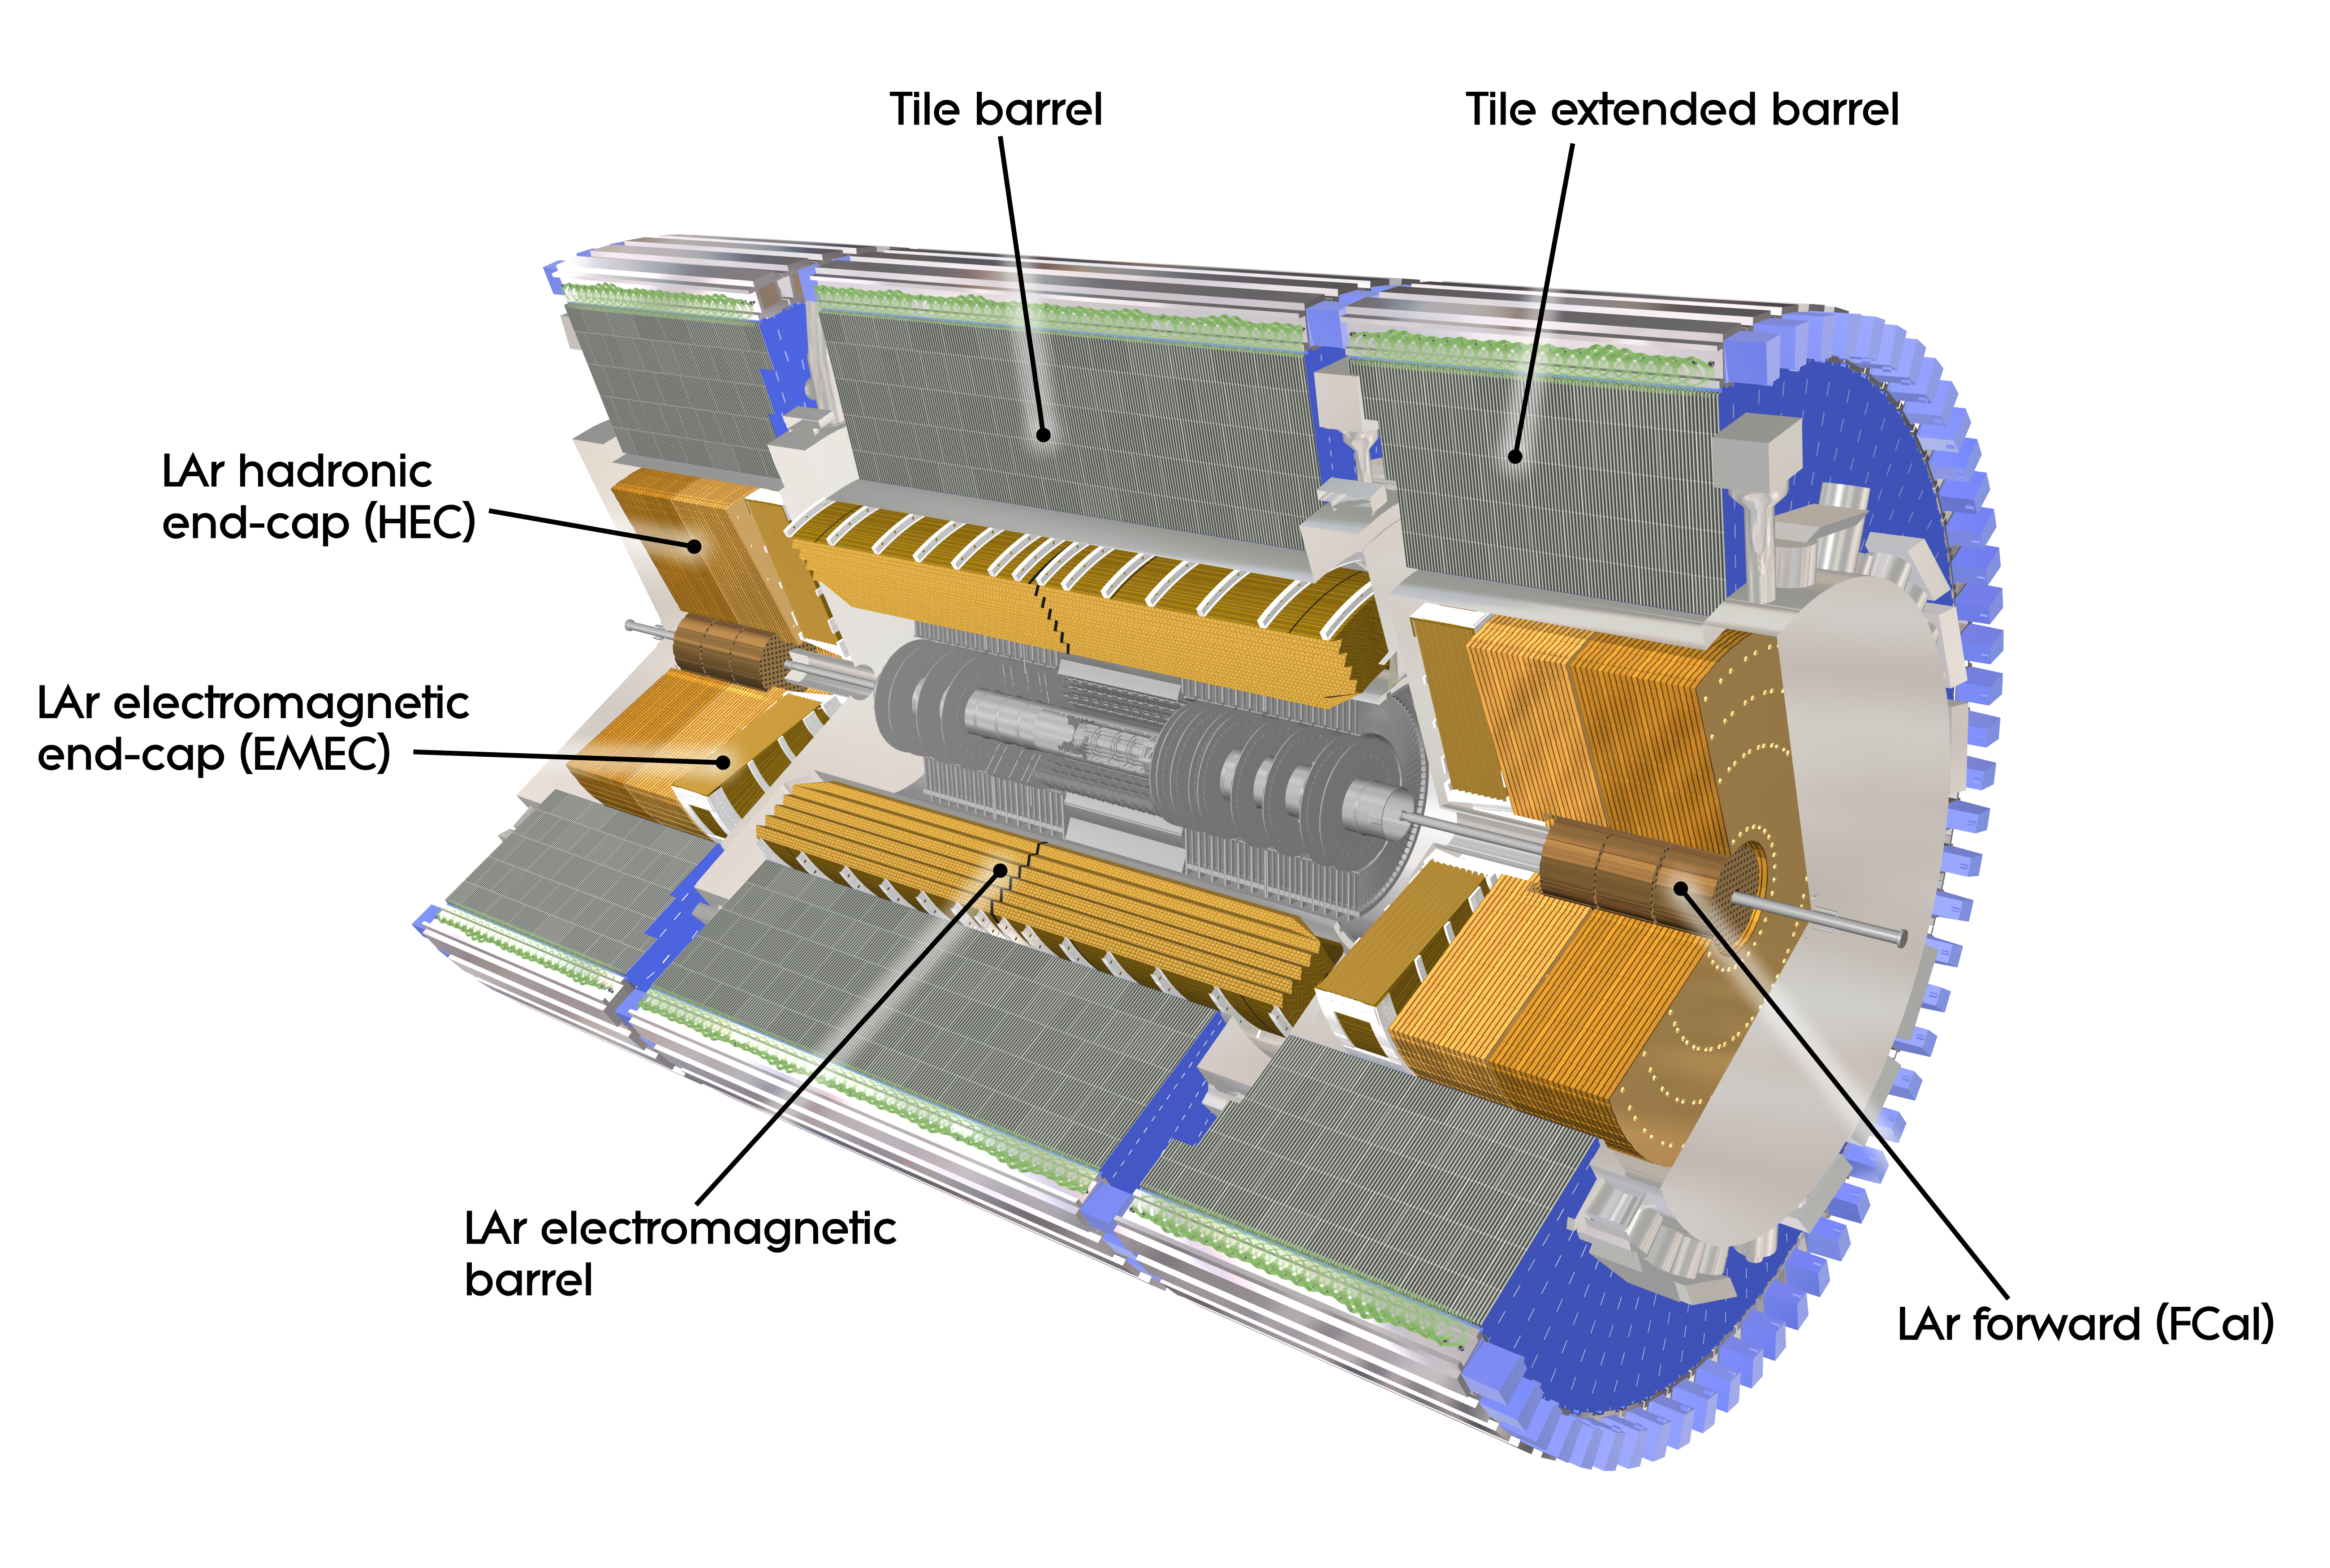
\includegraphics[width=\textwidth]{imagens/calorimetros.jpg}
\caption{Os diversos calorimetros do ATLAS. Extraido de
\cite{muons_images}.}
\label{fig:espec_muons}
\end{figure}

\subsection{O Espectômetro de Mûons}
\label{ssec:espectometro_muons}

\newacronym[type=Abrev]{mdt}{MDT}{Câmaras de Tubos de Movimento Monitorados}
\newacronym[type=Abrev]{csc}{CSC}{Câmaras de Tiras Catódicas}
\newacronym[type=Abrev]{rpc}{RPC}{Câmaras de Chapas Resistivas}
\newacronym[type=Abrev]{tgc}{TGC}{Câmaras de Brechas Finas}

\begin{figure}[h!t]
\centering
\includegraphics[width=0.8\textwidth]{imagens/espectometro_muons_lowres.jpg}
\caption{O Espectômetro de Mûons e seus componentes. Extraido de
\cite{muons_images}.}
\label{fig:espec_muons}
\end{figure}

Os mûons como estados finais são muito importantes em diversas análises e provêm
assinaturas físicas robustas no \gls{lhc}. 
Eles penetram grandes quantidades de material quando a maior parte das outras
partículas são absorvidas, e com o objetivo de medir sua energia, o Espectômetro
de Mûons \cite{muon_tdr} é o subdetector mais externo do \gls{atlas}. Diferente dos calorimetros
que emprega um processo de medição destrutivo, o Espectômetro de Mûons,
Figura~\ref{fig:espec_muons}, mede a carga e o momento de mûons através 
da reconstrução de suas trajetórias no 
campo magnético dos toróides de núcleo a ar de forma semelhante ao \gls{id}. 

As câmaras no barril formam três cilindros
concêntricos com o eixo dos feixes e cobrem um alcance em $|\gls{eta}| < 1$,
estando localizadas a uma distância radial de $\sim$5, 7,5, e 10m. São
utilizados quatro discos para as câmaras da tampa que cobrem um o alcance de 
$1 < |\gls{eta}| < 2,7$ em distâncias de $\sim$7, 10, 14 e 21-23 m do ponto de
interação, todos concêntricos ao tubo do feixe. Deseja-se medir mûons
na região de poucos GeV com uma resolução de $\sim1\%$, enquanto mûons na
faixa de 1 TeV a precisão pode ser um pouco menor, $ < 10\%$. O poder de
curvatura $Bl^2$ fornecido pelos toróides e tamanho do detector é de cerca de 36
$\text{Tm}^2$, comparado com os 2 $\text{Tm}^2$ no \gls{id}. Para fornecer a
resolução de momento desejada a \gls{respos} deve ser de no mínimo
50 $\mu$m em z e 0,5 mrad em R$\phi$ \cite{ATLAS_TDR}.

Existem diversos tipos de câmaras de traços de mûons: As \gls{mdt} e \gls{csc}
são as câmaras de precisão, já as \gls{rpc} e \gls{tgc} são câmaras
rápidas para o \glslink{l1}{Primeiro Nível de filtragem (L1)}. O príncipio de leitura é o mesmo para os quatro
tipos, onde os mûons que passam por uma fenda de gás entre um anôdo e catodo (por
exemplo, um cabo dentro de um tubo ou duas chapas paralelas) causam uma discarga
local no gás sendo assim possível ler o sinal. No total existem 5376 câmaras
com 1,0757 M canais de leitura \cite{tese_jatos}.

Os \glspl{mdt} fornecem medições de precião (acurácia mecânica de 30 $\mu$m) 
dos pontos do traço com 80 $\mu$m de \gls{respos}
para cada cabo em uma larga região de \gls{eta}. Em grandes \gls{eta} e próximo
do ponto de interação são utilizados os \glspl{csc}, que têm uma maior
granularidade e suportam a sua alta demanda causada pelas condições de ruído
físico.
 
As câmaras de filtragem tem uma resolução de tempo menor que o espaçamento
mínimo entre pacotes de 25 ns para fazer possível sua identificação. Os
requerimentos de tempo e espaço são atendidos de acordo com a seguinte
especificação: os \glspl{rpc} têm boa resolução de tempo (1,5 ns), por outro
lado os \glspl{tgc} tem melhor resolução espacial 
(o afastamento entre os cabos anôdos é de 1,8 mm).

Graças a grande dimensão do Espectômetro de Mûon não é possível de firmar as
dimensões e posições das câmaras no nível requerido de 30 $\mu$m. Portanto, as
deformações e posições da câmara são constantemente monitoradas por meio de
sistemas opticos de alinhamento, de forma que deslocamentos dentre $\approx$ 30
$\mu$m e $\approx$ 1 cm podem ser corrigidos em análise pelos algoritmos do
Sistema de Reconstrução \cite{muon_tdr}.

\section{Ferramentas Utilizadas na Colaboração}
\label{sec:ferramentas}


\chapter[Reconstrução da Física do Canal eGamma do Experimento ATLAS]
{Reconstrução da Física do Canal e/$\gamma$ do Experimento ATLAS}
\label{cap:reco}

\newacronym[type=Abrev]{t2calo}{\emph{T2Calo}}{Algoritmo para a Reconstrução do
Calorímetro no Segundo Nível de Filtragem} 
\newacronym[type=Abrev]{hltringer}{\emph{HLT\_Ringer}}{HLT\_EgammaCaloRinger} 
\glsunset{t2calo}

A alta energia e luminosidade do \gls{lhc} (Seção~\ref{sec:lhc}) oferecem um alto alcance para
explorar física, desde a medição precisa de propriedades de objetos conhecidos, a
ultrapassar a fronteira de energias onde a física ainda não havia sido experimentada.
Por ser um detector de propósito geral, o \gls{atlas} (Seção~\ref{sec:ATLAS}), deve ser capaz de
explorar diversos dos objetivos do \gls{lhc} (Subseção~\ref{ssec:obj_lhc}), e
para isso ele precisar ter a capacidade de explorar um largo espectro de assinaturas
físicas. Esse fato guiou a otimização do projeto do \gls{atlas}, dando as especificações de sensibilidade e precisão do
detector para que seja possível através das assinaturas realizar a reconstrução
com precisão da física ocorrida nas colisões. O foco principal é na busca pelo
bóssom de Higgs \cite{ATLAS_TDR2}, com o objetivo de provar a origem da escala
eletrofraca\footnote{A escala eletrofraca existe somente no estado primitivo descrito na
Subseção~\ref{ssec:bossoms}.}. 

A física se apoia em algoritmos
para realizar a busca pelas assinaturas, sendo este capítulo dedicado aos
algoritmos que fazem a reconstrução do Canal \gls{eg},
onde se deseja encontrar as assinaturas dessas partículas (e dos pósitrons, que
tem a mesma assinatura de elétrons, excluindo a direção de deflexão de seus
traços, oposta àquela de elétrons devido a sua carga positiva). A identificação
dessas partículas é de fundamental importância por formarem os canais de
decaimentos mais limpos do bóssom de Higgs (Sessão~\ref{sec:busca_higgs}). Além
disso, outras partículas como o bóssom Z e partícula $\text{J}/\Psi$, podem ser
utilizadas para melhorar a escala de medida de energia dos calorímetros e
estudar sua linearidade de resposta por terem suas massas bem conhecidas, 
em especial os decaimentos de elétrons do
$\text{J}/\Psi$ para baixas energias ($\gls{Et} > 5$ GeV), onde se esperam encontrar 
decaimentos leptônicos do bóssom de Higgs de menor energia ($\gls{Et} > 7$ GeV).
Outras assinaturas experimentais são as de hádrons e jatos, que serão tratadas
quando abordando o Canal \gls{eg}, por serem o ruído de fundo do qual se deseja
filtrar nesse canal. Entretanto existem setores de física que se
interessam por esses decaimentos, como o já citado decaimento do bóssom W em jatos
duplos\footnote{A citação foi realizada no Subtópico~\ref{par:cal_part_id}.}. 
Além disso, múons constituem de outras assinaturas, uma vez que interagem
pouco com os calorímetros, tendo seu próprio subsistema, o Espectômetro de
Múons. Existem outras três assinaturas:
táons, sabores pesados e léptons neutrinos. Os táons decaem
rapidamente em múons (ou elétrons) e mais dois neutrinos, ou ainda, em um ou três
píons carregados, de forma que sua assinatura é
feita nos espectometros de múons (ou calorímetro), ou de chuveiros \gls{had} com um ou três
traços isolados apontando para o chuveiro. Os sabores pesados procuram
assinaturas de mésons pesados, que geralmente decaem a menos de 1 mm do ponto de
colisão, sendo necessário criar um vértice secundário que será identificado com
a alta precisão do Detector de Pixel. Finalmente, léptons neutrinos escapam da
deteção, para sua assinatura é utilizada a propriedade de conservação de
\gls{pt}, de modo que, quando há quantidade suficiente de \gls{ptmiss}, há indicios
de que algo escapou do processo de deteção.

Os algoritmos são implementados em dois ambientes diferentes, um ambiente mais
restrito, necessário devido ao alto nível de ruído físico gerado nas condições 
impostas do \gls{lhc} (citadas no Tópico~\ref{sssec:minb_ue_pileup}): o
\glsdesc{sf} (Seção~\ref{sec:sf}). Nesse ambiente o tempo de discriminação 
é limitado a latência suportada pela capacidade computacional das máquinas localizadas 
no \gls{ip}1. O trabalho segue com o desenvolvimento do algoritmo
\acrlong{hltringer} (Subseção~\ref{ssec:hlt_ringer}), um algoritmo alternativo proposto para o
Segundo Nível de Filtragem desse sistema. A versão implementada pela
colaboração, o \gls{t2calo} (Subseção~\ref{ssec:cadeia_egamma}), 
também é descrita em detalhes. Por sua vez o outro ambiente, o \glsdesc{sr}
(Seção~\ref{sec:sr}), visa fazer uma análise mais precisa dos eventos de colisão e da 
física gerada, sendo o \glsdesc{sf}, nos níveis mais altos de filtragem, 
nada mais que uma versão restringida baseada no mesmo. Para que a Colaboração tenha 
um melhor contato com o algoritmo proposto e entenda o seu funcionamento, se fez
necessário a implementação (Tópico~\ref{sssec:egringer_impl}) de uma versão no Sistema 
de \glsdesc{sr} (Subseção~\ref{ssec:egringer}) para que os físicos o utilizassem nas suas 
análises a posteriori. A versão padrão (Subseção~\ref{ssec:egamma}) utilizada
pelos físicos também foi abordada.


\section{Busca pelo bóssom de Higgs}
\label{sec:busca_higgs}

\newacronym[type=Simb]{mh}{\ensuremath{m_H}}{massa do bóssom de Higgs} 
\newacronym[type=Abrev]{lep}{LEP}{\emph{Large Electron Positron Collider}} 
\glsunset{mh}

O bóssom de Higgs no setor do \gls{mp} é amplamente irrestrito, de forma que sua
massa, \acrshort{mh}, não é prevista pela teoria. Um limite superior na ordem de
$\sim$1 TeV teórico, e um limite inferior experimental\footnote{As exclusões
citadas foram feitas para um nível de confiança de 95\%.\label{fn:95cl}} de 95,2
GeV \cite{lep_higgs_1999} por um experimento anterior do \gls{cern}, o \gls{lep}, determinam a região para a qual
se esperava encontrar o bóssom de Higgs durante a época das últimas propostas técnicas
do projeto do \gls{atlas} \cite{ATLAS_TDR,ATLAS_TDR2}, por volta de 1999. 

Um estudo do potêncial de descoberta do bóssom de Higgs através de seus
possíveis canais de decaimentos explorados pelo programa de física do
\gls{atlas} foi revisado na propostas citadas. Esses canais são:

\begin{itemize}
\item $H\rightarrow\gamma\gamma$ (110 a 150 GeV/$c^2$), produção direta;
\item $H\rightarrow\gamma\gamma$ (110 a 150 GeV/$c^2$), da produção associada $WH$, $ZH$ e
$t\bar{t}H$, usando um lépton (e, $\mu$) rotulado do decaimento dos bóssom W, Z ou
do quark \emph{top};
\item $H\rightarrow b\bar{b}$ (110 a 130 GeV/$c^2$), da produção associada $WH$, $ZH$ e
$t\bar{t}H$, usando um lépton (e, $\mu$) rotulado do decaimento dos bóssom W, Z ou
do quark \emph{top};
\item $H\rightarrow ZZ^*\rightarrow4l$ (110 a 600 GeV/$c^2$. O símbolo $^*$ representa uma partícula 
que está fora de sua fronteira de massa\footnote {Na literatura em inglês 
\emph{off the mass shell}, ou simplesmente \emph{off
shell}.} na relação massa-momento dada pela equação~\ref{eq:rel_mom}. Essas
partículas só existem como estados intermediários, constituindo partículas
virtuais, e estão de acordo com o princípio da incerteza, em que as partículas
só podem existir nesse estado durante um tempo menor que uma fração da
constante 
de Plank pela diferença de energia, ou $\Delta E \Delta t \gtrsim h$), onde l
representa estes léptons: $e,\mu$; 
\item $H\rightarrow ZZ\rightarrow4l$ e $H\rightarrow ZZ\rightarrow ll\nu\nu$i
(200 a 600 GeV/$c^2$), aqui $\nu$ são os léptons neutrinos;
\item $H\rightarrow WW\rightarrow l\nu jj$ e $H\rightarrow ZZ\rightarrow ll jj$
($\sim$600 a 1 TeV),
onde $jj$ representa o decaimento em jatos duplos;
\item $H\rightarrow WW^*\rightarrow l\nu l\nu$ (110 a 300 GeV/$c^2$). 
\end{itemize}


Nesse estudo se utilizou simulações
de Monte Carlo do \emph{Pythia}, através da significância desses 
canais numa região de 80-1000 GeV/$c^2$ (lembrando que na época só havia sido excluído
o bóssom de Higgs para \gls{mh} < 95,2), utilizando os valores de resposta dos
subdectores, resolução e capacidade esperadas de identificação de sinais e rejeição 
de ruídos redutivéis. 
Os resultados desse estudo estão resumidos na Figura~\ref{fig:higgs_sim_atlas},
mostrando a significância do sinal para uma luminosidade integrada\footnote{A 
luminosidade integrada, como seu nome indica, não passa da integral da luminosidade 
instantânea no tempo de operação do \gls{lhc}: $\int{L_{inst} dt}$.} de
100 $\text{fb}^{-1}$. Para efeito de comparação na
Figura~\ref{fig:higgs_branch_ratio} há as relações entre os canais
e seus alcânces em massa. A Figura~\ref{fig:higgs_production} contêm a seção
de choque esperada para as possíveis massas.

\begin{figure}[ht!]
    \label{fig:higgs_expected}
    \begin{center}
%
        \subfigure[]{%
            \label{fig:higgs_branch_ratio}
            \includegraphics[width=0.47\textwidth,height=6cm]{imagens/higgs_branch_ratio.pdf}
        }%\hspace{0.1\textwidth}
        \subfigure[]{
            \label{fig:higgs_production}
            \includegraphics[width=0.47\textwidth,height=6cm]{imagens/higgs_production.pdf}
        }\\
        \subfigure[]{%
            \label{fig:higgs_sim_atlas}
            \includegraphics[width=.6\textwidth]{imagens/higgs_sim_atlas.pdf}
        }
    \end{center}
\caption[Simulação da significância dos canais de decaimento do bóssom
de Higgs explorados pelos ATLAS, as relações de seus canais e alcances em massa,
e a seção de choque do mesmo.]
{Os decaimentos do bóssom de Higgs do MP e suas relações de
seus canais e alcances em massa,~\ref{fig:higgs_branch_ratio}, e os seus valores de seção de choque para suas
repectivas massas,~\ref{fig:higgs_production}, ambos extraídas de \cite{lhc_higgs_group}. 
Em \ref{fig:higgs_sim_atlas} está uma simulação da significancia dos possíveis canais de decaimento do
bóssom de Higgs, explorados pelo ATLAS, para uma luminosidade integrada de
$100fb^{-1}$, utilizando as eficiências esperadas para a deteção das
assinaturas dos estados finais e resoluções dos subdetectores, extraído de
\cite{ATLAS_TDR2}.}
\end{figure}

Observe que decaimentos do bóssom de Higgs mais frequentes não são,
necessariamente, os canais com melhor significância esperada. Aqueles canais em
que se tem mais facilidade de observar os decaimentos finais e poder associá-los
a produção de um bóssom de Higgs podem ter mais significância do que canais com
maior produção para uma dada massa. Isso reflete, por outro lado, na importância
dos algoritmos de reconstrução, obtendo melhor eficiência na reconstrução dos
estados finais facilitariam a encontrar o bóssom com menor quantidade de dados.
Os canais mais importantes nas regiões de massa intermediária, $\gls{mh}<2m_Z$,
onde se espera que os decaimentos reconstruam um pico de massa, são 
o canal de quatro léptons, $H\rightarrow ZZ^* \rightarrow 4l$, o canal de
produção direta em dois fótons, $H\rightarrow \gamma\gamma$, junto com os
canais de produção associada com o mesmo estados finais, . Para massas por volta
de 170 GeV/$c^2$, onde a produção de $ZZ^*$ é suprimida, o potêncial da descoberta do
Higgs pode ser elevada pelo decaimento $H\rightarrow WW^*\rightarrow l\nu l\nu$,
nesse caso, o sinal deverá ser observado como um excesso de eventos. O canal de
quatro léptons com dois bóssoms Z reais é o dominante na região de
$\gls{mh}>2m_Z$, cobrindo uma vasta região de massa\footnote{Por isso chegou a
ser referênciado como canal banhado a ouro.}. Em massas mais elevadas, por volta de 600 GeV/$c^2$ até 1
TeV, outros canais como $H\rightarrow WW\rightarrow l\nu jj$, $H\rightarrow
WW\rightarrow ll\nu\nu$ são utilizados para a busca do bóssom de Higgs.

Posteriormente, outro canal foi adicionado, por outros estudos
\cite{atlas_tautau,atlas_tautau2}:

\begin{itemize} 
\item $H\rightarrow \tau \tau \rightarrow ll4\nu$ e $H\rightarrow \tau \tau
\rightarrow l\tau_{had}3\nu$ (110 a 150 GeV/$c^2$), onde $\tau_{had}$ seria o
decaimento do táon em píons especificados no início deste capítulo.
\end{itemize} 

Assim, a reconstrução de elétrons e múons fazem parte de grande
parte dos canais explorados para a vasta região de massa em que se espera
encontrar o bóssom de Higgs, inclusive um dos canais
mais importante por cobrir uma vasta região de massa. Se o Higgs existir com
uma massa mais baixa, os fótons serão necessários para poder encontrar o bóssom,
mostrando a importância do Canal \gls{eg}. 

\begin{figure}[t!]
    \label{fig:higgs_exclusion}
    \begin{center}
    \includegraphics[width=0.8\textwidth]{imagens/exclusion_cms_atlas.pdf}
%
%        \subfigure[LEP, extraído de \cite{lep_higgs_2008}.]{%
%            \label{fig:lep_exclusion}
%            \includegraphics[width=0.47\textwidth]{imagens/lep_exclusion.pdf}
%        }%\hspace{0.1\textwidth}
%        \subfigure[Tevatron, extraído de \cite{tevatron_higgs}.]{%
%            \label{fig:tevatron_exclusion}
%            \includegraphics[width=0.47\textwidth]{imagens/tevatron_exclusion.pdf}
%        }\\%\hspace{0.1\textwidth}
%        \subfigure[ATLAS, extraído de \cite{atlas_higgs}.]{
%            \label{fig:atlas_exclusion}
%            \includegraphics[width=0.47\textwidth]{imagens/atlas_exclusion.pdf}
%        }
%        \subfigure[CMS, extraído de \cite{cms_higgs}.]{%
%            \label{fig:cms_exclusion}
%            \includegraphics[width=0.47\textwidth]{imagens/cms_exclusion.pdf}
%        }
    \end{center}
\caption[Exclusões de massa do Higgs realizada pela combinação dos dados do
ATLAS e CMS. As exclusões de massa do Tevatron e LEP também estão indicadas.]{As exclusões de massa do bóssom de Higgs. Os valores de massa
observados, no caso para os resultados combinados do ATLAS e CMS, quando
abaixo da linha horizonal vermelha indicada são excluídos com um nível de
confiança de 95\%. A linha pontilhada indica o ruído de fundo esperado gerado
por física na ausência do bóssom de Higgs. As faixas verdes e amarelas indicam
um nível de certeza de 68\% e 95\% de certeza de que algo fora do comum está
ocorrendo. Caso a linha observada ultrapasse o limite superior da faixa amarela
em regiões acima da linha vermelha, então há 95\% de certeza de que há indicios
do bóssom de Higgs ou algum processo de física (talvez ruído físico) não bem
conhecido. Extraído de \cite{atlas_cms_higgs}.}
\end{figure}

Resultados mais recentes excluiram outras regiões de massa do bóssom de Higgs. Em 2008, 
o legado deixado pelo \gls{lep} elevou o limite inferior para 114 GeV/$c^2$
\cite{lep_higgs_2008}, enquanto o experimento Tevatron realizado pelo Fermilab, excluiu as
regiões de $156 < \gls{mh} < 177$ GeV/$c^2$, em Setembro de 2011
\cite{tevatron_higgs}. Também no final de Setembro, resultados preliminares do
\gls{atlas} excluiram o bóssom de Higgs para as regiões de 146-230 GeV/$c^2$, 256-282 GeV/$c^2$ 
e 296-459 GeV/$c^2$ \cite{atlas_higgs}. Um mês antes o \gls{cms} havia excluido o bóssom para
as regiões parecidas: de 145-216 GeV/$c^2$, 226-288 GeV/$c^2$ e 310-400 GeV/$c^2$
\cite{cms_higgs}. Em meados de Novembro o \gls{atlas} e \gls{cms} uniram seus
dados para excluir a região de 141-476 GeV/$c^2$ \cite{atlas_cms_higgs}. Esses
resultados estão indicados na Figura~\ref{fig:higgs_exclusion}, onde estão os
resultados mais recentes do \gls{lhc}, incluidas das regiões anteriormente
excluídas por outros experimentos.


\section{O Sistema de Filtragem (SF)}
\label{sec:sf}

\newacronym[type=Abrev]{asic}{ASIC}{Circuitos Integrados de Aplicação Específica}

O \gls{atlas}, para a luminosidade na qual tem operado: $\sim10^{33}cm^{-2}s^{-1}$,
gera cerca de 19 colisões inelásticas para cada cruzamento entre
feixes, que irão se cruzar numa frequência máxima de 40 MHz. O propósito do
\gls{sf} \cite{trigger_perf_2010,trigger_tdr} é de reduzir essa taxa a cerca
de 200 Hz para seu armazenamento e processamento a posteriori. Esse
limite, correspondendo uma média de $\sim$300 MB/s, é determinado pelos recursos
computacionais para armazenamento e processamento dos dados. É possível gravar
dados com taxas relativamentes mais altas por períodos mais curtos, como foi
realizado durante 2010 quando a física foi beneficiada utilizando taxas de saída
de até $\sim$600 Hz. Nessa época, a luminosidade instantânea máxima atingida foi de
$\sim10^{32}cm^{-2}s^{-1}$, gerando cerca de $\sim$ 1,3 MB, e o \gls{lhc} não 
operava de forma continua -- o que é comum para um acelerador novo -- permitindo 
elevar a taxa de armazenamento.

\subsection{A estrutura do Sistema de Filtragem}
\label{ssec:estru_sf}
\newacronym[type=Abrev]{rob}{ROB}{\emph{Buffer} de Leitura}
\newacronym[type=Abrev]{ros}{ROS}{Sistemas de Leitura}

O \gls{sf}, Figura~\ref{fig:sf_esboco}, é dividido em três níveis sequenciais,
sendo descrito aqui resumidamente uma vez que já foi explicada em maiores detalhes em
trabalhos anteriores como \cite{tese_eduardo,tese_torres}, também podendo ser encontrada 
em detalhes nas referências \cite{trigger_tdr,l1_trigger_tdr,l2_ef_daq_dcs_tdr,trigger_perfomance}.

Os sinais do detector são armazenados em memórias \emph{pipeline}, com pendência
à decisão do \acrshort{l1}. Para obter uma latência de menos de 2,5 $\mu$s, 
o \gls{l1} é implementado em rápida eletrônica constituída de \gls{fpga} e
\gls{asic}, de forma a reduzir a taxa para uma valor máximo de 75 kHz. Para
aumentar a velocidade, esse nível utiliza apenas a informação dos subsistemas de
calorimetria e câmaras de mûons com granularidade reduzida. Além do
primeiro passo de seleção, o \gls{l1} identifica as \glspl{roi} do detector a
serem investigadas pelo \acrshort{hlt}. 

\begin{figure}[ht!]
\label{fig:sf_esboco}
\centering
\includegraphics[width=0.6\textwidth]{imagens/sf_resumo.pdf}
\caption[Esboço do Sistema de Filtragem.]{Esboço do Sistema de Filtragem. Extraído de \cite{tese_eduardo}.}
\end{figure}

O \gls{hlt} se consiste de fazendas de
processadores comerciais conectados a rede dedicadas (\emph{Ethernet} de \emph{Gigabit} 
e 10 \emph{Gigabit}).  O \gls{sf} foi projetado para conter cerca de 500 nós para o
\acrshort{l2} e 1800 nós para o \acrshort{ef}\footnote{Em 2010, a fazenda de processamento 
se consistia de 800 nós configuraveis como tanto \acrshort{l2} ou \acrshort{ef}, este 
contendo mais 300 nós dedicados.}. Quando um evento é aceito pelo
\gls{l1}, os dados na memória de cada um dos detectores são então transferidos
para \gls{rob} específicos para cada um dos subdetectores, que armazenam o
evento em fragmentos pendendo à decisão do \gls{l2}. Um ou mais \glspl{rob} são
agrupados para formar os \gls{ros} que são conectados a rede do \gls{hlt}. O
seleção do \gls{l2} é baseada em algoritmos personalizados e rápidos que
processam os dados dos eventos de forma parcial nas regiões especificadas pelas
\glspl{roi} identificadas pelo \gls{l1}. Os processores do \gls{l2} solicitam os
dados dos \gls{ros} correspondentes aelementos do subdetector dentro de cada
\gls{roi}, reduzindo a quantidade de dados a serem transferidas e processadas no
mesmo a cerca de 2-6\% do volume total dos dados. O \gls{l2} reduz a taxa de
dados para cerca de $\sim$3 kHz com uma média de processamento de $\sim$40
ms/evento. Qualquer evento com tempo excedendo a 5 s nesse nível é perdido a
rotulado como evento excedente ao tempo limite.   

O \gls{ef} reune todos os framentos dos eventos aceitos pelo \gls{l2} das
\glspl{rob}, tendo assim acesso a toda sua informação. O \gls{ef} é, em grande
maioria, baseado nos algoritmos do \acrlong{sr} rodando em interfaces
personalizadas para o ambiente do \gls{sf}. Esse nível é projetado para reduzir
os dados para $\sim$200 Hz com uma média de processamento de $\sim$4 s/evento.
Qualquer evento com um tempo excedente a 180 s também é rotulado e perdido como
no \gls{l2}. 

Os eventos de dados selecionados pelo \gls{sf} são escritos nos fluxos de dados
inclusivos, baseados no canal de filtragem. Existem quatro canais de dados
primários: Egamma, Muons, JetTauEtMiss, Minbias, adicionados de diversos canais
de calibração. Cerca de 10\% dos eventos são escritos para um canal expresso
aonde a reconstrução pronta dos eventos é realizada, como foi dito na
Subseção~\ref{ssec:lcg}. Ainda, além da gravação de evnetos completos em um
canal, é possível escrever informação parcial de um ou mais subdetectores em um
canal, o que é normalmente realizado para a calibração do detector nos canais
destinados a esse propósito.

\subsection{Topologia dos algoritmos e sua configuração}
\label{ssec:alg_topo}

\newacronym[type=Abrev,\glslongpluralkey={Algoritmos de Extração de
Características}]{fex}{FEX}{Algoritmo de Extração de Característica}
\newacronym[type=Abrev,\glslongpluralkey={Algoritmos de Hipótese}]
{hypo}{HYPO}{Algoritmo de Hipótese}

A configuração do \gls{sf} é realizada por um \emph{menu}, que define as
\emph{cadeias} de filtragem que especificam uma sequência de passos de reconstrução e
seleção para as especificas assinaturas de filtragems requeridas pela filtragem.
A cadeia de filtragem de elétrons é ilustrada na Figura~\ref{fig:electron_chain}.
Cada \emph{cadeia} é composta por \gls{fex} que criam objetos,
como os aglomerados de células e variáveis que permitam obter uma informação
sobre a descrição do evento, e \gls{hypo} que fazem a discriminação através dos
critérios de seleção nos objetos gerados, como por exemplo a exigência de um
$\gls{pt} > 20$ GeV. As extrações de características realizadas por uma
\emph{cadeia} podem ser reutilizadas por outro cadeia, reduzindo tanto o acesso
a dados como o tempo de processamento do \gls{sf}.

\begin{figure}[ht!]
\label{fig:electron_chain}
\centering
\includegraphics[width=0.9\textwidth]{imagens/cadeia_eletron.png}
\caption[A \emph{cadeia} de filtragem de elétrons.]{A \emph{cadeia} de filtragem
de elétrons. A direita de cada nível de filtragem estão colocados exemplos de
nomes de filtros de elétrons e fótons, e o nome de sua respectiva cadeia a
direita da seta indicando a evolução da \emph{cadeia}. Adaptado de \cite{trigger_perf_2010}.}
\end{figure}

Aproximadamente 500 filtros são definidos nos \emph{menus} atuais, sendo
composto por um número de diferentes classes de filtros:

\begin{enumerate}
\item \textbf{Objetos de filtro único}: usado para determinar estados com pelo
menos um objeto característico. Por exemplo, um filtro para elétron único com um
limiar nominal superior a 3 GeV seria referido como $e3$;
\item \textbf{Objetos de filtro multiplos}: usado para determinar estados finais
com dois ou mais objetos do mesmo tipo. Por exemplo, elétrons duplos decaindo da
partícula $\text{J}/\Psi$. Esses filtros são indicados dependendo de sua
multiplicidade, por exemplo: $2e3$;
\item \textbf{Objetos de filtro combinados}: usados por estados finais de dois
ou mais objetos característicos de tipos diferentes. Por exemplo, um múon de 13
GeV adicionado de 20 GeV de \gls{Etmiss} para selecionar decaimentos
$W\rightarrow \mu\nu$, que seriam denotados de $mu13\_xe20$;
\item \textbf{Filtros Topológicos}: usados para estados finais selecionados de
duas ou mais \glspl{roi}, como no caso do decaimento da partícula
$\text{J}/\Psi$, que combina os traços das duas \glspl{roi} provenientes dos
elétrons.
\end{enumerate}

Quando se referindo a um nível em partícular, o nível (\gls{l1}, \gls{l2},
\gls{ef}) aparece como um prefixo, como por exemplo L1\_EM3 (aqui elétrons e
fótons não são diferenciados, então se utiliza o prefixo EM em ambos os casos)
para denotar um filtro de elétrons e fótons com um limiar nominal superior a 3
GeV para o \gls{l1} e L2\_e3 no caso de elétrons para um filtro com o mesmo
limiar mas para elétrons apenas no \gls{l2}. Um nome sem o prefixo de nível
refere-se a toda a \emph{cadeia}.

O controle das taxas de filtragem podem ser realizadas mudando os limiares ou
aplicando outros valores de seleção. A seletividade de um grupo de cortes
aplicados para um certo objeto de filtragem é representado pelos termos
\emph{Loose} (frouxo), \emph{Medium} (mediano), \emph{Tight} (apertado). Esses
critérios de seleção são colocados como sufixos ao nome do filtro, por exemplo,
e10\_medium. Requerimentos adicionais como isolamento, podem ser adicionados
para reduzir as taxas dos filtros. O isolamento mede a quantidade de energia, ou
o número de partículas próximos a uma assinatura, se esse valor estiver acima de
um limiar, então a partícula não está isolada. Nesse caso se adiciona a letra
'i' ao nome do filtro, como por exemplo L1\_EM20I ou e20i\_tight.

Fatores de \emph{pré-escala} podem ser adicionados a cada filtro da 
\emph{cadeia} do \gls{hlt}, de tal forma que apenas 1 em cada N eventos passando
o filtro causam que o evento seja aceito por aquele nível. A \emph{pré-escala}
controla a taxa e composição dos canais expressos. Uma série de
\emph{pré-escalas} são utilizadas baseadas em diversas regras que levam em
consideração a prioridade dos filtros em relação com as seguintes categorias:

\begin{enumerate}
\item \textbf{Filtros Primários}: filtros princípais de física, que não deveriam
ser \emph{pré-escalados};
\item \textbf{Filtros de Suporte}: filtros importantes de suporte a filtros
primários, como filtros que permitam estudar a eficiência utilizando 
seletividades mais baixas e limiar mais baixo de \gls{Et} \emph{pré-escalados}
para permitir sua gravação em disco, uma vez que a quantidade de dados que
passam esse filtro será maior;
\item \textbf{Filtros de Monitoração e Calibração}: permitindo a coleta de dados
para garantir a operação correta do \gls{sf} e dos subdetetores do \gls{atlas},
incluindo a calibração dos mesmos. 
\end{enumerate}

\newacronym[type=Abrev]{lb}{LB}{Bloco de Luminosidade} 

Esses fatores de \emph{pré-escala} devem ser modificados conforme a queda da
luminosidade durante um preenchimento do \gls{lhc} de forma a garantir a
maximização das taxas utilizadas pelos filtros, enquanto garantindo uma taxa
constante para a monitoração e calibração. Assim, as mesmas podem ser alteradas
em quaisquer momentos de uma temporada, no início de um novo \gls{lb}. Um
\gls{lb} é a unidade fundamental para a medição da luminosidade, cerca de 120 s
em 2010, na qual se considera que a mesma permaneceu constante com o valor
medido.

Flexibilidade adicional é oferecida ao definir \emph{grupos de pacotes}, separando os
filtros para colisões com pacotes emparelhados (compõe as colisões de física
regulares, contendo pacotes de feixes opostos que se encontram no ponto de
colisão simultaneamente), pacotes vazios para estudo de pedestal criado por ruído 
no detector e raios cósmicos, ou até mesmo configurações mais inusitadas, como 
exigindo pacotes desparelhados separados por no mínimo 75 ns de quaisquer outro 
pacote no feixe oposto.

\subsection{Algoritmos Padrões da \emph{Cadeia} de Filtragem de Elétrons e Fótons}
\label{ssec:cadeia_egamma}

\newacronym[type=Abrev,\glslongpluralkey={Torres de Filtragem}]
{tt}{TT}{Torre de Filtragem}

O sistema de calorimetria do \gls{atlas} cobre uma região de $|\gls{eta}| <
4,9$, enquanto o \gls{id} fornece reconstrução precisa de traços dentro de
$|\gls{eta}| < 2,5$. Os chuveiros \gls{em} são reconstruídos com melhor
performance para essa última região, a região de precisão do \gls{atlas}, 
contendo calorímetros com maior granularidade como descrito na
Subseção~\ref{ssec:calorimetria}. Assim, os filtros de elétrons e fótons
\cite{expected_perf_2011,perf_2011} do \gls{sf} atuam somente para essa região.
A cadeia de elétrons no \gls{sf} está esboçada na Figura~\ref{fig:electron_chain}, entretanto
a cadeia de fótons pode ser facilmente extrapolada ao se remover os algoritmos
referentes ao \gls{id}.

No \gls{l1}, os aglomerados de informação\footnote{No caso, um conjunto de
células identificados como \emph{clusters} na literatura em inglês.} \gls{eg} do calorímetro são retirados
utilizando granularidade reduzida, as chamadas \glspl{tt}, que cobrem uma região
de aproximadamente $\Delta\eta\times\Delta\phi\approx0,1\times0,1$, 
a Figura~\ref{fig:cal_lar_camadas} contem um esboço da \gls{tt} para o
barril do calorimetro \gls{em}. A vantagem de se utilizar \glspl{tt} se deve ao
fato de reduzir a quantidade de fluxo de informação, reduzindo o custo e
complexidade do sistema, e, ao mesmo tempo, conter o chuveiro \gls{em} inteiramente 
em cerca de uma ou duas dessas torres, podendo
assim identificar a região em que foi formado o chuveiro não prejudicando a sua
eficiência. Para cada \gls{tt}, as células do calorímetro \gls{em} e \gls{had} são somadas, com a
excessão da quarta camada da tampa do calorímetro \gls{had} e dos cintiladores.
Um algoritmo de janela deslizante formada por uma dimensão de $4\times4$
\gls{tt}, ilustrada na Figura~\ref{fig:sliding_window_l1}, 
busca pela região com a melhor deposição de energia do chuveiro por
todo o calorímetro com um passo de uma \gls{tt}.
O \gls{l1} seleciona o evento como um candidato a \gls{eg} 
quando os seguintes critérios forem satisfeitos:

\begin{figure}[ht!]
\label{fig:l1_alg}
\centering
        \subfigure[A janela deslizante, seu núcleo e as regiões de isolamento.]{
            \label{fig:sliding_window_l1}
            \includegraphics[width=0.6\textwidth]{imagens/sliding_window_l1.pdf}
        }\hspace{0.01\textwidth}
        \subfigure[Requerimento para o núcleo ser máximo local.]{%
            \label{fig:local_et}
            \includegraphics[width=0.3\textwidth]{imagens/roi_local_max.pdf}
        }
\caption[O Primeiro Nível de Filtragem para a Cadeia de Elétrons e Fótons.]
{O Primeiro Nível de Filtragem para a Cadeia de Elétrons e Fótons. Extraído de
\cite{l1_trigger_tdr}.}
\end{figure}

\begin{itemize}
\item A região deve ser um máximo local. Essa condição é importante para se
evitar multiplicidade de \glspl{roi} a serem analisadas pelo \gls{l2}.
Assim, a energia contida no núcleo deve ser
maior, ou ao menos igual, como na lógica da Figura~\ref{fig:local_et}, 
que em todos as outras regiões de $2\times2$ que podem ser formados na
janela;
\item O aglomerado formado pela dupla de torre mais energética na região
(indicados na Figura~\ref{fig:sliding_window_l1} como somas verticais ou horizontais) deve ultrapassar o limiar
\gls{em} exigido pelo filtro do \gls{l1}. A posição de \gls{eta} e \gls{phi} desse aglomerado é passado
para o \gls{l2}, junto com outros \emph{bits} indicando os critérios que foram
satisfeitos, que formarão a palavra informada para o \gls{l2} para a qual será
utilizada para a formação da \gls{roi};
\item Se isolamento for exigido: 
\begin{itemize}
\item A \gls{Et} total da região \gls{em} de
isolamento não deve ultrapassar o limiar de isolamento \gls{em};
\item A \gls{Et} total da região \gls{had} de isolamento não deve ultrapassar o
limiar de isolamento \gls{had}.
\end{itemize}
\end{itemize}


O \gls{l2}, alimentado pela posição dos
aglomerados de torres do \gls{l1}, realiza uma rápida reconstrução do
calorímetro, e no caso de elétrons, uma rápida reconstrução dos traços no \gls{id}. A
reconstrução do calorímetro trabalha de maneira semelhante aos algoritmos do
\gls{sr}, entretanto apenas a região da janela de $\Delta\eta\times\Delta\phi =
0,4 \times 0,4$, região chamada de \gls{roi}, em torno da posição alimenda pelo \gls{l1} 
é utilizada, o que reduz o tráfico de dados e aumenta a velocidade de processamento no \gls{l2}.
Algumas diferenças entre o algoritmo do \gls{l2} e o \gls{sr} se dão as
limitações no tempo de latência. O algoritmo de reconstrução do aglomerado de
células do calorímetro no \gls{l2} começa utilizando a célula mais energética da
segunda camada \gls{em} dentro da região central de $0,2 \times 0,2$, enquanto o
algoritmo de análise a posteriori utiliza uma janela deslizante para encontrar
sua semente.

No \gls{l2}, o tamanho do aglomerado é fixado para $3
\times 7$ células em $\gls{eta} \times \gls{phi}$ para o barril ($|\gls{eta}|<1,5$) e 
$5 \times 5$ na tampa ($1,5<|\gls{eta}|<2,5$). O
algoritmo a posteriori contêm tamanhos de aglomerados diferentes, usando
$3\times5$ e $3\times7$ para fótons não convertidos e convertidos,
respectivamente, em $|\gls{eta}|<1,5$, e $5\times5$ até $|\gls{eta}|<2,5$.

As energias das células podem ser corrigidas na análise a posteriori, para
problemas transientes no \emph{hardware}, como falhas de energia, etc., o que não
pode ser realizado em tempo real, o que se aplica para tanto o \gls{l2} e
\gls{ef}. Para a reconstrução de traços no \gls{l2}, um rápido reconhecimento de
padrões é utilizado ao se determinar primeiro a posição z de interação ao longo
do eixo do feixe e então realizando a combinação de pontos do traço apenas para o grupo
de pontos que apontam para a posição determinada.

Como no \gls{sr}, a reconstrução do aglomerado no \gls{ef} é realizado
utilizando um algoritmo de janela deslizante atuando nas torres contendo energia
de toda a profundidade do calorímetro somada. Após encontrada
a semente, um aglomerado é construido iniciando da segunda camada \gls{em},
com o mesmo tamanho que aqueles descritos para o algoritmo a posteriori. O
centro de distribuição de energia em \gls{eta} e \gls{phi} é calculado
utilizando o aglomerado construido na segunda camada, e então o valor dessa
posição é então propagado de forma a incluir as camadas faltantes. O algoritmo
de reconstrução de traços é feito como no algoritmo a posteriori, com uma
combinaçao dos traços começando dos pontos dos Detectores de Silicone e
\gls{trt}. 

Os algoritmos de seleção são aplicados na reconstrução do
\gls{l2} e no \gls{ef} com o objetivo de identificar bons candidatos a \gls{eg}
e rejeitar falsos alarmes provenientes de jatos. As seleções são baseadas no
formato do chuveiro nas aglomerações, tentando identificar as diferenças já
citadas entre os chuveiros \gls{em} e \gls{had} no
Subtópico~\ref{par:cal_part_id}, como: a largura dos chuveiros, onde os \gls{em}
devem ser mais estreitos; sua profundidade, no qual os \gls{had} são mais
profundos que os \gls{em} para uma partícula de mesma energia e geralmente
somente os \gls{had} deverão alcançar o calorímetro \gls{had}, ou deverão
depositar a maior parte de sua energia no calorímetro específico para a
contenção de sua energia. Para elétrons, também se utiliza critérios de seleção 
baseados em informação do traço e qualidade de casamento entre o aglomerado e o
traço. A parte do algoritmo responsável pela reconstrução do calorímetro no
\gls{l2} é chamada de \emph{T2Calo}.

\newacronym[type=Simb]{Rhad1}{\ensuremath{R_{had1}}}{Variável de corte dos
algoritmos \acrshort{eg} padrões. Ver tabela \ref{tab:cortes_em}} 
\newacronym[type=Simb]{Rhad}{\ensuremath{R_{had}}}{Variável de corte dos
algoritmos \acrshort{eg} padrões. Ver tabela \ref{tab:cortes_em}} 
\newacronym[type=Simb]{reta}{\ensuremath{R_{\eta}}}{Variável de corte dos
algoritmos \acrshort{eg} padrões. Ver tabela \ref{tab:cortes_em}} 
\newacronym[type=Simb]{eratio}{\ensuremath{E_{ratio}}}{Variável de corte dos
algoritmos \acrshort{eg} padrões. Ver tabela \ref{tab:cortes_em}} 
\newacronym[type=Simb]{weta2}{\ensuremath{w_{\eta2}}}{Variável de corte dos
algoritmos \acrshort{eg} padrões. Ver tabela \ref{tab:cortes_em}} 
\newacronym[type=Simb]{weta}{\ensuremath{w_{\eta}}}{Variável de corte dos
algoritmos \acrshort{eg} padrões. Ver tabela \ref{tab:cortes_em}} 
\newacronym[type=Simb]{deta1}{\ensuremath{\Delta\eta_1}}{Variável de corte dos
algoritmos \acrshort{eg} padrões. Ver tabela \ref{tab:cortes_em}} 
\newacronym[type=Simb]{dphi2}{\ensuremath{\Delta\phi_2}}{Variável de corte dos
algoritmos \acrshort{eg} padrões. Ver tabela \ref{tab:cortes_em}} 
\newacronym[type=Simb]{Ep}{\ensuremath{\frac{E}{p}}}{Variável de corte dos
algoritmos \acrshort{eg} padrões. Ver tabela \ref{tab:cortes_em}} 

\glsunset{Rhad1}
\glsunset{Rhad}
\glsunset{eratio}
\glsunset{reta}
\glsunset{weta}
\glsunset{weta2}
\glsunset{deta1}
\glsunset{dphi2}
\glsunset{Ep}

Os três conjuntos de referências citados em~\ref{ssec:alg_topo} são utilizados para 
seleção de partículas \gls{eg}. Eles são definidos ao se elevar a potência de rejeição 
de ruído físico nos dados finais: \emph{Loose}, com menor seletividade, 
evitando a perda de dados prematura, mas ao mesmo tempo elevando a taxa de dados 
a serem gravados; \emph{Tight}, com grande seletividade, reduzindo o
ruído físico e a taxa de dados, mas podendo haver perda de eventos de interesse;
\emph{Medium}, que tenta conciliar a escolha da seletividade de forma
a reduzir a taxa de armazenamento ao mesmo tempo que evita a perda de eventos
de forma prematura. As variáveis utilizadas no \gls{ef}, dispostas na
Tabela~\ref{tab:cortes_em}, são as mesmas que as
utilizadas na versão a posteriori, mas com limiares tipicamente mais relaxados
que no último para se evitar a perda de eventos interessantes, enquanto o
\gls{l2} utiliza apenas algumas dessas variáveis, novamente com valores mais relaxados que no 
\gls{ef} pelo mesmo motivo. No caso do \gls{t2calo} essas variáveis são: \gls{reta}, 
\gls{eratio}, \gls{Et} e \gls{Rhad1}, com algumas condições específicas 
dependendo da região em que a partícula está incidindo, em especial nesse 
caso para a região de fenda do calorímetro, e para partículas de altas energias onde se aceita um maior
vazamento hadrônico. Os valores dos limiares são escolhidos através de estudos
de \gls{mc}, e, ainda que os mesmos variem conforme \gls{eta} e a energia da
partícula, eles são compostos por diversos cortes lineares nessas variáveis
físicas. Vale ressaltar que as variáveis utilizando o \gls{id} 
não se aplicam para fótons, independente do algoritmo em questão.


\begin{table}
\centering
\resizebox{\textwidth}{!}{
\begin{tabular}{p{4cm}p{9cm}c}
\hline
\hline
\hline
\textbf{Tipo} & \textbf{Descrição} & \textbf{Símbolo (se aplicável)} \\
\hline
\hline
 & \centering Cortes \emph{Loose} & \\
\hline
\hline
Vazamento Hadrônico & Razão de \gls{Et} da primeira camada \gls{had} com a
depositada no calorímetro \gls{em} (usado para $|\gls{eta}|<0,8$ e
$|\gls{eta}|>1,37$). & \gls{Rhad1} \\
 & Razão de \gls{Et} da energia depositada no calorímetro \gls{had} com a
depositada no calorímetro \gls{em} (usado para $|\gls{eta}|>0,8$ e
$|\gls{eta}|<1,37$). & \gls{Rhad} \\
\hline
Segunda camada do calorímetro \gls{em} & Razão em \gls{eta} entre a enegia contida nas
células numa região de $3\times7$ por uma região $7\times7$. & \acrshort{reta}\\
 & Largura lateral do chuveiro. & \gls{weta2} \\
\hline
\hline
 & \centering Cortes \emph{Medium} (Incluem o \emph{Loose}) & \\
\hline
\hline
Primeira camada do calorímetro \gls{em} & Largura lateral total do chuveiro. & \gls{weta} \\
 & Diferença entre o primeiro e o segundo depósito de maiores
energias normalizadas por sua soma. & \gls{eratio} \\
\hline
Qualidade do Traço & Número de pontos no Detector de Píxel ($\ge1$). & \\
 & Número de pontos no Detector de Píxel e \gls{sct} ($\ge7$). & \\
 & Parâmetro de impacto transverso ($<5$ mm). & \gls{d0} \\
\hline
Casamento de Traço & $\Delta\eta$ entre o aglomerado de células e traço (<0,01)
& \\
\hline
\hline
 & \centering Cortes \emph{Tight} (Incluem o \emph{Medium}) & \\
\hline
\hline
1 camada do Detector de Pixel (camada B) & Número de pontos na camada B
($\ge1$).  & \\
\hline
Casamento de Traço & $\Delta\phi$ entre o aglomerado de células e traço
(<~0,02). & \gls{dphi2} \\
 & Razão entre a energia do aglomerado com o momento medido pelo \gls{id}. & \gls{Ep} \\
 & Corte mais restritivo em $\Delta\eta$ (<~0,005). & \gls{deta1} \\
\hline
Qualidade do Traço & Parâmetro de impacto transvero mais restritivo (<~1 mm).  & \gls{d0} \\
\hline
\gls{trt} & Número de pontos no \gls{trt}. & \\
 & Razão entre o número de pontos de alta precisão com o número de pontos no
\gls{trt}. & \\
\hline
Conversões & Candidatos a elétron provenientes de fótons convertidos são
rejeitados. & \\
\hline
\hline
\end{tabular}
}
\caption[Definições dos cortes utilizados para os critérios de identificação de elétrons \emph{loose}, \emph{medium}
e \emph{tight}, na região de $|\eta|<2,47$]
{Definições dos cortes utilizados para os critérios de identificação de elétrons \emph{loose}, \emph{medium}
e \emph{tight}, na região de $|\gls{eta}|<2,47$. Adaptado de \cite{expected_perf_2011}.}
\label{tab:cortes_em}
\end{table}

\subsection{HLT\_EgammaCaloRinger (Ringer\_HLT)}
\label{ssec:hlt_ringer}

\newacronym[type=Abrev]{rna}{RNA}{Rede Neural Artificial}
\newacronym[type=Abrev]{ica}{ICA}{Análise de Componentes Independentes}
\newacronym[type=Abrev]{nlica}{NLICA}{Análise de Componentes Independentes
Não-Linear}
\newacronym[type=Abrev]{pca}{PCA}{Análise de Componentes Principais}
\newacronym[type=Abrev]{pcd}{PCD}{Componentes Principáis de Discriminação}
\newacronym[type=Abrev]{som}{SOM}{Mapas Auto-Organizáveis}

Uma outra proposta para se identificar a evolução do chuveiro no calorímetro é 
abordada pelo algoritmo alternativo proposto, afim de se identificar as partículas \gls{em}. 
Inicialmente esse algoritmo, chamado de \gls{hltringer}, foi planejado para operar no
\acrlong{l2} como uma alternativa ao \gls{t2calo}, o ambiente mais restritivo 
em questões de tempo. Ao invés de gerar diversas variáveis de interpretação física 
para a compreensão da interação da partícula com o calorímetro, como os já
citados: \gls{eratio}, \gls{reta} e \gls{Rhad1}; o algoritmo utiliza a informação anelada
de calorimetria como o seu \gls{fex} (Tópico~\ref{sssec:anelamento}) 
e um processo de discriminação para o seu \gls{hypo}. Qualquer método estatístico 
pode ser aplicado para realizar o processo de discriminação. 
Em partícular, os estudos deste trabalho utilizaram \gls{rna}
(Tópico~\ref{sssec:rna}), pois resultados anteriores indicam melhor perfomance.

Diversas técnicas de pré-processamento podem ser combinadas com redes neurais de
forma a melhorar a sua eficiência de discriminação. Estudos anteriores
\cite{tese_eduardo,tese_torres} utilizaram métodos como \gls{ica}, \gls{pca},
\gls{nlica}, \gls{som} e \gls{pcd}, obtendo resultados ainda melhores que uma
abordagem utilizando diretamente \gls{rna}. Ainda, um caso especial de pré-processamento 
de dados, necessaria quando utilizando redes neurais, é a normalização dos dados. Esse 
pré-processamento ajusta o alcânce de energia dos anéis ao alcânce dinâmico das
\gls{rna}. Uma grande gama de métodos de normalização são utilizados, podendo
gerar alterações no espaço de representação de anéis, de forma que a
interpretação da nova representação pode ter uma melhor, ou pior, interpretação
pela \gls{rna}. As normalizações testadas para otimizar a eficiência do
\gls{hltringer} estão explicadas no Tópico~\ref{sssec:preproc_norm}.


\subsubsection{O processo de anelamento}
\label{sssec:anelamento}

O processo de anelamento, esboçado na Figura~\ref{fig:cons_aneis}, é realizado
para todas as camadas do Sistema de Calorimetria do \gls{atlas}. Como foi dito,
no \gls{l2} a semente utilizada para a construção do aglomerado é a célula mais quente  -- ou a célula mais
energética -- da segunda camada \gls{em} na \gls{roi} estudada gerada a partir da posição 
fornecida pelo \gls{l1}. No \gls{hltringer}, ao invés da construção do
aglomerado, essa célula será o centro dos anéis e sua energia será a informação
contida no anel central. Os anéis posteriores contêm a soma da energia das células adjacentes
exteriores ao anel anterior, por exemplo, no caso do segundo anel, as células imediatamente
exteriores a célula quente. Esse processo irá se repetir até que uma região pré-determinada seja
completamente preenchida, no caso o valor atual utilizado é de $0,4\times0,4$ em
$\Delta\eta\times\Delta\phi$ centrados na semente. Nas outras camadas a posição da
semente é utilizada para encontrar a célula central e o processo é repetido, até
que a mesma região seja preenchida, entretanto, como a granularidade das células
do calorímetro variam conforme a segmentação longitudinal, o número anéis variam
conforme a camada em questão. Como o \gls{l2} calcula
um novo centro, anéis podem necessitar de células exteriores a \gls{roi}, essas não
estando disponíveis para o \gls{l2}, de forma que nem todos os anéis seram
completamente fechados, sendo assim o conceito de anéis abstrato. No caso de
nenhuma célula estiver disponível para um dado anel, é então atribuido valor
nulo ao mesmo para garantir que o processo complete o número necessário para o
preenchimento da região. Um total de 100 anéis foram especificados inicialmente,
divididos conforme as camadas da maneira indicada na Figura~\ref{fig:cons_aneis}, 
onde a quantidade de anéis é proporcional a granularidade de cada camada.


\begin{figure}[p]
\label{fig:cons_aneis}
\centering
\includegraphics[height=0.9\textheight]{imagens/cons_aneis.pdf}
\caption[Diagrama do processo de construção dos anéis.]
{Diagrama do processo de construção dos anéis. Extraído de \cite{tese_eduardo}.}
\end{figure}


\begin{figure}[ht!]
\label{fig:perfil_aneis}
\centering
\includegraphics[width=0.9\textwidth]{imagens/segunda_camada_celulas.pdf}
\caption[Perfil dos anéis na segunda camada para elétrons e jatos.]{Perfil dos
anéis na segunda camada para elétrons e jatos. Extraído de \cite{tese_eduardo}.}
\end{figure}

Esse processo reduz a quantidade de informação a ser analisada no calorímetro ao
agrupar diversas células em uma única informação, mas, ao mesmo tempo, mantêm a interpretação 
física da propagação do chuveiro, como a sua espessura
lateral e profundidade longitudinal. Ainda, o número total de anéis a serem
propagados para o método de discriminação pode ser reduzido através de estudo
com quantidade elevada de estatística do processo. Entretanto, deve-se enfatizar
que a redução de informação é utilizada para se referir a compactação da
informação das células do calorímetro nos anéis, não podendo ser utilizado quando se comparando 
com a ordem de informação armazenada nas variáveis físicas, que se resumem a cerca de 5 variáveis.

\subsubsection{Normalização}
\label{sssec:preproc_norm}

Neste tópico estão as descrições das normalizações testadas para a otimização do
\gls{hltringer}. Foram utilizadas normalizações presentes na literatura
utilizando tratamento estatístico dos dados, como a Esferização, MinMax, 
adicionadas de normalizações que fazem mão do conhecimento da topologia dos calorímetros, 
sua segmentação longitudinal e das diferenças entre os chuveiros \gls{em} e \gls{had}, 
buscando realçar suas características, citando entre elas a normalização
sequencial.

\paragraph{Energia Total (Norma 1)}
\label{par:norm_norm1}

Neste modo de normalização, também chamado de Norma~1, cada um dos anéis ($r$) produzidos é normalizado pela energia total 
(considerando-se todas as camadas) contida em uma região de $0,4 \times 0,4$ em 
$\eta \times \phi$ do evento fazendo-se

\begin{equation}
r_{i}' = \frac{r_i}{\overset{N}{\underset{j=1}{\sum}} r_j}~~\forall~~i=1,2,3,...,N
\end{equation}

\noindent onde $N$ é o número de anéis produzidos, considerando todas as camadas (i.e. 100). 
O objetivo desta normalização é reduzir a influência da energia de cada evento nas análises, 
mantendo, ainda assim, a proporção de energia contida em cada anel.


\paragraph{Energia da Camada}
\label{par:norm_camada}

Neste modo de normalização, os anéis ($r_c$) produzidos na c-ésima camada (PS, EM1, HD1, etc.) 
são normalizados pela energia contida na camada, em uma região de $0,4 \times 0,4$ em $\eta 
\times \phi$, fazendo-se

\begin{equation}
r_{c_{i}}' = \frac{r_{c_{i}}}{\overset{N_c}{\underset{j=1}{\sum}} r_{c_j}}~~\forall~~i=1,2,3,...,N_c
\end{equation}

\noindent onde $N_c$ é o número de anéis produzidos na c-ésima camada. Neste modo de normalização, 
objetiva-se equiparar, do ponto de vista energético, a informação contida em cada camada.


\paragraph{Energia da Seção}
\label{par:norm_secao}

Neste modo de normalização, os anéis ($r_s$) produzidos na s-ésima seção (eletromagnética 
ou hadrônica) são normalizados pela energia contida na seção, em uma região de $0,4 \times 0,4$ 
em $\eta \times \phi$, fazendo-se

\begin{equation}
r_{s_{i}}' = \frac{r_{s_{i}}}{\underset{j=1}{\overset{N_s}{ \sum}} r_{s_{j}}}~~\forall~~i=1,2,3,...,N_s
\end{equation}

\noindent onde $N_s$ é o número de anéis produzidos na s-ésima seção. Neste modo de normalização, 
objetiva-se equiparar, do ponto de vista energético, a informação contida em cada seção.


\paragraph{Sequencial}
\label{par:norm_seq}

Esta técnica de normalização visa amplificar as diferenças no perfil lateral dos chuveiros produzidos. 
Nesta técnica, os anéis ($r_c$) produzidos na c-ésima camada são normalizados fazendo-se

\begin{equation}
\label{eq:normalizacao_sequencial}
r_{c_{i}}' = \frac{r_{c_{i}}}{ E_{tot_{c}} - \underset{j=1}{\overset{i-1}{\sum}} r_{c_{j}} }
\end{equation}

\noindent onde $E_{tot_{c}}$ é a energia total da c-ésima camada. Esta normalização pode ser interpretada 
como uma otimização da normalização por energia da camada, amplificando a contribuição dos anéis mais 
externos ao centro da RoI, através da aplicação de fatores de normalização sucessivamente menores. Para 
evitar a amplificação de anéis contendo apenas ruído, quando o fator de normalização fica menor do que 
um dado limiar  ($E_{stop} = 100$~MeV), todos os anéis restantes passam a ser normalizados pela energia 
total da camada ($E_{tot_{c}}$). Adicionalmente, para evitar que camadas contendo apenas ruído sejam 
normalizadas, caso $E_{tot_{c}}$ fique abaixo de um dado limiar ($E_{thres} = 0,01$~MeV), nenhuma 
normalização é aplicada para a camada em questão.


\paragraph{Norma 2}
\label{par:norm2}

Cada anel foi normalizado por

\begin{equation}
r_{i}' = \frac{r_i}{||\mathbf{r}||}~~\forall~~i=1,2,3,...,N
\end{equation}

\noindent onde $||\mathbf{r}||$ é a norma 2 dos N anéis produzidos.


%\paragraph{Energia Transversa}
%\label{par:norm2}
%
%Cada anel foi normalizado por
%
%\begin{equation}
%r_{i}' = \frac{r_i}{E_T}~~\forall~~i=1,2,3,...,N
%\end{equation}
%
%\noindent onde $E_T$ é a energia transversa da RoI.


\paragraph{Esferização dos Anéis}

Cada anel foi normalizado por

\begin{equation}
r_{i}' = \frac{r_i - \bar{r_i}}{\sigma_{r_i }}~~\forall~~i=1,2,3,...,N
\end{equation}

\noindent onde $\bar{r_i}$ e $\sigma_{r_i }$ são, respectivamente, a média e o desvio 
padrão do i-ésimo anel. 


\subsubsection{Discriminação com Redes Neurais Artificiais}
\label{sssec:rna}

Após a extração dos anéis pode-se utilizar uma abordagem não-segmentada, na qual
se concatena os anéis e o propaga então para uma única \gls{rna} discriminadora,
ou então uma abordagem segmentada, onde cada camada longitudinal do Sistema de
Calorimetria é propagada para uma \gls{rna} 

\begin{figure}[ht!]
\label{fig:tipo_class}
\centering
\subfigure[]{
    \label{fig:class_nseg}
    \includegraphics[width=0.5\textwidth]{imagens/classificacao_nao_segmentada.pdf}
}\\
\subfigure[]{%
    \label{fig:class_seg}
    \includegraphics[width=0.7\textwidth]{imagens/classificacao_segmentada.pdf}
}
\caption[Abordagens de Discriminação.]{Abordagem de discriminação não-segmentada
em~\ref{fig:class_nseg} e segmentada em~\ref{fig:class_nseg}. Extraído de 
\cite{tese_eduardo}.}
\end{figure}

\section{O Sistema de Reconstrução (SR)}
\label{sec:sr}

% Falar aqui que o Sistema de Filtragem é uma versão mais simples do Sistema de
% Reconstrução

\subsection{\texorpdfstring{Algoritmo $e/\gamma$ Padrão}{Algoritmo eGamma Padrão}}
\label{ssec:egamma}


% Falar que tem mais opções que 
% Colocar os requerimentos, tight, loose, medium.


\subsection{\texorpdfstring{$e/\gamma$ \emph{Calorimeter Ringer}
(EgCaloRinger)}{eGamma Calorimeter Ringer (EgCaloRinger)}}
\label{ssec:egringer}

% Falar aqui da request feito pela colaboracao

\subsubsection{Implementação}
\label{sssec:egringer_impl}
% Implementação




\chapter{Resultados e Discussão}
\label{cap:resultados}

Este capítulo é dedicado à apresentação dos resultados e a discussão dos estudos
realizados. A primeira abordagem (Seção~\ref{sec:norm}) tratou a otimização do
algoritmo através da normalização mais indicada para o \gls{hltringer}, 
a versão do algoritmo proposto no \glsdesc{l2}, que teve os resultados 
posteriormente confirmados nos estudos realizados
por \cite{tese_torres}. Em seguida, serão apresentados os resultados para a
versão do algoritmo no \gls{sr} (Seção~\ref{sec:efic_egcalo}), o ambiente de
reconstrução da física a posteriori.


\section{Otimização do \emph{HLT\_Ringer}: Normalização}
\label{sec:norm}

Este estudo foi dedicado a escolha da normalização a ser utilizada nos
dados antes da propagação dos anéis para a \gls{rna}. Foi utilizada a
implementação do algoritmo proposto para o \gls{sf}, pois na época ainda não
havia sido requisitado pela Colaboração a implementação da versão para o \gls{sr}. Uma descrição das
normalizações testadas foi realizada no Tópico~\ref{sssec:preproc_norm}. Foram
utilizadas simulações de \gls{mc} de 2008, contendo elétrons isolados (não sendo
estudado, assim, o efeito de Empilhamento) para o conjunto de sinal e jatos com 
\gls{Et} máximo de 17 GeV para o conjunto de ruído. As redes foram treinadas com
os parâmetros especificados no Tópico~\ref{sssec:rna}, todas contendo 10
neurônios na camada escondida. Uma exceção, foi realizado apenas uma única 
inicialização e treinamento da \gls{rna}, de forma que os resultados
podem ser influenciados por flutuação estatística. Contudo, os resultados 
foram reproduzidos por \cite{tese_torres} para as normalizações que se ressaltaram 
neste estudo utilizando 10 inicializações, obtendo resultados semelhantes de 
forma que a flutuação não afetou significativamente os resultados obtidos. O
estudo também considerou os dois critérios utilizados durante o treinamento da
\gls{rna} como figura de mérito, de modo a verificar se a utilização do \gls{sp}
como critério de parada ao invés do \gls{mse} realmente melhoraria a performance
do \gls{rna}.

\begin{table}[htb]
\centering
\resizebox{\textwidth}{!}{
\begin{tabular}{
>{\global\let\currentrowstyle\relax}p{4.5cm}
>{\centering\arraybackslash\currentrowstyle}p{1.5cm}
>{\centering\arraybackslash\currentrowstyle}p{1.5cm}
>{\centering\arraybackslash\currentrowstyle}p{1.5cm}
>{\sl\centering\arraybackslash\currentrowstyle}p{1.5cm}
>{\centering\arraybackslash\currentrowstyle}p{1.5cm}
>{\centering\arraybackslash\currentrowstyle}p{1.5cm}
>{\centering\arraybackslash\currentrowstyle}p{1.5cm}}
\hline \hline
\textbf{Normalização}&\textbf{Épocas}&\textbf{\gls{mse}\linebreak
TRN}& \textbf{{Critério\linebreak VAL}}&\textbf{\gls{sp}\linebreak
TST}&\textbf{\gls{det}\linebreak TST}&\textbf{\gls{fa}\linebreak
TST}&\textbf{Limiar}\\
\hline \hline
Fixa \gls{sp}                   &503&0.0418&98.7320&98.7498&99.2925&1.7914&0.028\\\hline
\rowstyle{\bfseries}%
Fixa Seção \gls{sp}             &339&0.0415&98.7370&98.7544&99.3257&1.8152&-0.016\\\hline
Fixa Seção \gls{sp} \gls{mod}   &329&0.0445&98.7168&98.7349&99.2721&1.8009&0.036\\\hline
Fixa Camada \gls{sp}            &295&0.0424&98.7218&98.7309&99.2938&1.8304&-0.028\\\hline
\rowstyle{\bfseries}%
Norma 1 \gls{sp}                 &325&0.0427&98.6154&98.6087&99.2798&2.0601&-0.052\\\hline
Norma 2 \gls{sp}                 &101&0.0444&98.6357&98.6399&99.0827&1.8019&0.224\\\hline
Norma 2 Seção \gls{sp}           &477&0.0546&98.3972&98.4319&99.1426&2.2764&0.028\\\hline
Norma 2 Camada \gls{sp}          &584&0.0615&98.1071&98.0881&98.7069&2.5289&0.052\\\hline
Sequencial \gls{sp}             &837&0.0610&98.0918&98.1530&98.7242&2.4165&0.088\\\hline
MinMax \gls{sp}                 &63 &0.8899&92.7524&92.8777&94.1037&8.3404&0.172\\\hline
\rowstyle{\bfseries}%
Esferização \gls{sp}            &237&0.0421&98.7472&98.7690&99.2792&1.7399&0.112\\\hline
\rowstyle{\bfseries}%
Esferização \gls{sp} \gls{mod}  &158&0.0434&98.7674&98.7748&99.3723&1.8209&0.004\\\hline
Fixa \gls{mse}                  &210&0.0465&0.0396 &98.7254&99.1879&1.7361&0.156\\\hline
Fixa Camada \gls{mse}           &131&0.0427&0.0400 &98.7042&99.3927&1.9820&-0.088\\\hline
Fixa Seção \gls{mse}            &253&0.0438&0.0393 &98.7192&99.3040&1.8638&0.036\\\hline
Fixa Seção \gls{mse} \gls{mod}  &175&0.0422&0.0394 &98.7218&99.3110&1.8657&0.020\\\hline
Norma 1 \gls{mse}                &117&0.0453&0.0428 &98.6006&99.2473&2.0439&0.000\\\hline
Norma 2 \gls{mse}                &105&0.0469&0.0431 &98.6262&99.1758&1.9219&0.144\\\hline
Norma 2 Seção \gls{mse}          &242&0.0541&0.0497 &98.4041&99.0208&2.2106&0.172\\\hline
Norma 2 Camada \gls{mse}         &522&0.0602&0.0585 &98.0544&98.8237&2.7118&-0.052\\\hline
Sequencial \gls{mse}            &538&0.0703&0.0636 &97.9352&98.6929&2.8195&0.088\\\hline
MinMax \gls{mse}                &331&0.1458&0.1385 &95.1713&96.3269&5.9773&-0.032\\\hline
Esferização \gls{mse}           &279&0.0410&0.0383&98.7580&99.2390&1.7218&0.168\\\hline
Esferização \gls{mse} \gls{mod} &243&0.0411&0.0372 &98.7662&99.3704&1.8362&0.000\\
\hline \hline
\end{tabular}
}
\caption[Resultados do estudo de pré-processamento: Normalização]{Resultados do
estudo de pré-processamento.}
\label{tab:res_norm}
\end{table}

Na Tabela~\ref{tab:res_norm} estão os resultados obtidos, como os resultados
para o de treinamento, como o número de épocas, o \gls{mse} do \gls{trn} em 
relação aos valores especificados, e o valor da figura de mérito
utilizada como critério de parada no conjunto de \gls{val}. O valor de
eficiência da \gls{rna} utilizando o \gls{sp} está destacado, pois esse valor foi
escolhido como a figura de mérito da eficiência da rede, e em seguida estão os
respectivos \gls{det}, e o \gls{fa} utilizados para o seu calculo e o limiar de
decisão da \gls{rna}.

Pode-se observar que a Esferização e sua versão
modificada obtiveram as melhores eficiências. Logo em seguida estão as
normalizações fixas, onde se destaca a versão por Seção da mesma. As
normalizações por norma obtiveram resultados similares, e não muito distantes
dos melhores resultados anteriormente indicados, o que pode ser uma vantagem em
alguns casos devido a sua praticidade de aplicação, aonde não é necessário a
descoberta do desvio padrão e média dos dados, ainda mais interessante para o
caso da Norma 1, onde simplesmente se soma a energia de todos os anéis para
então dividi-los por esse valor. A normalização sequencial, apesar de todo o
conhecimento especialista aplicado para a otimização da Norma 1, obteve
resultados bem inferiores aos demais, sendo talvez necessário a alteração de
seus parâmetros para uma melhor eficiência. A utilização de normalização por
Mínimo e Máximo obteve o pior resultado. Finalmente, avaliou-se que o
treinamento com o critério de parada por \gls{sp} obtém valores maiores de
eficiência que quando treinando por \gls{mse}, como o esperado.


\section[Estudo de Eficiência do \emph{eGamma Calorimeter Ringer}]{Estudo 
de Eficiência do $e/\gamma$ \emph{Calorimeter Ringer}}
\label{sec:efic_egcalo}

Para o estudo de eficiência do \gls{egcaloringer} foram utilizados três
conjuntos de dados contendo elétrons e o respectivo ruído esperado
(o nome dos conjuntos de dados utilizados estão em \cite{portal_caloringer}):
\begin{itemize}
\item \textbf{Singlepart\_e $\times$ J2} (Subseção~\ref{ssec:single_e}): originados através de simulações de
\gls{mc}:
\begin{itemize}
\item Conjunto de sinal: formado por elétrons isolados;
\item Conjunto de ruído: contém jatos hadrônicos.
\end{itemize}
\item \textbf{\text{J}/$\Psi \times$ Minbias} (Subseção~\ref{ssec:jpsi}): novamente original de simulações
de \gls{mc}:
\begin{itemize}
\item Conjunto de sinal: contém decaimentos de $\text{J}/\Psi$ em elétrons adicionados de eventos de
\gls{mbias} para simular o fenômeno de Empilhamento;
\item Conjunto de ruído: composto por eventos de \gls{mbias}.
\end{itemize}
\item \textbf{Z$\rightarrow$ee $\times$ JetTauEtmiss} (Subseção~\ref{ssec:Zee}): composto por dados de
colisões reais da temporada 167776, com pico de luminosidade de
$1,8\times10^{30}cm^{-2}s^{-1}$ (todas as informações da temporada estão
disponíveis em \cite{info_run}):
\begin{itemize}
\item Conjunto de sinal: Contém candidatos a Zee filtrados apenas pelo \gls{l1},
estando assim altamente contaminado por ruído físico;
\item Conjunto de ruído: Contém candidatos a jatos, táons que também podem
formar jatos e \gls{Etmiss} (neutrinos).
\end{itemize}
\end{itemize}

\subsection{Metodologia} %?
\label{ssec:metodologia}

Para cada um dos casos foi utilizado os critérios de treinamento e separando os 
conjuntos de dados nas porcentagens dependendo da quantidade de estatística
disponível, indicadas no Tópico~\ref{sssec:rna}. Se realizou o processo de
inicialização e treinamento 3 vezes seguidas para cada quantidade de neurônios na camada
escondida testadas, utilizando uma variação entre $5-20$. O baixo valor de
inicializações se deu ao curto prazo para a apresentação dos resultados da
implementação e eficiência do algoritmo. 
Utilizou-se a Norma 1,
devido aos resultados obtidos na Seção~\ref{sec:norm} e em \cite{tese_torres},
onde a eficiência dessa normalização é ligeiramente mais baixa que aquelas de
melhor desempenho, mas é de simples implementação. A \gls{rna} foi treinada utilizando os
dados do conjunto de sinal que fossem aceitos pelo critério \emph{Medium} do
Algoritmo Padrão e rejeitasse as partículas do conjunto de ruído que não fossem
aceitos pelo critério \emph{Loose} desse algoritmo, para que fosse possível uma
boa detecção da parcela detectada por essas partículas, e ao mesmo tempo,
rejeitar uma quantidade superior que a do Algoritmo Padrão, procurando um ganho em
eficiência nesse requisito. Após o treinamento de uma rede para os casos a seguir,
foi realizado um estudo de eficiência, e uma busca por correlação
entre as variáveis físicas utilizadas pelo Algoritmo Padrão, para encontrar relações entre as
variáveis. A busca por regiões de interseção das partículas aceitas pelos os
requerimentos da \gls{rna}, \emph{\gls{rna} Loose}, \emph{\gls{rna} Medium} e
\emph{\gls{rna} Tight}, com as partículas aceitas pelos requerimentos do
Algoritmo Padrão, teve como o objetivo provar o ganho de eficiência. Os
requerimentos da rede foram arbitrariamente escolhidos como +0,5, 0, e -0,5,
para os critérios na ordem citados, exceto para o estudo de Zee x JetTauEtMiss,
onde os valores do limiar foi ajustado de modo a obter aproximadamente os mesmo
valores de taxa de falso alarme que o do Algoritmo Padrão. Nos estudos
de \gls{mc}, a verdade de \gls{mc}, contendo as informações sobre a partícula
gerada, sua energia, e outros parâmetros podem ser utilizados para aprimorar a
análise, de forma que essa informação disponível foi utilizada para esses
conjuntos.


\FloatBarrier

\subsection{\texorpdfstring{Singlepart\_e $\times$ J2}{Singlepart\_e x J2}}
\label{ssec:single_e}

Neste conjunto de dados há sobreposição dos dados para a faixa de energia por
volta dos $\sim10-35$ GeV, praticamente não havendo jatos na região de maiores
energias, como indicado na Figura~\ref{fig:singlexj2_distenergia}. Os conjuntos de
dados são limpos, contendo apenas elétrons no caso do Singlepart\_e, e jatos
para o J2.

\begin{figure}[ht]
\centering
\includegraphics[width=.7\textwidth]{imagens/CaloRinger_Analysis_ElectronVsJet/EnergyDistribution/CaloRinger_Analysis_ElectronVsJetdata_energy_dist.pdf}
\label{fig:singlexj2_distenergia}
\caption{Distribuição de energia para o conjunto Singlepart\_e x J2.}
\end{figure}

A Tabela~\ref{tab:singlexj2_efic} contém a eficiência dos algoritmos padrão e
\gls{egcaloringer}. O último teve suas taxas fixadas para obter as mesmas taxas
de \gls{fa} que aquelas de cada um dos requisitos do Algoritmo Padrão. Os
valores do algoritmo proposto foi bastante superior para os três requisitos, com
ganhos de 9,26\%, 25,18\% e 36,5\% de detecção para os critérios \emph{Loose},
\emph{Medium} e \emph{Tight}, respectivamente. As eficiências de
detecção para os algoritmos com seus requerimentos estão na
Tabela~\ref{tab:singlexj2_efic_det}, e as de falso alarme
na Tabela~\ref{tab:singlexj2_fa_det}. Os valores contidos no interior dessas
tabelas são as respectivas parcelas na qual o \gls{egcaloringer} tem em comum
com o Algoritmo Padrão. Por exemplo, com o critério \emph{\gls{rna} Medium} o
\gls{egcaloringer} é capaz de detectar 94,98\% dos elétrons, enquanto o
Algoritmo Padrão irá obter 71,82\% dessas partículas, onde o conjunto de
interseção de partículas identificadas para ambos algoritmos com esses critérios
(ambos \emph{Medium}) será de 71,59\% das total de partículas no conjunto. Ao
mesmo tempo, 57,35\% das partículas do conjunto de sinal são identificadas por um critério
\emph{Tight} no Algoritmo Padrão e pelo critério \emph{\gls{rna} Tight},
mostrando que a \gls{rna} é capaz de identificar com alta fidelidade os elétrons
\emph{Medium} e \emph{Tight}. Mais do que alta fidelidade com esses requisitos,
o algoritmo implementado acabou superando a taxa de detecção do Algoritmo
Padrão. Seguindo o mesmo raciocínio para a detecção de elétrons, as taxas de falso
alarme do Algoritmo Padrão são de 5,90 e 0,94, para os requerimentos \emph{Medium}
e \emph{Tight}, enquanto o \gls{egcaloringer} consegue valores menores, 1,16 e
0,67, de modo que além da melhor capacidade de identificação de elétrons, o
algoritmo tem melhor capacidade de rejeição de jatos.

\begin{table}[htb]
\centering
\begin{tabular}{cccc}
\hline
\hline
 & 
\multicolumn{2}{c}{DET (\%) para algoritmo} & 
\\
\cline{2-3}
\multirow{-2}{*}{Req. Do Alg. Padrão} & 
Alg. Padrão & 
Egcaloringer & 
\multirow{-2}{*}{para FA (\%)} \\
\hline
Loise & 89,16 & 98,45 & 28,53 \\
Medium & 71,82 & 97,00 & 5,90 \\
Tight & 57,68 & 94,18 & 0,94 \\
\hline
\hline
\end{tabular}
\caption{Eficiências do algoritmos para FA fixos. Conjunto Singlepart\_e x J2.}
\label{tab:singlexj2_efic}
\end{table}

\begin{table}[htb]
\centering
\begin{tabular}{l cccc}
\hline
\hline
DET (\%)& Todo o Conj. & Loose & Medium & Tight \\
\hline
Todo o Conj. &  - & 89,16 & 71,82 & 57,68 \\
\hline
\gls{rna} Loose & 95,34 & 86,49/89,16 & 71,70/71,82 & 57,62/57,68 \\
\hline
\gls{rna} Medium & 94,58  & 86,11/89,16 & 71,59/71,82 & 57,55/57,68 \\
\hline
\gls{rna} Tight &  93,37 & 85,51/89,16 &  71,31/71,82 & 57,35/57,68 \\
\hline
\hline
\end{tabular}
\caption{Taxa de detecção (\%) dos algoritmos e parcela na qual o EgCaloRinger
identifica em comum ao algoritmo padrão. Conjunto Singlepart\_e x J2.}
\label{tab:singlexj2_efic_det}
\end{table}

\begin{table}[htb]
\centering
\begin{tabular}{l cccc}
\hline
\hline
FA (\%)& Todo o Conj. & Loose & Medium & Tight \\
\hline
Todo o Conj. & - & 28.57 & 5.90 &  0.94 \\
\gls{rna} Loose  & 1.88  & 1.49/28.57 & 0.32/5.90 & 0.11/0.94 \\
\gls{rna} Medium & 1.16  & 0.96/28.57 & 0.21/5.90 & 0.08/0.94 \\
\gls{rna} Tight  & 0.67  & 0.58/28.57 & 0.13/5.90 & 0.05/0.94 \\
\hline
\hline
\end{tabular}
\caption{Taxa de falso alarme (\%) dos algoritmos e parcela na qual o EgCaloRinger
identifica em comum ao algoritmo padrão. Conjunto Singlepart\_e x J2.}
\label{tab:singlexj2_fa_det}
\end{table}

A correlação da saída neural com os requerimentos do Algoritmo Padrão está
disposta na Figura~\ref{fig:singlexj2_saidaneural}. O degradê em tom de azul
identifica a contagem de elétrons com os valores de saída neural, e os
requerimentos aceitos pelo Algoritmo Padrão, sendo eles do tom mais escuro para
o mais claro: Sem Requerimento (todo o conjunto de dados), \emph{Loise},
\emph{Medium} e \emph{Tight}. O limiar de decisão para o corte \emph{\gls{rna}
Medium} está indicado na figura através da linha pontilhada vertical. Os valores
da saída neural para os elétrons que passaram critérios \emph{Medium} e
\emph{Tight} estão bastante concentrados em +1, o valor alvo para elétrons,
mostrando alta correlação entre a rede neural e esses critérios. Por outro lado,
o degradê em tom de vermelho identifica a saída neural para o conjunto de jatos,
novamente os tons mais escuros estão relacionados às partículas que
ultrapassaram critérios menos seletivos, e os tons mais claros, de maior
seletividade. É possível visualizar que jatos que foram aceitos pelo critério
mais seletivo (\emph{Tight}) do Algoritmo Padrão foram rejeitados pela rede neural, 
estando em sua maioria em -1, o valor alvo para jatos.

\begin{figure}[htb]
\centering
\resizebox{\textwidth}{!}{
\begin{tabular}{
>{\centering\arraybackslash}m{0.50\textwidth}@{\hskip 0.5cm}
>{\centering\arraybackslash}m{0.50\textwidth}@{\hskip 0.5cm}
}
\includegraphics[width=0.5\textwidth]{imagens/CaloRinger_Analysis_ElectronVsJet/NeuralOutput/CaloRinger_Analysis_ElectronVsJet_nnoutput_electrons.pdf}
&
\includegraphics[width=0.5\textwidth]{imagens/CaloRinger_Analysis_ElectronVsJet/NeuralOutput/CaloRinger_Analysis_ElectronVsJet_nnoutput_jets.pdf}
\\
(a) \textbf{Elétrons} & (b) \textbf{Jatos} \\
\end{tabular}
}
\caption{Saída da rede neural e suas relações com os requerimentos do algoritmo
eGamma padrão. Conjunto Singlepart\_e x J2.}
\label{fig:singlexj2_saidaneural}
\end{figure}

Não obstante, a curva~\gls{roc} pode ser utilizada para a escolha do limiar de
decisão ou comparação da eficiência dos algoritmos. Nela, a relação entre a taxa
de detecção e falso alarme é realizada, estando a detecção no eixo das
ordenadas, e o falso alarme nas abscissas, que são obtidas através do
deslocamento do limiar de decisão. Na Figura~\ref{fig:singlexj2_roc} está a
curva~\gls{roc} para a \gls{rna} treinada e os três pontos correspondentes aos
valores obtidos para os requerimentos do Algoritmo Padrão. A curva da rede
neural está sempre acima dos pontos do Algoritmo Padrão, de forma que o
\gls{egcaloringer} sempre terá eficiência melhor.

\begin{figure}[ht]
\centering
\includegraphics[width=.7\textwidth]{imagens/CaloRinger_Analysis_ElectronVsJet/Efficiency/CaloRinger_Analysis_ElectronVsJet_roc.pdf}
\caption{Curva ROC para o conjunto Singlepart\_e x J2.}
\label{fig:singlexj2_roc}
\end{figure}

As taxas de detecção, parte superior, e falso alarme, parte inferior, também podem ser 
observadas e comparadas para os algoritmos em função dos parâmetros \gls{Et} e \gls{eta} 
da partícula na Figura~\ref{fig:singlexj2_eficiencia_loose},
Figura~\ref{fig:singlexj2_eficiencia_medium} e Figura~\ref{fig:singlexj2_eficiencia_medium}, 
para respectivamente os critérios \emph{Loise}, \emph{Medium} e \emph{Tight}. A
distribuição assimétrica para o eixo positivo e negativo de \gls{eta} é incomum
e uma característica dos conjuntos de dados simulados de elétrons, observe que
os jatos (falso alarme), por sua vez, têm uma distribuição simétrica. O
\gls{egcaloringer} obteve uma eficiência superior para toda a região de energia
e \gls{eta} ao do Algoritmo Padrão, com exceção de algumas regiões de \gls{eta}
para a taxa de detecção no critério \emph{Loose}. Um fato importante também
observado nessas figuras é taxa de falso alarme constante para a região de fenda
no Sistema de Calorimetria (Subtópico~\ref{par:ecal_prec}), $|\gls{eta}|\sim1,45$, 
aonde operação do mesmo é degradada.

Um outro estudo possível em dados de \gls{mc} é a identificação das partículas
que se está tendo maior ou menor facilidade de se discriminar. A
Tabela~\ref{tab:singlexj2_part_j2} contém as taxas de rejeição de algumas
partículas estáveis -- partículas que irão interagir com o \gls{atlas} --, sendo
eles os fótons, píons, káons e elétrons para os requerimentos de ambos
algoritmos. O algoritmo proposto possuí um melhor potencial de rejeição para
todas as partículas desse conjunto de dados, como os hádrons que compõem os
jatos, incluindo fótons e elétrons. Parte dos fótons contidos nesse
conjunto são de decaimentos de $\pi^0\rightarrow\gamma\gamma$, de forma que a
eliminação desses fótons é desejada. A pequena amostra de elétrons contida nesse
conjunto são compostos por elétrons não isolados que mais se assemelham com
hádrons, o que explica a maior rejeição pelo \gls{egcaloringer}.

\begin{table}[htb]
\centering
\resizebox{\textwidth}{!}{
\begin{tabular}{m{4cm} ccc ccc}
\hline
\hline
\multirow{2}{4cm}{Taxa de Rejeição (\%) para partícula estável} &
\multicolumn{3}{c}{Alg. Padrão} & \multicolumn{3}{c}{CaloRinger} \\
 & \textbf{Loose} & \textbf{Medium} & \textbf{Tight} & \textbf{\gls{rna} Loose} &
\textbf{\gls{rna} Medium} & \textbf{\gls{rna} Tight} \\
\hline
$\gamma$ & 78,38 & 94,10 & 99,34 & 98,69 & 99,24 & 99,58 \\
$\pi^+/\pi^-$ & 89,85 & 96,69 & 99,66 & 99,49 & 99,74 & 99,88 \\
$K^+/K^-$ & 91,81 & 97,17 & 99,66 & 99,50 & 99,72 & 99,86 \\
$K^0_l$ & 87,55 & 96,31 & 99,60 & 99,57 & 99,82 & 99,96 \\
$K^0_s$ & 87,70 & 96,85 & 99,57 & 99,49 & 99,70 & 99,86 \\
$e^+/e^-$ & 66,03 & 77,69 & 81,27 & 95,82 & 97,24 & 98,40 \\
\hline
\hline
\end{tabular}
}
\caption{Rejeição de partículas estáveis para o conjunto de J2.}
\label{tab:singlexj2_part_j2}
\end{table}


Finalmente, algumas das variáveis físicas foram foram traçadas em conjunto com
a saída neural em busca de correlações. As
Figuras~\ref{fig:singlexj2_rcore}-\ref{fig:singlexj2_width2} contêm histogramas
de duas dimensões em escala logarítmica para o eixo z, 
a saída da rede neural está no eixo das ordenadas e a
variável física no eixo das abscissas. Essas variáveis são: \gls{reta},
\gls{eratio}, \gls{Rhad1} e \gls{weta2}; informações sobre essas as variáveis estão
contidas na Tabela~\ref{tab:cortes_em}. As linhas pontilhadas horizontais
indicam os três requerimento do \gls{egcaloringer}, sendo assim o limiar de
decisão da rede. Valores abaixo desse limiar serão considerados pela rede como
jatos, e acima como uma partícula \gls{eg}. As linhas pontilhadas verticais
apresentam uma referência para o corte da variável física, mas não devem ser
levadas como o seu valor verdadeiro uma vez que os cortes variam conforme
\gls{eta} e \gls{Et}. Um conjunto de 16 figuras estão
disponíveis para cada variável, sendo as linhas elétrons 
incidindo no barril, jatos incidindo no barril, elétrons incidindo na tampa, e
jatos incidindo na tampa. As colunas indicam os requerimentos (ou a ausência de) exigidos para as
partículas, estando presente nas figuras, no caso de elétrons, aqueles aceitos pelo 
requerimento, enquanto para jatos, aqueles que \emph{não} foram aceitos pelo
requerimento. Algumas observações podem ser realizadas, como no caso da variável
\gls{reta} para jatos localizados no
barril sem a exigência de requerimento (Sem Req.). É esperado que elétrons
tenham valores próximos a 1 nessa variável, justamente a região em que há uma
região de confusão para a saída neural, enquanto valores distantes de 1 são
raramente confundidos pela rede, sendo com frequência atribuídos a -1. Outra
variável, o \gls{eratio} também deverá ter valores próximos a 1 para elétrons,
onde novamente é concentrada a região de confusão da \gls{rna}. A variável
\gls{Rhad1} deverá se formar próximo de 0, uma vez que elétrons não devem
depositar energia no \gls{hcal}, enquanto valores negativos ou positivos muito
elevados são devido a jatos (os valores negativos se devem a deposito de energia
menor que o pedestal de ruído no \gls{ecal}), onde é formada a região de
confusão da rede neural para a região do barril, entretanto, na tampa a variável
tem uma distribuição relativamente uniforme. Finalmente, \gls{weta2} contém a
espessura do chuveiro na \gls{e2}, de forma que chuveiros muito largos deverão
ser formados por jatos, novamente sendo possível visualizar a região de confusão
formada próximo à variável e corte utilizado pelo Algoritmo Padrão.



%--------------------------------------------------
\begin{sidewaysfigure}[phb]
\centering
\resizebox{\textwidth}{!}{
\begin{tabular}{
>{\centering\arraybackslash}m{\textwidth}@{\hskip 0.01cm}
}
\includegraphics[width=0.7\textwidth,height=0.32\textheight]{imagens/CaloRinger_Analysis_ElectronVsJet/Efficiency/CaloRinger_Analysis_ElectronVsJet_comparison_loose_eff.pdf} \\
\includegraphics[width=0.7\textwidth,height=0.32\textheight]{imagens/CaloRinger_Analysis_ElectronVsJet/Efficiency/CaloRinger_Analysis_ElectronVsJet_comparison_loose_fa.pdf} \\
\end{tabular}
}
\caption{Comparações das eficiências em função das variáveis $\eta$ e $E_{T}$
para ambos algoritmos no requerimento \emph{Loose}. Conjunto Singlepart\_e x J2.}
\label{fig:singlexj2_eficiencia_loose}
\end{sidewaysfigure}

%--------------------------------------------------
\begin{sidewaysfigure}[phb]
\centering
\resizebox{\textwidth}{!}{
\begin{tabular}{
>{\centering\arraybackslash}m{\textwidth}@{\hskip 0.01cm}
}
\includegraphics[width=0.7\textwidth,height=0.32\textheight]{imagens/CaloRinger_Analysis_ElectronVsJet/Efficiency/CaloRinger_Analysis_ElectronVsJet_comparison_medium_eff.pdf} \\
\includegraphics[width=0.7\textwidth,height=0.32\textheight]{imagens/CaloRinger_Analysis_ElectronVsJet/Efficiency/CaloRinger_Analysis_ElectronVsJet_comparison_medium_fa.pdf} \\
\end{tabular}
}
\caption{Comparações das eficiências em função das variáveis $\eta$ e $E_{T}$
para ambos algoritmos no requerimento \emph{Medium}. Conjunto Singlepart\_e x J2.}
\label{fig:singlexj2_eficiencia_medium}
\end{sidewaysfigure}


%--------------------------------------------------
\begin{sidewaysfigure}[phb]
\centering
\resizebox{\textwidth}{!}{
\begin{tabular}{
>{\centering\arraybackslash}m{\textwidth}@{\hskip 0.01cm}
}
\includegraphics[width=0.7\textwidth,height=0.32\textheight]{imagens/CaloRinger_Analysis_ElectronVsJet/Efficiency/CaloRinger_Analysis_ElectronVsJet_comparison_tight_eff.pdf} \\
\includegraphics[width=0.7\textwidth,height=0.32\textheight]{imagens/CaloRinger_Analysis_ElectronVsJet/Efficiency/CaloRinger_Analysis_ElectronVsJet_comparison_tight_fa.pdf} \\
\end{tabular}
}
\caption{Comparações das eficiências em função das variáveis $\eta$ e $E_{T}$
para ambos algoritmos no requerimento \emph{Tight}. Conjunto Singlepart\_e x J2.}
\label{fig:singlexj2_eficiencia_tight}
\end{sidewaysfigure}



%--------------------------------------------------
\begin{sidewaysfigure}[phb]
\centering
\resizebox{\textwidth}{!}{
\begin{tabular}{
>{\centering\arraybackslash}m{0.10\textwidth} 
>{\centering\arraybackslash}m{0.225\textwidth}@{\hskip 0.01cm}
>{\centering\arraybackslash}m{0.225\textwidth}@{\hskip 0.01cm}
>{\centering\arraybackslash}m{0.225\textwidth}@{\hskip 0.01cm}
>{\centering\arraybackslash}m{0.225\textwidth}@{\hskip 0.01cm}
}
 & \textbf{Sem Req.} & \textbf{Loose} & \textbf{Medium} & \textbf{Tight} \\
\textbf{Single\linebreak part\_e}\linebreak (Barril) &  
\includegraphics[width=0.225\textwidth]{imagens/CaloRinger_Analysis_ElectronVsJet/CorrelationPlots_BC/Singlepart_e_noreq/CaloRinger_Analysis_ElectronVsJet_rcorexnnoutput_electron_bc_all.pdf} &
\includegraphics[width=0.225\textwidth]{imagens/CaloRinger_Analysis_ElectronVsJet/CorrelationPlots_BC/Singlepart_e_loose/CaloRinger_Analysis_ElectronVsJet_rcorexnnoutput_electron_bc_loose.pdf} &
\includegraphics[width=0.225\textwidth]{imagens/CaloRinger_Analysis_ElectronVsJet/CorrelationPlots_BC/Singlepart_e_medium/CaloRinger_Analysis_ElectronVsJet_rcorexnnoutput_electron_bc_medium.pdf} &
\includegraphics[width=0.225\textwidth]{imagens/CaloRinger_Analysis_ElectronVsJet/CorrelationPlots_BC/Singlepart_e_tight/CaloRinger_Analysis_ElectronVsJet_rcorexnnoutput_electron_bc_tight.pdf} \\
\textbf{J2} \linebreak (Barril)&  
\includegraphics[width=0.225\textwidth]{imagens/CaloRinger_Analysis_ElectronVsJet/CorrelationPlots_BC/J2_noreq/CaloRinger_Analysis_ElectronVsJet_rcorexnnoutput_jet_bc_all.pdf} &
\includegraphics[width=0.225\textwidth]{imagens/CaloRinger_Analysis_ElectronVsJet/CorrelationPlots_BC/J2_loose/CaloRinger_Analysis_ElectronVsJet_rcorexnnoutput_jet_bc_loose.pdf} &
\includegraphics[width=0.225\textwidth]{imagens/CaloRinger_Analysis_ElectronVsJet/CorrelationPlots_BC/J2_medium/CaloRinger_Analysis_ElectronVsJet_rcorexnnoutput_jet_bc_medium.pdf} &
\includegraphics[width=0.225\textwidth]{imagens/CaloRinger_Analysis_ElectronVsJet/CorrelationPlots_BC/J2_tight/CaloRinger_Analysis_ElectronVsJet_rcorexnnoutput_jet_bc_tight.pdf} \\
\textbf{Single\linebreak part\_e}\linebreak (Tampa) &  
\includegraphics[width=0.225\textwidth]{imagens/CaloRinger_Analysis_ElectronVsJet/CorrelationPlots_AC/Singlepart_e_noreq/CaloRinger_Analysis_ElectronVsJet_rcorexnnoutput_electron_ac_all.pdf} &
\includegraphics[width=0.225\textwidth]{imagens/CaloRinger_Analysis_ElectronVsJet/CorrelationPlots_AC/Singlepart_e_loose/CaloRinger_Analysis_ElectronVsJet_rcorexnnoutput_electron_ac_loose.pdf} &
\includegraphics[width=0.225\textwidth]{imagens/CaloRinger_Analysis_ElectronVsJet/CorrelationPlots_AC/Singlepart_e_medium/CaloRinger_Analysis_ElectronVsJet_rcorexnnoutput_electron_ac_medium.pdf} &
\includegraphics[width=0.225\textwidth]{imagens/CaloRinger_Analysis_ElectronVsJet/CorrelationPlots_AC/Singlepart_e_tight/CaloRinger_Analysis_ElectronVsJet_rcorexnnoutput_electron_ac_tight.pdf}
\\
\textbf{J2} \linebreak (Tampa)&  
\includegraphics[width=0.225\textwidth]{imagens/CaloRinger_Analysis_ElectronVsJet/CorrelationPlots_AC/J2_noreq/CaloRinger_Analysis_ElectronVsJet_rcorexnnoutput_jet_ac_all.pdf} &
\includegraphics[width=0.225\textwidth]{imagens/CaloRinger_Analysis_ElectronVsJet/CorrelationPlots_AC/J2_loose/CaloRinger_Analysis_ElectronVsJet_rcorexnnoutput_jet_ac_loose.pdf} &
\includegraphics[width=0.225\textwidth]{imagens/CaloRinger_Analysis_ElectronVsJet/CorrelationPlots_AC/J2_medium/CaloRinger_Analysis_ElectronVsJet_rcorexnnoutput_jet_ac_medium.pdf} &
\includegraphics[width=0.225\textwidth]{imagens/CaloRinger_Analysis_ElectronVsJet/CorrelationPlots_AC/J2_tight/CaloRinger_Analysis_ElectronVsJet_rcorexnnoutput_jet_ac_tight.pdf}
\\
\end{tabular}
}
\caption{Correlações da saída neural para o conjunto Singlepart\_e x J2 com: rEta.}
\label{fig:singlexj2_rcore}
\end{sidewaysfigure}

%--------------------------------------------------
\begin{sidewaysfigure}[phb]
\centering
\resizebox{\textwidth}{!}{
\begin{tabular}{
>{\centering\arraybackslash}m{0.10\textwidth} 
>{\centering\arraybackslash}m{0.225\textwidth}@{\hskip 0.01cm}
>{\centering\arraybackslash}m{0.225\textwidth}@{\hskip 0.01cm}
>{\centering\arraybackslash}m{0.225\textwidth}@{\hskip 0.01cm}
>{\centering\arraybackslash}m{0.225\textwidth}@{\hskip 0.01cm}
}
 & \textbf{Sem Req.} & \textbf{Loose} & \textbf{Medium} & \textbf{Tight} \\
\textbf{Single\linebreak part\_e}\linebreak (Barril) &  
\includegraphics[width=0.225\textwidth]{imagens/CaloRinger_Analysis_ElectronVsJet/CorrelationPlots_BC/Singlepart_e_noreq/CaloRinger_Analysis_ElectronVsJet_eratioxnnoutput_electron_bc_all.pdf} &
\includegraphics[width=0.225\textwidth]{imagens/CaloRinger_Analysis_ElectronVsJet/CorrelationPlots_BC/Singlepart_e_loose/CaloRinger_Analysis_ElectronVsJet_eratioxnnoutput_electron_bc_loose.pdf} &
\includegraphics[width=0.225\textwidth]{imagens/CaloRinger_Analysis_ElectronVsJet/CorrelationPlots_BC/Singlepart_e_medium/CaloRinger_Analysis_ElectronVsJet_eratioxnnoutput_electron_bc_medium.pdf} &
\includegraphics[width=0.225\textwidth]{imagens/CaloRinger_Analysis_ElectronVsJet/CorrelationPlots_BC/Singlepart_e_tight/CaloRinger_Analysis_ElectronVsJet_eratioxnnoutput_electron_bc_tight.pdf} \\
\textbf{J2} \linebreak (Barril)&  
\includegraphics[width=0.225\textwidth]{imagens/CaloRinger_Analysis_ElectronVsJet/CorrelationPlots_BC/J2_noreq/CaloRinger_Analysis_ElectronVsJet_eratioxnnoutput_jet_bc_all.pdf} &
\includegraphics[width=0.225\textwidth]{imagens/CaloRinger_Analysis_ElectronVsJet/CorrelationPlots_BC/J2_loose/CaloRinger_Analysis_ElectronVsJet_eratioxnnoutput_jet_bc_loose.pdf} &
\includegraphics[width=0.225\textwidth]{imagens/CaloRinger_Analysis_ElectronVsJet/CorrelationPlots_BC/J2_medium/CaloRinger_Analysis_ElectronVsJet_eratioxnnoutput_jet_bc_medium.pdf} &
\includegraphics[width=0.225\textwidth]{imagens/CaloRinger_Analysis_ElectronVsJet/CorrelationPlots_BC/J2_tight/CaloRinger_Analysis_ElectronVsJet_eratioxnnoutput_jet_bc_tight.pdf} \\
\textbf{Single\linebreak part\_e}\linebreak (Tampa) &  
\includegraphics[width=0.225\textwidth]{imagens/CaloRinger_Analysis_ElectronVsJet/CorrelationPlots_AC/Singlepart_e_noreq/CaloRinger_Analysis_ElectronVsJet_eratioxnnoutput_electron_ac_all.pdf} &
\includegraphics[width=0.225\textwidth]{imagens/CaloRinger_Analysis_ElectronVsJet/CorrelationPlots_AC/Singlepart_e_loose/CaloRinger_Analysis_ElectronVsJet_eratioxnnoutput_electron_ac_loose.pdf} &
\includegraphics[width=0.225\textwidth]{imagens/CaloRinger_Analysis_ElectronVsJet/CorrelationPlots_AC/Singlepart_e_medium/CaloRinger_Analysis_ElectronVsJet_eratioxnnoutput_electron_ac_medium.pdf} &
\includegraphics[width=0.225\textwidth]{imagens/CaloRinger_Analysis_ElectronVsJet/CorrelationPlots_AC/Singlepart_e_tight/CaloRinger_Analysis_ElectronVsJet_eratioxnnoutput_electron_ac_tight.pdf}
\\
\textbf{J2} \linebreak (Tampa)&  
\includegraphics[width=0.225\textwidth]{imagens/CaloRinger_Analysis_ElectronVsJet/CorrelationPlots_AC/J2_noreq/CaloRinger_Analysis_ElectronVsJet_eratioxnnoutput_jet_ac_all.pdf} &
\includegraphics[width=0.225\textwidth]{imagens/CaloRinger_Analysis_ElectronVsJet/CorrelationPlots_AC/J2_loose/CaloRinger_Analysis_ElectronVsJet_eratioxnnoutput_jet_ac_loose.pdf} &
\includegraphics[width=0.225\textwidth]{imagens/CaloRinger_Analysis_ElectronVsJet/CorrelationPlots_AC/J2_medium/CaloRinger_Analysis_ElectronVsJet_eratioxnnoutput_jet_ac_medium.pdf} &
\includegraphics[width=0.225\textwidth]{imagens/CaloRinger_Analysis_ElectronVsJet/CorrelationPlots_AC/J2_tight/CaloRinger_Analysis_ElectronVsJet_eratioxnnoutput_jet_ac_tight.pdf}
\\
\end{tabular}
}
\caption{Correlações da saída neural para o conjunto Singlepart\_e x J2 com: eRatio.}
\label{fig:singlexj2_eratio}
\end{sidewaysfigure}


%--------------------------------------------------
\begin{sidewaysfigure}[phb]
\centering
\resizebox{\textwidth}{!}{
\begin{tabular}{
>{\centering\arraybackslash}m{0.10\textwidth} 
>{\centering\arraybackslash}m{0.225\textwidth}@{\hskip 0.01cm}
>{\centering\arraybackslash}m{0.225\textwidth}@{\hskip 0.01cm}
>{\centering\arraybackslash}m{0.225\textwidth}@{\hskip 0.01cm}
>{\centering\arraybackslash}m{0.225\textwidth}@{\hskip 0.01cm}
}
 & \textbf{Sem Req.} & \textbf{Loose} & \textbf{Medium} & \textbf{Tight} \\
\textbf{Single\linebreak part\_e}\linebreak (Barril) &  
\includegraphics[width=0.225\textwidth]{imagens/CaloRinger_Analysis_ElectronVsJet/CorrelationPlots_BC/Singlepart_e_noreq/CaloRinger_Analysis_ElectronVsJet_hadleakagexnnoutput_electron_bc_all.pdf} &
\includegraphics[width=0.225\textwidth]{imagens/CaloRinger_Analysis_ElectronVsJet/CorrelationPlots_BC/Singlepart_e_loose/CaloRinger_Analysis_ElectronVsJet_hadleakagexnnoutput_electron_bc_loose.pdf} &
\includegraphics[width=0.225\textwidth]{imagens/CaloRinger_Analysis_ElectronVsJet/CorrelationPlots_BC/Singlepart_e_medium/CaloRinger_Analysis_ElectronVsJet_hadleakagexnnoutput_electron_bc_medium.pdf} &
\includegraphics[width=0.225\textwidth]{imagens/CaloRinger_Analysis_ElectronVsJet/CorrelationPlots_BC/Singlepart_e_tight/CaloRinger_Analysis_ElectronVsJet_hadleakagexnnoutput_electron_bc_tight.pdf} \\
\textbf{J2} \linebreak (Barril)&  
\includegraphics[width=0.225\textwidth]{imagens/CaloRinger_Analysis_ElectronVsJet/CorrelationPlots_BC/J2_noreq/CaloRinger_Analysis_ElectronVsJet_hadleakagexnnoutput_jet_bc_all.pdf} &
\includegraphics[width=0.225\textwidth]{imagens/CaloRinger_Analysis_ElectronVsJet/CorrelationPlots_BC/J2_loose/CaloRinger_Analysis_ElectronVsJet_hadleakagexnnoutput_jet_bc_loose.pdf} &
\includegraphics[width=0.225\textwidth]{imagens/CaloRinger_Analysis_ElectronVsJet/CorrelationPlots_BC/J2_medium/CaloRinger_Analysis_ElectronVsJet_hadleakagexnnoutput_jet_bc_medium.pdf} &
\includegraphics[width=0.225\textwidth]{imagens/CaloRinger_Analysis_ElectronVsJet/CorrelationPlots_BC/J2_tight/CaloRinger_Analysis_ElectronVsJet_hadleakagexnnoutput_jet_bc_tight.pdf} \\
\textbf{Single\linebreak part\_e}\linebreak (Tampa) &  
\includegraphics[width=0.225\textwidth]{imagens/CaloRinger_Analysis_ElectronVsJet/CorrelationPlots_AC/Singlepart_e_noreq/CaloRinger_Analysis_ElectronVsJet_hadleakagexnnoutput_electron_ac_all.pdf} &
\includegraphics[width=0.225\textwidth]{imagens/CaloRinger_Analysis_ElectronVsJet/CorrelationPlots_AC/Singlepart_e_loose/CaloRinger_Analysis_ElectronVsJet_hadleakagexnnoutput_electron_ac_loose.pdf} &
\includegraphics[width=0.225\textwidth]{imagens/CaloRinger_Analysis_ElectronVsJet/CorrelationPlots_AC/Singlepart_e_medium/CaloRinger_Analysis_ElectronVsJet_hadleakagexnnoutput_electron_ac_medium.pdf} &
\includegraphics[width=0.225\textwidth]{imagens/CaloRinger_Analysis_ElectronVsJet/CorrelationPlots_AC/Singlepart_e_tight/CaloRinger_Analysis_ElectronVsJet_hadleakagexnnoutput_electron_ac_tight.pdf}
\\
\textbf{J2} \linebreak (Tampa)&  
\includegraphics[width=0.225\textwidth]{imagens/CaloRinger_Analysis_ElectronVsJet/CorrelationPlots_AC/J2_noreq/CaloRinger_Analysis_ElectronVsJet_hadleakagexnnoutput_jet_ac_all.pdf} &
\includegraphics[width=0.225\textwidth]{imagens/CaloRinger_Analysis_ElectronVsJet/CorrelationPlots_AC/J2_loose/CaloRinger_Analysis_ElectronVsJet_hadleakagexnnoutput_jet_ac_loose.pdf} &
\includegraphics[width=0.225\textwidth]{imagens/CaloRinger_Analysis_ElectronVsJet/CorrelationPlots_AC/J2_medium/CaloRinger_Analysis_ElectronVsJet_hadleakagexnnoutput_jet_ac_medium.pdf} &
\includegraphics[width=0.225\textwidth]{imagens/CaloRinger_Analysis_ElectronVsJet/CorrelationPlots_AC/J2_tight/CaloRinger_Analysis_ElectronVsJet_hadleakagexnnoutput_jet_ac_tight.pdf}
\\
\end{tabular}
}
\caption{Correlações da saída neural para o conjunto Singlepart\_e x J2 com: Rhad1.}
\label{fig:singlexj2_hadleakage}
\end{sidewaysfigure}

%--------------------------------------------------
\begin{sidewaysfigure}[phb]
\centering
\resizebox{\textwidth}{!}{
\begin{tabular}{
>{\centering\arraybackslash}m{0.10\textwidth} 
>{\centering\arraybackslash}m{0.225\textwidth}@{\hskip 0.01cm}
>{\centering\arraybackslash}m{0.225\textwidth}@{\hskip 0.01cm}
>{\centering\arraybackslash}m{0.225\textwidth}@{\hskip 0.01cm}
>{\centering\arraybackslash}m{0.225\textwidth}@{\hskip 0.01cm}
}
 & \textbf{Sem Req.} & \textbf{Loose} & \textbf{Medium} & \textbf{Tight} \\
\textbf{Single\linebreak part\_e}\linebreak (Barril) &  
\includegraphics[width=0.225\textwidth]{imagens/CaloRinger_Analysis_ElectronVsJet/CorrelationPlots_BC/Singlepart_e_noreq/CaloRinger_Analysis_ElectronVsJet_width2xnnoutput_electron_bc_all.pdf} &
\includegraphics[width=0.225\textwidth]{imagens/CaloRinger_Analysis_ElectronVsJet/CorrelationPlots_BC/Singlepart_e_loose/CaloRinger_Analysis_ElectronVsJet_width2xnnoutput_electron_bc_loose.pdf} &
\includegraphics[width=0.225\textwidth]{imagens/CaloRinger_Analysis_ElectronVsJet/CorrelationPlots_BC/Singlepart_e_medium/CaloRinger_Analysis_ElectronVsJet_width2xnnoutput_electron_bc_medium.pdf} &
\includegraphics[width=0.225\textwidth]{imagens/CaloRinger_Analysis_ElectronVsJet/CorrelationPlots_BC/Singlepart_e_tight/CaloRinger_Analysis_ElectronVsJet_width2xnnoutput_electron_bc_tight.pdf} \\
\textbf{J2} \linebreak (Barril)&  
\includegraphics[width=0.225\textwidth]{imagens/CaloRinger_Analysis_ElectronVsJet/CorrelationPlots_BC/J2_noreq/CaloRinger_Analysis_ElectronVsJet_width2xnnoutput_jet_bc_all.pdf} &
\includegraphics[width=0.225\textwidth]{imagens/CaloRinger_Analysis_ElectronVsJet/CorrelationPlots_BC/J2_loose/CaloRinger_Analysis_ElectronVsJet_width2xnnoutput_jet_bc_loose.pdf} &
\includegraphics[width=0.225\textwidth]{imagens/CaloRinger_Analysis_ElectronVsJet/CorrelationPlots_BC/J2_medium/CaloRinger_Analysis_ElectronVsJet_width2xnnoutput_jet_bc_medium.pdf} &
\includegraphics[width=0.225\textwidth]{imagens/CaloRinger_Analysis_ElectronVsJet/CorrelationPlots_BC/J2_tight/CaloRinger_Analysis_ElectronVsJet_width2xnnoutput_jet_bc_tight.pdf} \\
\textbf{Single\linebreak part\_e}\linebreak (Tampa) &  
\includegraphics[width=0.225\textwidth]{imagens/CaloRinger_Analysis_ElectronVsJet/CorrelationPlots_AC/Singlepart_e_noreq/CaloRinger_Analysis_ElectronVsJet_width2xnnoutput_electron_ac_all.pdf} &
\includegraphics[width=0.225\textwidth]{imagens/CaloRinger_Analysis_ElectronVsJet/CorrelationPlots_AC/Singlepart_e_loose/CaloRinger_Analysis_ElectronVsJet_width2xnnoutput_electron_ac_loose.pdf} &
\includegraphics[width=0.225\textwidth]{imagens/CaloRinger_Analysis_ElectronVsJet/CorrelationPlots_AC/Singlepart_e_medium/CaloRinger_Analysis_ElectronVsJet_width2xnnoutput_electron_ac_medium.pdf} &
\includegraphics[width=0.225\textwidth]{imagens/CaloRinger_Analysis_ElectronVsJet/CorrelationPlots_AC/Singlepart_e_tight/CaloRinger_Analysis_ElectronVsJet_width2xnnoutput_electron_ac_tight.pdf}
\\
\textbf{J2} \linebreak (Tampa)&  
\includegraphics[width=0.225\textwidth]{imagens/CaloRinger_Analysis_ElectronVsJet/CorrelationPlots_AC/J2_noreq/CaloRinger_Analysis_ElectronVsJet_width2xnnoutput_jet_ac_all.pdf} &
\includegraphics[width=0.225\textwidth]{imagens/CaloRinger_Analysis_ElectronVsJet/CorrelationPlots_AC/J2_loose/CaloRinger_Analysis_ElectronVsJet_width2xnnoutput_jet_ac_loose.pdf} &
\includegraphics[width=0.225\textwidth]{imagens/CaloRinger_Analysis_ElectronVsJet/CorrelationPlots_AC/J2_medium/CaloRinger_Analysis_ElectronVsJet_width2xnnoutput_jet_ac_medium.pdf} &
\includegraphics[width=0.225\textwidth]{imagens/CaloRinger_Analysis_ElectronVsJet/CorrelationPlots_AC/J2_tight/CaloRinger_Analysis_ElectronVsJet_width2xnnoutput_jet_ac_tight.pdf}
\\
\end{tabular}
}
\caption{Correlações da saída neural para o conjunto Singlepart\_e x J2 com: wEta2.}
\label{fig:singlexj2_width2}
\end{sidewaysfigure}

\FloatBarrier

\subsection{\texorpdfstring{$\text{J}/\Psi \times$ Minbias}{JPsi x Minbias}}
\label{ssec:jpsi}

Deve-se levantar algumas diferenças entre o conjunto de Singlepart\_e x J2 para
o conjunto atual. Primeiro, a sobreposição da faixa de energia nos dados
acontece para toda ela, como pode ser visto na
Figura~\ref{fig:jpsixminb_dist_energia}. Além disso, agora o conjunto de sinal
não contém apenas elétrons, mas também simulações de \gls{mbias}, de forma que o
conjunto está contaminado por partículas constituintes de ruído. Também, não é
garantido que os elétrons estarão isolados, podendo ter parte da sua deposição
de energia contaminada por outra partícula, dificultando o processo de
discriminação uma vez que o outro deposito irá fazer partículas \gls{em}
perderem suas características deposição de energia em regiões mais estreitas.
Quanto ao conjunto de ruído composto por \gls{mbias}, diferente do conjunto de
J2, onde todas as partículas são compostas por jatos de seus decaimentos, podem
estar contidos nesse conjunto elétrons legítimos, de forma que ambos os conjuntos
podem conter partículas que, teoricamente, eram para pertencer ao conjunto
oposto. O procedimento é o mesmo que aquele realizado para o conjunto anterior, entretanto
essas diferenças serão importantes para determinar as diferenças encontradas
durante a análise.

\begin{figure}[ht]
\centering
\includegraphics[width=.7\textwidth]{imagens/CaloRinger_Analysis_JpsiVsMinBias/EnergyDistribution/CaloRinger_Analysis_JpsiVsMinBiasdata_energy_dist.pdf}
\caption{Distribuição de energia para o conjunto JPsi x Minbias.}
\label{fig:jpsixminb_dist_energia}
\end{figure}

\begin{table}[htb]
\centering
\begin{tabular}{cccc}
\hline
\hline
 & 
\multicolumn{2}{c}{DET (\%) para algoritmo} & 
\\
\cline{2-3}
\multirow{-2}{*}{Req. Do Alg. Padrão} & 
Alg. Padrão & 
EgCaloRinger & 
\multirow{-2}{*}{para FA (\%)} \\
\hline
Loose  & 62.89 & 86.52 & 54.22\\
Medium & 43.89 & 77.51 & 29.17\\
Tight  & 33.70 & 34.51 & 4.48 \\
\hline
\hline
\end{tabular}
\caption{Eficiências do algoritmos para FA fixos para o conjunto JPsi x Minbias.}
\label{tab:jpsixminb_efic}
\end{table}


A Tabela~\ref{tab:jpsixminb_efic} contém as taxas de detecção de ambos os
algoritmos para falso alarme fixo nos valores do Algoritmo Padrão. O
\gls{egcaloringer} obtém valores consideravelmente maiores que os do Algoritmo
Padrão para os cortes \emph{Loose}, \emph{Medium}, contudo os algoritmos
obtiveram eficiência equivalente para o \emph{Tight}. Todavia, esses valores não
devem ser considerados sem um estudo mais profundo, uma vez que não se sabe,
ainda, quais são as partículas que o \gls{egcaloringer} está considerando como
sinal, enquanto o Algoritmo Padrão rejeita. As taxas de detecção e falso alarme 
para os algoritmos e seus requerimentos estão na Tabelas~\ref{tab:jpsixminb_efic_det} 
e \ref{tab:jpsixminb_efic_fa}. Diferente do conjunto de elétrons isolados, há
uma quantidade de elétrons \emph{Tight} do Algoritmo Padrão que estão sendo
rejeitados pelo requerimento \emph{\gls{rna} Tight}. Por outro lado o
\emph{\gls{rna} Medium} está considerando boa parte dos elétrons selecionados
pelo critério \emph{Medium} e \emph{Tight} do Algoritmo padrão. Por sua vez, as
taxas de rejeição do algoritmo proposto são menores para os requerimentos
\emph{\gls{rna} Loose} e \emph{\gls{rna} Medium} quando em comparação com os
respectivos requerimentos do Algoritmo Padrão, enquanto o oposto ocorre para o
\emph{\gls{rna} Tight}.


\begin{table}[htb]
\centering
\begin{tabular}{l cccc}
\hline
\hline
DET (\%)& Todo o Conj. & Loose & Medium & Tight \\
\hline
Todo o Conj.      &     -  &  62.89      & 43.89       &  33.70      \\
\hline
\gls{rna} Loose   &  80.00 & 57.49/62.89 & 42.61/43.89 & 33.08/33.70 \\
\hline
\gls{rna} Medium  &  70.39 & 51.74/62.89 & 40.04/43.89 & 31.36/33.70 \\
\hline
\gls{rna} Tight   &  52.72 & 39.99/62.89 & 32.71/43.89 & 26.14/33.70 \\
\hline
\hline
\end{tabular}
\caption{Taxa de detecção (\%) dos algoritmos e parcela na qual o EgCaloRinger
identifica em comum ao algoritmo padrão. Conjunto JPsi x Minbias.}
\label{tab:jpsixminb_efic_det}
\end{table}


\begin{table}[htb]
\centering
\begin{tabular}{l cccc}
\hline
\hline
FA (\%)& Todo o Conj. & Loose & Medium & Tight \\
\hline
Todo o Conj.    &  -    & 54.23       & 29.18       & 4.48      \\
\gls{rna} Loose & 34.32 & 27.54/54.23 & 14.18/29.18 & 2.70/4.48 \\
\gls{rna} Medium& 19.67 & 16.85/54.23 & 8.34/29.18  & 1.82/4.48 \\
\gls{rna} Tight & 9.64  & 8.53/54.23  & 4.08/29.18  & 1.06/4.48 \\
\hline
\hline
\end{tabular}
\caption{Taxa de falso alarme (\%) dos algoritmos e parcela na qual o EgCaloRinger
identifica em comum ao algoritmo padrão. Conjunto JPsi x Minbias.}
\label{tab:jpsixminb_efic_fa}
\end{table}

Quanto a Figura~\ref{fig:jpsixminb_saidaneural}, pode-se reparar que a saída da
rede neural já não está mais tão concentrada nos extremos, como quando no
conjunto de Singlepart\_e x J2, mostrando o impacto da contaminação dos dados no
ajuste da rede neural, que irá deslocar os picos de concentração de saídas para
uma região ligeiramente mais central. Contudo, a rede ainda foi capaz de
concentrar grande parte dos elétrons \emph{Medium} e \emph{Tight} do Algoritmo
Padrão na região do pico correspondente a elétrons na saída neural. Por outro
lado, quando observando a saída neural para o conjunto de Minbias, observa-se
uma distribuição praticamente uniforme para os Minbias que passaram o critério
\emph{Tight}. A distribuição gradualmente se concentra no pico destinado a jatos
da saída neural conforme os requerimentos do Algoritmo Padrão são relaxados,
até o momento que se chega aos jatos sem requerimento, que nitidamente se agrupam 
no pico destinados a jatos.

\begin{figure}[ht]
\centering
\resizebox{\textwidth}{!}{
\begin{tabular}{
>{\centering\arraybackslash}m{0.50\textwidth}@{\hskip 0.5cm}
>{\centering\arraybackslash}m{0.50\textwidth}@{\hskip 0.5cm}
}
\includegraphics[width=0.5\textwidth]{imagens/CaloRinger_Analysis_JpsiVsMinBias/NeuralOutput/CaloRinger_Analysis_JpsiVsMinBias_nnoutput_jpsi.pdf}
&
\includegraphics[width=0.5\textwidth]{imagens/CaloRinger_Analysis_JpsiVsMinBias/NeuralOutput/CaloRinger_Analysis_JpsiVsMinBias_nnoutput_minbias.pdf}
\\
(a) \textbf{Elétrons} & (b) \textbf{Jatos} \\
\end{tabular}
}
\caption{Saída da rede neural e suas relações com os requerimentos do algoritmo
eGamma padrão. Conjunto JPsi x Minbias.}
\label{fig:jpsixminb_saidaneural}
\end{figure}

\begin{figure}[ht]
\centering
\includegraphics[width=.7\textwidth]{imagens/CaloRinger_Analysis_JpsiVsMinBias/Efficiency/CaloRinger_Analysis_JpsiVsMinBias_roc.pdf}
\caption{Curva ROC para o conjunto JPsi x Minbias.}
\label{fig:jpsixminb_roc}
\end{figure}

Na curva~\gls{roc} fica nítido a informação contida na
Tabela~\ref{tab:jpsixminb_efic}, aonde a eficiência da rede para a taxa de falso
alarme do requerimento \emph{\gls{rna} Tight} é praticamente a mesma daquela do Algoritmo
Padrão no seu respetivo requerimento, enquanto os critérios \emph{Medium} e
\emph{Loose} obtêm valores mais elevados, entretanto, sem se saber realmente
quais são as partículas que estão sendo selecionadas. A
Tabela~\ref{tab:jpsixminb_part_jpsi} está preenchida com as taxas de rejeição de
algumas partículas estáveis contidas no conjunto de dados de JPsi. A rede neural
está rejeitando menos elétrons em todos os cortes, que na lógica invertida, 
significaria uma melhor eficiência de detecção, demonstrando que as maiores taxas
de detecção obtidas contêm, sim, uma maior quantidade de elétrons que aqueles
selecionados pelo Algoritmo Padrão. Por outro lado, as taxas de rejeição de
hádrons e fótons -- que aqui novamente devem ser resultados de decaimentos da
partícula $\pi^0$ -- são menores que aquelas do Algoritmo Padrão. Esse fator
pode ser corrigido ao se filtrar essas partículas que estão contaminando o
conjunto de sinal, alterando o alvo das mesmas para jatos, mas, ainda assim é
interessante notar que a rede neural foi capaz de rejeitar grande parte
dessas partículas mesmo que o alvo delas tenha sido como de elétrons,
demonstrando que os dados contidos no conjunto de \gls{mbias} deslocaram essas
partículas para a região de ruído por conterem características similares. O
mesmo estudo foi realizado para o conjunto de \gls{mbias}, estando na
Tabela~\ref{tab:jpsixminb_part_minb}. Observa-se que o critério \emph{\gls{rna}
Tight} não obteve o mesmo poder de rejeição que o critério \emph{Tight} do
Algoritmo Padrão, mas que pode ser compensado pelo ganho obtido na taxa de
detecção. Por outro lado, os critérios \emph{\gls{rna} Loose} e \emph{\gls{rna} Medium} 
foram capazes de rejeitar uma maior porção dos hádrons. Ao mesmo tempo, foram
perdidos elétrons contidos nesse conjunto, que compõe uma quantidade porção
pequena das partículas nesse conjunto, podendo ser corrigido através da
alteração do alvo dessas partículas.



\begin{table}[htb]
\centering
\resizebox{\textwidth}{!}{
\begin{tabular}{m{4cm} ccc ccc}
\hline
\hline
\multirow{2}{4cm}{Taxa de Rejeição (\%) para partícula estável} &
\multicolumn{3}{c}{Alg. Padrão} & \multicolumn{3}{c}{CaloRinger} \\
 & \textbf{Loose} & \textbf{Medium} & \textbf{Tight} & \textbf{gls{rna} Loose} &
\textbf{gls{rna} Medium} & \textbf{gls{rna} Tight} \\
\hline
$\gamma$      &64.52&91.63&95.39&67.37&79.32&88.86\\
$\pi^+/\pi^-$ &73.91&89.36&94.18&79.27&86.25&91.46\\
$K^+/K^-$     &78.37&91.78&95.76&82.57&89.45&93.74\\
$K^0_l$       &69.17&87.97&93.23&75.19&81.95&89.47\\
$K^0_s$       &71.45&91.00&93.61&79.66&86.31&92.57\\
$e^+/e^-$     &30.02&42.65&48.92&4.92 &13.82&33.95\\
\hline
\hline
\end{tabular}
}
\caption{Rejeição de partículas estáveis para o conjunto de JPsi.}
\label{tab:jpsixminb_part_jpsi}
\end{table}

\begin{table}[htb]
\centering
\resizebox{\textwidth}{!}{
\begin{tabular}{m{4cm} ccc ccc}
\hline
\hline
\multirow{2}{4cm}{Taxa de Rejeição (\%) para partícula estável} &
\multicolumn{3}{c}{Alg. Padrão} & \multicolumn{3}{c}{CaloRinger} \\
 & \textbf{Loose} & \textbf{Medium} & \textbf{Tight} & \textbf{\gls{rna} Loose} &
\textbf{\gls{rna} Medium} & \textbf{\gls{rna} Tight} \\
\hline
$\gamma$      &50.44 &77.66 &97.09 &61.85 &76.89 &88.45  \\
$\pi^+/\pi^-$ &53.47 &66.21 &95.63 &79.02 &90.10 &96.04  \\
$K^+/K^-$     &58.51 &69.84 &96.84 &83.05 &91.82 &96.83  \\
$K^0_l$       &63.24 &79.41 &95.34 &82.11 &91.67 &96.57  \\
$K^0_s$       &64.70 &82.41 &98.11 &84.53 &93.07 &97.44  \\
$e^+/e^-$     &20.07 &25.69 &35.82 &25.95 &41.70 &61.24  \\
\hline
\hline
\end{tabular}
}
\caption{Rejeição de partículas estáveis para o conjunto de Minbias.}
\label{tab:jpsixminb_part_minb}
\end{table}


As eficiências de taxa de detecção e falso alarme em função das variáveis estão
dispostas nas Figuras~\ref{fig:jpsixminb_eficiencia_tight},
\ref{fig:jpsixminb_eficiencia_medium} e \ref{fig:jpsixminb_eficiencia_loose},
para os cortes \emph{Tight}, \emph{Medium} e \emph{Loose}. Os valores do
\gls{egcaloringer} flutuam seguindo as tendências do Algoritmo Padrão, obtendo
eficiências melhores ou piores para cada requerimento dependendo do valor médio de 
eficiência disposto nas Tabelas~\ref{tab:jpsixminb_efic_det} e
\ref{tab:jpsixminb_efic_fa}.

Os histogramas de duas dimensões,
Figuras~\ref{fig:jpsixminb_rcore}-\ref{fig:jpsixminb_width2}, 
para as variáveis físicas e saída neural seguem
o que foi dito para a análise realizada para o conjunto Singlepart\_e x J2, onde
a região de confusão fica relativamente próximo dos limiares de corte utilizados
pelo Algoritmo Padrão, região aonde os jatos mascaram os elétrons.
Contudo, a concentração dos dados não é na borda como no conjunto anterior, 
reflexo do deslocamento dos picos observados na Figura~\ref{fig:jpsixminb_saidaneural}.


%--------------------------------------------------
\begin{sidewaysfigure}[phb]
\centering
\resizebox{\textwidth}{!}{
\begin{tabular}{
>{\centering\arraybackslash}m{\textwidth}@{\hskip 0.01cm}
}
\includegraphics[width=0.7\textwidth,height=0.32\textheight]{imagens/CaloRinger_Analysis_JpsiVsMinBias/Efficiency/CaloRinger_Analysis_JpsiVsMinBias_comparison_loose_eff.pdf} \\
\includegraphics[width=0.7\textwidth,height=0.32\textheight]{imagens/CaloRinger_Analysis_JpsiVsMinBias/Efficiency/CaloRinger_Analysis_JpsiVsMinBias_comparison_loose_fa.pdf} \\
\end{tabular}
}
\caption{Comparações das eficiências em função das variáveis $\eta$ e $E_{T}$
para ambos algoritmos no requerimento \emph{Loose}. Conjunto JPsi x Minbias.}
\label{fig:jpsixminb_eficiencia_tight}
\end{sidewaysfigure}

%--------------------------------------------------
\begin{sidewaysfigure}[phb]
\centering
\resizebox{\textwidth}{!}{
\begin{tabular}{
>{\centering\arraybackslash}m{\textwidth}@{\hskip 0.01cm}
}
\includegraphics[width=0.7\textwidth,height=0.32\textheight]{imagens/CaloRinger_Analysis_JpsiVsMinBias/Efficiency/CaloRinger_Analysis_JpsiVsMinBias_comparison_medium_eff.pdf} \\
\includegraphics[width=0.7\textwidth,height=0.32\textheight]{imagens/CaloRinger_Analysis_JpsiVsMinBias/Efficiency/CaloRinger_Analysis_JpsiVsMinBias_comparison_medium_fa.pdf} \\
\end{tabular}
}
\caption{Comparações das eficiências em função das variáveis $\eta$ e $E_{T}$
para ambos algoritmos no requerimento \emph{Medium}. Conjunto JPsi x Minbias.}
\label{fig:jpsixminb_eficiencia_medium}
\end{sidewaysfigure}

%--------------------------------------------------
\begin{sidewaysfigure}[phb]
\centering
\resizebox{\textwidth}{!}{
\begin{tabular}{
>{\centering\arraybackslash}m{\textwidth}@{\hskip 0.01cm}
}
\includegraphics[width=0.7\textwidth,height=0.32\textheight]{imagens/CaloRinger_Analysis_JpsiVsMinBias/Efficiency/CaloRinger_Analysis_JpsiVsMinBias_comparison_tight_eff.pdf} \\
\includegraphics[width=0.7\textwidth,height=0.32\textheight]{imagens/CaloRinger_Analysis_JpsiVsMinBias/Efficiency/CaloRinger_Analysis_JpsiVsMinBias_comparison_tight_fa.pdf} \\
\end{tabular}
}
\caption{Comparações das eficiências em função das variáveis $\eta$ e $E_{T}$
para ambos algoritmos no requerimento \emph{Medium}. Conjunto JPsi x Minbias.}
\label{fig:jpsixminb_eficiencia_loose}
\end{sidewaysfigure}

%--------------------------------------------------
\begin{sidewaysfigure}[phb]
\centering
\resizebox{\textwidth}{!}{
\begin{tabular}{
>{\centering\arraybackslash}m{0.10\textwidth} 
>{\centering\arraybackslash}m{0.225\textwidth}@{\hskip 0.01cm}
>{\centering\arraybackslash}m{0.225\textwidth}@{\hskip 0.01cm}
>{\centering\arraybackslash}m{0.225\textwidth}@{\hskip 0.01cm}
>{\centering\arraybackslash}m{0.225\textwidth}@{\hskip 0.01cm}
}
 & \textbf{Sem Req.} & \textbf{Loose} & \textbf{Medium} & \textbf{Tight} \\
\textbf{Single\linebreak part\_e}\linebreak (Barril) &  
\includegraphics[width=0.225\textwidth]{imagens/CaloRinger_Analysis_JpsiVsMinBias/CorrelationPlots_BC/Jpsi_3e3_noreq/CaloRinger_Analysis_JpsiVsMinBias_rcorexnnoutput_jpsi_bc_all.pdf} &
\includegraphics[width=0.225\textwidth]{imagens/CaloRinger_Analysis_JpsiVsMinBias/CorrelationPlots_BC/Jpsi_3e3_loose/CaloRinger_Analysis_JpsiVsMinBias_rcorexnnoutput_jpsi_bc_loose.pdf} &
\includegraphics[width=0.225\textwidth]{imagens/CaloRinger_Analysis_JpsiVsMinBias/CorrelationPlots_BC/Jpsi_3e3_medium/CaloRinger_Analysis_JpsiVsMinBias_rcorexnnoutput_jpsi_bc_medium.pdf} &
\includegraphics[width=0.225\textwidth]{imagens/CaloRinger_Analysis_JpsiVsMinBias/CorrelationPlots_BC/Jpsi_3e3_tight/CaloRinger_Analysis_JpsiVsMinBias_rcorexnnoutput_jpsi_bc_tight.pdf} \\
\textbf{Minbias} \linebreak (Barril)&  
\includegraphics[width=0.225\textwidth]{imagens/CaloRinger_Analysis_JpsiVsMinBias/CorrelationPlots_BC/Minbias_noreq/CaloRinger_Analysis_JpsiVsMinBias_rcorexnnoutput_minb_bc_all.pdf} &
\includegraphics[width=0.225\textwidth]{imagens/CaloRinger_Analysis_JpsiVsMinBias/CorrelationPlots_BC/Minbias_loose/CaloRinger_Analysis_JpsiVsMinBias_rcorexnnoutput_minb_bc_loose.pdf} &
\includegraphics[width=0.225\textwidth]{imagens/CaloRinger_Analysis_JpsiVsMinBias/CorrelationPlots_BC/Minbias_medium/CaloRinger_Analysis_JpsiVsMinBias_rcorexnnoutput_minb_bc_medium.pdf} &
\includegraphics[width=0.225\textwidth]{imagens/CaloRinger_Analysis_JpsiVsMinBias/CorrelationPlots_BC/Minbias_tight/CaloRinger_Analysis_JpsiVsMinBias_rcorexnnoutput_minb_bc_tight.pdf} \\
\textbf{Single\linebreak part\_e}\linebreak (Tampa) &  
\includegraphics[width=0.225\textwidth]{imagens/CaloRinger_Analysis_JpsiVsMinBias/CorrelationPlots_AC/Jpsi_3e3_noreq/CaloRinger_Analysis_JpsiVsMinBias_rcorexnnoutput_jpsi_ac_all.pdf} &
\includegraphics[width=0.225\textwidth]{imagens/CaloRinger_Analysis_JpsiVsMinBias/CorrelationPlots_AC/Jpsi_3e3_loose/CaloRinger_Analysis_JpsiVsMinBias_rcorexnnoutput_jpsi_ac_loose.pdf} &
\includegraphics[width=0.225\textwidth]{imagens/CaloRinger_Analysis_JpsiVsMinBias/CorrelationPlots_AC/Jpsi_3e3_medium/CaloRinger_Analysis_JpsiVsMinBias_rcorexnnoutput_jpsi_ac_medium.pdf} &
\includegraphics[width=0.225\textwidth]{imagens/CaloRinger_Analysis_JpsiVsMinBias/CorrelationPlots_AC/Jpsi_3e3_tight/CaloRinger_Analysis_JpsiVsMinBias_rcorexnnoutput_jpsi_ac_tight.pdf}
\\
\textbf{Minbias} \linebreak (Tampa)&  
\includegraphics[width=0.225\textwidth]{imagens/CaloRinger_Analysis_JpsiVsMinBias/CorrelationPlots_AC/Minbias_noreq/CaloRinger_Analysis_JpsiVsMinBias_rcorexnnoutput_minb_ac_all.pdf} &
\includegraphics[width=0.225\textwidth]{imagens/CaloRinger_Analysis_JpsiVsMinBias/CorrelationPlots_AC/Minbias_loose/CaloRinger_Analysis_JpsiVsMinBias_rcorexnnoutput_minb_ac_loose.pdf} &
\includegraphics[width=0.225\textwidth]{imagens/CaloRinger_Analysis_JpsiVsMinBias/CorrelationPlots_AC/Minbias_medium/CaloRinger_Analysis_JpsiVsMinBias_rcorexnnoutput_minb_ac_medium.pdf} &
\includegraphics[width=0.225\textwidth]{imagens/CaloRinger_Analysis_JpsiVsMinBias/CorrelationPlots_AC/Minbias_tight/CaloRinger_Analysis_JpsiVsMinBias_rcorexnnoutput_minb_ac_tight.pdf}
\\
\end{tabular}
}
\caption{Correlações da saída neural para o conjunto JPsi x Minbias com:
rEta.}
\label{fig:jpsixminb_rcore}
\end{sidewaysfigure}

%--------------------------------------------------
\begin{sidewaysfigure}[phb]
\centering
\resizebox{\textwidth}{!}{
\begin{tabular}{
>{\centering\arraybackslash}m{0.10\textwidth} 
>{\centering\arraybackslash}m{0.225\textwidth}@{\hskip 0.01cm}
>{\centering\arraybackslash}m{0.225\textwidth}@{\hskip 0.01cm}
>{\centering\arraybackslash}m{0.225\textwidth}@{\hskip 0.01cm}
>{\centering\arraybackslash}m{0.225\textwidth}@{\hskip 0.01cm}
}
 & \textbf{Sem Req.} & \textbf{Loose} & \textbf{Medium} & \textbf{Tight} \\
\textbf{Single\linebreak part\_e}\linebreak (Barril) &  
\includegraphics[width=0.225\textwidth]{imagens/CaloRinger_Analysis_JpsiVsMinBias/CorrelationPlots_BC/Jpsi_3e3_noreq/CaloRinger_Analysis_JpsiVsMinBias_eratioxnnoutput_jpsi_bc_all.pdf} &
\includegraphics[width=0.225\textwidth]{imagens/CaloRinger_Analysis_JpsiVsMinBias/CorrelationPlots_BC/Jpsi_3e3_loose/CaloRinger_Analysis_JpsiVsMinBias_eratioxnnoutput_jpsi_bc_loose.pdf} &
\includegraphics[width=0.225\textwidth]{imagens/CaloRinger_Analysis_JpsiVsMinBias/CorrelationPlots_BC/Jpsi_3e3_medium/CaloRinger_Analysis_JpsiVsMinBias_eratioxnnoutput_jpsi_bc_medium.pdf} &
\includegraphics[width=0.225\textwidth]{imagens/CaloRinger_Analysis_JpsiVsMinBias/CorrelationPlots_BC/Jpsi_3e3_tight/CaloRinger_Analysis_JpsiVsMinBias_eratioxnnoutput_jpsi_bc_tight.pdf} \\
\textbf{Minbias} \linebreak (Barril)&  
\includegraphics[width=0.225\textwidth]{imagens/CaloRinger_Analysis_JpsiVsMinBias/CorrelationPlots_BC/Minbias_noreq/CaloRinger_Analysis_JpsiVsMinBias_eratioxnnoutput_minb_bc_all.pdf} &
\includegraphics[width=0.225\textwidth]{imagens/CaloRinger_Analysis_JpsiVsMinBias/CorrelationPlots_BC/Minbias_loose/CaloRinger_Analysis_JpsiVsMinBias_eratioxnnoutput_minb_bc_loose.pdf} &
\includegraphics[width=0.225\textwidth]{imagens/CaloRinger_Analysis_JpsiVsMinBias/CorrelationPlots_BC/Minbias_medium/CaloRinger_Analysis_JpsiVsMinBias_eratioxnnoutput_minb_bc_medium.pdf} &
\includegraphics[width=0.225\textwidth]{imagens/CaloRinger_Analysis_JpsiVsMinBias/CorrelationPlots_BC/Minbias_tight/CaloRinger_Analysis_JpsiVsMinBias_eratioxnnoutput_minb_bc_tight.pdf} \\
\textbf{Single\linebreak part\_e}\linebreak (Tampa) &  
\includegraphics[width=0.225\textwidth]{imagens/CaloRinger_Analysis_JpsiVsMinBias/CorrelationPlots_AC/Jpsi_3e3_noreq/CaloRinger_Analysis_JpsiVsMinBias_eratioxnnoutput_jpsi_ac_all.pdf} &
\includegraphics[width=0.225\textwidth]{imagens/CaloRinger_Analysis_JpsiVsMinBias/CorrelationPlots_AC/Jpsi_3e3_loose/CaloRinger_Analysis_JpsiVsMinBias_eratioxnnoutput_jpsi_ac_loose.pdf} &
\includegraphics[width=0.225\textwidth]{imagens/CaloRinger_Analysis_JpsiVsMinBias/CorrelationPlots_AC/Jpsi_3e3_medium/CaloRinger_Analysis_JpsiVsMinBias_eratioxnnoutput_jpsi_ac_medium.pdf} &
\includegraphics[width=0.225\textwidth]{imagens/CaloRinger_Analysis_JpsiVsMinBias/CorrelationPlots_AC/Jpsi_3e3_tight/CaloRinger_Analysis_JpsiVsMinBias_eratioxnnoutput_jpsi_ac_tight.pdf}
\\
\textbf{Minbias} \linebreak (Tampa)&  
\includegraphics[width=0.225\textwidth]{imagens/CaloRinger_Analysis_JpsiVsMinBias/CorrelationPlots_AC/Minbias_noreq/CaloRinger_Analysis_JpsiVsMinBias_eratioxnnoutput_minb_ac_all.pdf} &
\includegraphics[width=0.225\textwidth]{imagens/CaloRinger_Analysis_JpsiVsMinBias/CorrelationPlots_AC/Minbias_loose/CaloRinger_Analysis_JpsiVsMinBias_eratioxnnoutput_minb_ac_loose.pdf} &
\includegraphics[width=0.225\textwidth]{imagens/CaloRinger_Analysis_JpsiVsMinBias/CorrelationPlots_AC/Minbias_medium/CaloRinger_Analysis_JpsiVsMinBias_eratioxnnoutput_minb_ac_medium.pdf} &
\includegraphics[width=0.225\textwidth]{imagens/CaloRinger_Analysis_JpsiVsMinBias/CorrelationPlots_AC/Minbias_tight/CaloRinger_Analysis_JpsiVsMinBias_eratioxnnoutput_minb_ac_tight.pdf}
\\
\end{tabular}
}
\caption{Correlações da saída neural para o conjunto JPsi x Minbias com:
eRatio.}
\label{fig:jpsixminb_eratio}
\end{sidewaysfigure}

%--------------------------------------------------
\begin{sidewaysfigure}[phb]
\centering
\resizebox{\textwidth}{!}{
\begin{tabular}{
>{\centering\arraybackslash}m{0.10\textwidth} 
>{\centering\arraybackslash}m{0.225\textwidth}@{\hskip 0.01cm}
>{\centering\arraybackslash}m{0.225\textwidth}@{\hskip 0.01cm}
>{\centering\arraybackslash}m{0.225\textwidth}@{\hskip 0.01cm}
>{\centering\arraybackslash}m{0.225\textwidth}@{\hskip 0.01cm}
}
 & \textbf{Sem Req.} & \textbf{Loose} & \textbf{Medium} & \textbf{Tight} \\
\textbf{Single\linebreak part\_e}\linebreak (Barril) &  
\includegraphics[width=0.225\textwidth]{imagens/CaloRinger_Analysis_JpsiVsMinBias/CorrelationPlots_BC/Jpsi_3e3_noreq/CaloRinger_Analysis_JpsiVsMinBias_hadleakagexnnoutput_jpsi_bc_all.pdf} &
\includegraphics[width=0.225\textwidth]{imagens/CaloRinger_Analysis_JpsiVsMinBias/CorrelationPlots_BC/Jpsi_3e3_loose/CaloRinger_Analysis_JpsiVsMinBias_hadleakagexnnoutput_jpsi_bc_loose.pdf} &
\includegraphics[width=0.225\textwidth]{imagens/CaloRinger_Analysis_JpsiVsMinBias/CorrelationPlots_BC/Jpsi_3e3_medium/CaloRinger_Analysis_JpsiVsMinBias_hadleakagexnnoutput_jpsi_bc_medium.pdf} &
\includegraphics[width=0.225\textwidth]{imagens/CaloRinger_Analysis_JpsiVsMinBias/CorrelationPlots_BC/Jpsi_3e3_tight/CaloRinger_Analysis_JpsiVsMinBias_hadleakagexnnoutput_jpsi_bc_tight.pdf} \\
\textbf{Minbias} \linebreak (Barril)&  
\includegraphics[width=0.225\textwidth]{imagens/CaloRinger_Analysis_JpsiVsMinBias/CorrelationPlots_BC/Minbias_noreq/CaloRinger_Analysis_JpsiVsMinBias_hadleakagexnnoutput_minb_bc_all.pdf} &
\includegraphics[width=0.225\textwidth]{imagens/CaloRinger_Analysis_JpsiVsMinBias/CorrelationPlots_BC/Minbias_loose/CaloRinger_Analysis_JpsiVsMinBias_hadleakagexnnoutput_minb_bc_loose.pdf} &
\includegraphics[width=0.225\textwidth]{imagens/CaloRinger_Analysis_JpsiVsMinBias/CorrelationPlots_BC/Minbias_medium/CaloRinger_Analysis_JpsiVsMinBias_hadleakagexnnoutput_minb_bc_medium.pdf} &
\includegraphics[width=0.225\textwidth]{imagens/CaloRinger_Analysis_JpsiVsMinBias/CorrelationPlots_BC/Minbias_tight/CaloRinger_Analysis_JpsiVsMinBias_hadleakagexnnoutput_minb_bc_tight.pdf} \\
\textbf{Single\linebreak part\_e}\linebreak (Tampa) &  
\includegraphics[width=0.225\textwidth]{imagens/CaloRinger_Analysis_JpsiVsMinBias/CorrelationPlots_AC/Jpsi_3e3_noreq/CaloRinger_Analysis_JpsiVsMinBias_hadleakagexnnoutput_jpsi_ac_all.pdf} &
\includegraphics[width=0.225\textwidth]{imagens/CaloRinger_Analysis_JpsiVsMinBias/CorrelationPlots_AC/Jpsi_3e3_loose/CaloRinger_Analysis_JpsiVsMinBias_hadleakagexnnoutput_jpsi_ac_loose.pdf} &
\includegraphics[width=0.225\textwidth]{imagens/CaloRinger_Analysis_JpsiVsMinBias/CorrelationPlots_AC/Jpsi_3e3_medium/CaloRinger_Analysis_JpsiVsMinBias_hadleakagexnnoutput_jpsi_ac_medium.pdf} &
\includegraphics[width=0.225\textwidth]{imagens/CaloRinger_Analysis_JpsiVsMinBias/CorrelationPlots_AC/Jpsi_3e3_tight/CaloRinger_Analysis_JpsiVsMinBias_hadleakagexnnoutput_jpsi_ac_tight.pdf}
\\
\textbf{Minbias} \linebreak (Tampa)&  
\includegraphics[width=0.225\textwidth]{imagens/CaloRinger_Analysis_JpsiVsMinBias/CorrelationPlots_AC/Minbias_noreq/CaloRinger_Analysis_JpsiVsMinBias_hadleakagexnnoutput_minb_ac_all.pdf} &
\includegraphics[width=0.225\textwidth]{imagens/CaloRinger_Analysis_JpsiVsMinBias/CorrelationPlots_AC/Minbias_loose/CaloRinger_Analysis_JpsiVsMinBias_hadleakagexnnoutput_minb_ac_loose.pdf} &
\includegraphics[width=0.225\textwidth]{imagens/CaloRinger_Analysis_JpsiVsMinBias/CorrelationPlots_AC/Minbias_medium/CaloRinger_Analysis_JpsiVsMinBias_hadleakagexnnoutput_minb_ac_medium.pdf} &
\includegraphics[width=0.225\textwidth]{imagens/CaloRinger_Analysis_JpsiVsMinBias/CorrelationPlots_AC/Minbias_tight/CaloRinger_Analysis_JpsiVsMinBias_hadleakagexnnoutput_minb_ac_tight.pdf}
\\
\end{tabular}
}
\caption{Correlações da saída neural para o conjunto JPsi x Minbias com:
Rhad1.}
\label{fig:jpsixminb_hadleakage}
\end{sidewaysfigure}

%--------------------------------------------------
\begin{sidewaysfigure}[phb]
\centering
\resizebox{\textwidth}{!}{
\begin{tabular}{
>{\centering\arraybackslash}m{0.10\textwidth} 
>{\centering\arraybackslash}m{0.225\textwidth}@{\hskip 0.01cm}
>{\centering\arraybackslash}m{0.225\textwidth}@{\hskip 0.01cm}
>{\centering\arraybackslash}m{0.225\textwidth}@{\hskip 0.01cm}
>{\centering\arraybackslash}m{0.225\textwidth}@{\hskip 0.01cm}
}
 & \textbf{Sem Req.} & \textbf{Loose} & \textbf{Medium} & \textbf{Tight} \\
\textbf{Single\linebreak part\_e}\linebreak (Barril) &  
\includegraphics[width=0.225\textwidth]{imagens/CaloRinger_Analysis_JpsiVsMinBias/CorrelationPlots_BC/Jpsi_3e3_noreq/CaloRinger_Analysis_JpsiVsMinBias_width2xnnoutput_jpsi_bc_all.pdf} &
\includegraphics[width=0.225\textwidth]{imagens/CaloRinger_Analysis_JpsiVsMinBias/CorrelationPlots_BC/Jpsi_3e3_loose/CaloRinger_Analysis_JpsiVsMinBias_width2xnnoutput_jpsi_bc_loose.pdf} &
\includegraphics[width=0.225\textwidth]{imagens/CaloRinger_Analysis_JpsiVsMinBias/CorrelationPlots_BC/Jpsi_3e3_medium/CaloRinger_Analysis_JpsiVsMinBias_width2xnnoutput_jpsi_bc_medium.pdf} &
\includegraphics[width=0.225\textwidth]{imagens/CaloRinger_Analysis_JpsiVsMinBias/CorrelationPlots_BC/Jpsi_3e3_tight/CaloRinger_Analysis_JpsiVsMinBias_width2xnnoutput_jpsi_bc_tight.pdf} \\
\textbf{Minbias} \linebreak (Barril)&  
\includegraphics[width=0.225\textwidth]{imagens/CaloRinger_Analysis_JpsiVsMinBias/CorrelationPlots_BC/Minbias_noreq/CaloRinger_Analysis_JpsiVsMinBias_width2xnnoutput_minb_bc_all.pdf} &
\includegraphics[width=0.225\textwidth]{imagens/CaloRinger_Analysis_JpsiVsMinBias/CorrelationPlots_BC/Minbias_loose/CaloRinger_Analysis_JpsiVsMinBias_width2xnnoutput_minb_bc_loose.pdf} &
\includegraphics[width=0.225\textwidth]{imagens/CaloRinger_Analysis_JpsiVsMinBias/CorrelationPlots_BC/Minbias_medium/CaloRinger_Analysis_JpsiVsMinBias_width2xnnoutput_minb_bc_medium.pdf} &
\includegraphics[width=0.225\textwidth]{imagens/CaloRinger_Analysis_JpsiVsMinBias/CorrelationPlots_BC/Minbias_tight/CaloRinger_Analysis_JpsiVsMinBias_width2xnnoutput_minb_bc_tight.pdf} \\
\textbf{Single\linebreak part\_e}\linebreak (Tampa) &  
\includegraphics[width=0.225\textwidth]{imagens/CaloRinger_Analysis_JpsiVsMinBias/CorrelationPlots_AC/Jpsi_3e3_noreq/CaloRinger_Analysis_JpsiVsMinBias_width2xnnoutput_jpsi_ac_all.pdf} &
\includegraphics[width=0.225\textwidth]{imagens/CaloRinger_Analysis_JpsiVsMinBias/CorrelationPlots_AC/Jpsi_3e3_loose/CaloRinger_Analysis_JpsiVsMinBias_width2xnnoutput_jpsi_ac_loose.pdf} &
\includegraphics[width=0.225\textwidth]{imagens/CaloRinger_Analysis_JpsiVsMinBias/CorrelationPlots_AC/Jpsi_3e3_medium/CaloRinger_Analysis_JpsiVsMinBias_width2xnnoutput_jpsi_ac_medium.pdf} &
\includegraphics[width=0.225\textwidth]{imagens/CaloRinger_Analysis_JpsiVsMinBias/CorrelationPlots_AC/Jpsi_3e3_tight/CaloRinger_Analysis_JpsiVsMinBias_width2xnnoutput_jpsi_ac_tight.pdf}
\\
\textbf{Minbias} \linebreak (Tampa)&  
\includegraphics[width=0.225\textwidth]{imagens/CaloRinger_Analysis_JpsiVsMinBias/CorrelationPlots_AC/Minbias_noreq/CaloRinger_Analysis_JpsiVsMinBias_width2xnnoutput_minb_ac_all.pdf} &
\includegraphics[width=0.225\textwidth]{imagens/CaloRinger_Analysis_JpsiVsMinBias/CorrelationPlots_AC/Minbias_loose/CaloRinger_Analysis_JpsiVsMinBias_width2xnnoutput_minb_ac_loose.pdf} &
\includegraphics[width=0.225\textwidth]{imagens/CaloRinger_Analysis_JpsiVsMinBias/CorrelationPlots_AC/Minbias_medium/CaloRinger_Analysis_JpsiVsMinBias_width2xnnoutput_minb_ac_medium.pdf} &
\includegraphics[width=0.225\textwidth]{imagens/CaloRinger_Analysis_JpsiVsMinBias/CorrelationPlots_AC/Minbias_tight/CaloRinger_Analysis_JpsiVsMinBias_width2xnnoutput_minb_ac_tight.pdf}
\\
\end{tabular}
}
\caption{Correlações da saída neural para o conjunto JPsi x Minbias com:
wEta2.}
\label{fig:jpsixminb_width2}
\end{sidewaysfigure}

\FloatBarrier

\subsection{\texorpdfstring{Z$\rightarrow$ee $\times$ JetTauEtmiss}{Zee x
JetTauEtMiss}}
\label{ssec:Zee}

O conjunto Zee x JetTauEtMiss, diferente dos conjuntos anteriores, é formado por
colisões reais, sendo um desafio maior já que não se sabe de fato o que as
partículas são, justamente pelo contrário, é essa a tarefa do discriminador.
Como foi dito anteriormente, a estratégia utilizada pela Colaboração para
escolher os cortes do Algoritmo Padrão é através das simulações de \gls{mc}, que
depois são aplicadas aos dados reais. Um dos problemas encontrado durante a
época do estudo, foi que as simulações de \gls{mc} não tinham um perfil de
chuveiro \gls{em} adequado ao que a física produzia no detector, de forma que
redes neurais treinadas através de simulações de \gls{mc} não eram capazes de
generalizar para os dados reais. A solução foi então treinar uma nova rede
através dos próprios dados de colisão, aplicando os mesmos critérios da
Subseção~\ref{ssec:metodologia}. Ainda, os conjuntos de dados são formados pelo
período de comissionamento do \gls{sf}, aonde se utilizou apenas filtros do
\gls{l1}. Assim, a qualidade dos conjuntos de dados é muito baixa, estando
altamente contaminados por partículas que não pertencem aos seus respectivos
conjuntos de modo similar ao conjunto JPsi x Minbias. Na
Figura~\ref{fig:zeexjet_distenergia}, está a distribuição de energia para os
dois conjuntos de dados, novamente sobrepostos por toda sua região. O conjunto
de JetTauEtMiss possui uma quantidade grande de estatística, $\sim$5 M de
candidatos.

\begin{figure}[ht]
\centering
\includegraphics[width=.7\textwidth]{imagens/CaloRinger_Analysis_ZeexJetTauEtMiss/EnergyDistribution/CaloRinger_Analysis_ZeexJetTauEtMissdata_energy_dist.pdf}
\caption{Distribuição de energia para o conjunto Zee x JetTauEtMiss.}
\label{fig:zeexjet_distenergia}
\end{figure}

As taxas de detecção de ambos os algoritmos para o falso alarme fixo nos valores
do Algoritmo Padrão estão na Tabela~\ref{tab:zeexjet_efic}. O \gls{egcaloringer}
obteve valores melhores de detecção, entretanto, assim como no caso do JPsi x
Minbias, mas não se pode afirmar que esse ganho de detecção é necessariamente
composto de sinal, uma vez que os conjuntos conjuntos estão contaminados. Por
outro lado, o estudo de JPsi x Minbias indicou que a abordagem trás um aumento
de eficiência em sua maioria através de ganhos em detecção de elétrons, e não nas
partículas contaminadoras do conjunto, trazendo indícios de que os resultados
são bons. As Tabelas~\ref{tab:zeexjet_efic_det} e \ref{tab:zeexjet_efic_fa}
contêm as taxas de detecção e falso alarme dos algoritmos testados. Desta vez,
os valores dos limiares foram forçados para que o algoritmo proposto obtenha os
mesmos valores de falso alarme do Algoritmo Padrão para cada um dos
requerimentos. A parcela de interseção para os critérios \emph{Medium} de ambos
algoritmos foi a mais elevada, mas ainda assim os valores obtidos foram modestos, 
variando na ordem de 70-80\% de correlação entre as saídas dos dois algoritmos
para os requerimentos. Quanto a taxa de falso alarme, os valores foram obtidos
por especificação do limiar de decisão para que os valores fossem próximos,
entretanto, pode-se percebe que a rede está rejeitando uma parcela considerável
dos candidatos a JetTauEtMiss que foram aceitos pelo Algoritmo Padrão.

\begin{table}[htb]
\centering
\begin{tabular}{cccc}
\hline
\hline
 & 
\multicolumn{2}{c}{DET (\%) para algoritmo} & 
\\
\cline{2-3}
\multirow{-2}{*}{Req. Do Alg. Padrão} & 
Alg. Padrão & 
EgCaloRinger & 
\multirow{-2}{*}{para FA (\%)} \\
\hline
Loose &  48.44 & 54.35 & 16.52 \\
Medium & 11.70 & 36.47 & 5.61 \\
Tight & 7.47 & 20.99 &  1.83 \\
\hline
\hline
\end{tabular}
\caption{Eficiências do algoritmos para FA fixos para o conjunto Zee x JetTauEtMiss.}
\label{tab:zeexjet_efic}
\end{table}

\begin{table}[htb]
\centering
\begin{tabular}{l cccc}
\hline
\hline
DET (\%)& Todo o Conj. & Loose & Medium & Tight \\
\hline
Todo o Conj.   &    - &  48.44 &  11.70 &  7.47  \\ 
\hline
\gls{rna} Loose & 54.63 & 43.57/48.44 & 11.23/11.70 & 7.35/7.47 \\
\hline
\gls{rna} Medium & 37.14 & 34.45/48.44 & 10.05/11.70 & 6.82/7.47 \\
\hline
\gls{rna} Tight &  21.25 & 20.74/48.44 & 7.85/11.70  & 5.57/7.47 \\
\hline
\hline
\end{tabular}
\caption{Taxa de detecção (\%) dos algoritmos e parcela na qual o EgCaloRinger
identifica em comum ao algoritmo padrão. Conjunto Zee x JetTauEtMiss.}
\label{tab:zeexjet_efic_det}
\end{table}

\begin{table}[htb]
\centering
\begin{tabular}{l cccc}
\hline
\hline
FA (\%)& Todo o Conj. & Loose & Medium & Tight \\
\hline
Todo o Conj.  &  - & 16.52 & 5.61 & 1.83 \\
\hline
\gls{rna} Loose  & 16.81 & 8.94/16.52 &  3.73/5.61 & 1.51/1.83 \\
\hline                                             
\gls{rna} Medium & 5.83  & 4.31/16.52 &  2.16/5.61 & 1.01/1.83 \\
\hline
\gls{rna} Tight  & 1.86  & 1.65/16.52 &  0.93/5.61 & 0.47/1.83 \\
\hline
\hline
\end{tabular}
\caption{Taxa de falso alarme (\%) dos algoritmos e parcela na qual o EgCaloRinger
identifica em comum ao algoritmo padrão. Conjunto Zee x JetTauEtMiss.}
\label{tab:zeexjet_efic_fa}
\end{table}

A saída neural está na Figura~\ref{fig:zeexjet_saidaneural}, aonde se pode
observar novamente o deslocamento dos picos de concentração, mas ainda mais
agudo, dos conjuntos de dados de sinal e ruído devido a contaminação dos mesmos.

\begin{figure}[ht]
\centering
\resizebox{\textwidth}{!}{
\begin{tabular}{
>{\centering\arraybackslash}m{0.50\textwidth}@{\hskip 0.5cm}
>{\centering\arraybackslash}m{0.50\textwidth}@{\hskip 0.5cm}
}
\includegraphics[width=0.5\textwidth]{imagens/CaloRinger_Analysis_ZeexJetTauEtMiss/NeuralOutput/CaloRinger_Analysis_ZeexJetTauEtMiss_nnoutput_electrons.pdf}
&
\includegraphics[width=0.5\textwidth]{imagens/CaloRinger_Analysis_ZeexJetTauEtMiss/NeuralOutput/CaloRinger_Analysis_ZeexJetTauEtMiss_nnoutput_jets.pdf}
\\
(a) \textbf{Elétrons} & (b) \textbf{Jatos} \\
\end{tabular}
}
\caption{Saída da rede neural e suas relações com os requerimentos do algoritmo
eGamma padrão. Conjunto Zee x JetTauEtMiss. }
\label{fig:zeexjet_saidaneural}
\end{figure}

A curva~\gls{roc}, Figura~\ref{fig:zeexjet_roc} reflete os valores da
Tabela~\ref{tab:zeexjet_efic} para os
requerimentos do Algoritmo Padrão, e a curva todos os valores de detecção e
falso alarme possíveis para o \gls{egcaloringer}. Os valores baixos de
eficiência são consequência da contaminação dos conjuntos.

\begin{figure}[ht]
\centering
\includegraphics[width=.7\textwidth]{imagens/CaloRinger_Analysis_ZeexJetTauEtMiss/Efficiency/CaloRinger_Analysis_ZeexJetTauEtMiss_roc.pdf}
\caption{Curva ROC para o conjunto Zee x JetTauEtMiss.}
\label{fig:zeexjet_roc}
\end{figure}

As Figuras~\ref{fig:zeexjet_eficiencia_loose},
\ref{fig:zeexjet_eficiencia_medium} e \ref{fig:zeexjet_eficiencia_tight} possuem
a eficiência dos algoritmos para os parâmetros \gls{eta} e \gls{Et} da
partícula. Para a variável \gls{eta}, o \gls{egcaloringer} possui valores que
acompanham a tendência do Algoritmo Padrão, entretanto o mesmo não ocorre para a
parâmetro \gls{Et}, aonde o \gls{egcaloringer} cresce com o aumento da energia
tanto no caso da detecção, quanto no falso alarme.

O estudo da relação entre as variáveis físicas e a saída neural,
Figuras~\ref{fig:zeexjet_rcore}-\ref{fig:zeexjet_width2}, obteve ganho
devido a grande quantidade de estatística do conjunto JetTauEtMiss, sendo mais
simples a observação. O deslocamento do pico reflete nas manchas vermelhas
dessas figuras. No \gls{reta} observa-se no caso de elétrons no barril sem a
aplicação de requerimento, na mancha verde no local aonde a rede e a variável do
Algoritmo Padrão concentraram a grande maioria das partículas do JetTauEtMiss,
contendo assim as mesmas características, tanto para a rede quanto para a
variável física de ruído, ficando claro que essas partículas são compostas de
ruído no conjunto de sinal. Na variável \gls{eratio} e \gls{weta2} essa
concentração também pode ser observada. A correlação da variável \gls{Rhad1} que
antes não era possível de ser visualizada, ficou perceptível através da mancha
de jatos contida na região inferior ao requerimento \emph{\gls{rna} Loose} e
superior ao limiar de \gls{Rhad1}, enquanto a concentração para elétrons está
acima do requerimento \emph{\gls{rna} Tight} e próximo a 0 na variável
\gls{Rhad1}.


%--------------------------------------------------
\begin{sidewaysfigure}[phb]
\centering
\resizebox{\textwidth}{!}{
\begin{tabular}{
>{\centering\arraybackslash}m{\textwidth}@{\hskip 0.01cm}
}
\includegraphics[width=.7\textwidth,height=0.32\textheight]{imagens/CaloRinger_Analysis_ZeexJetTauEtMiss/Efficiency/CaloRinger_Analysis_ZeexJetTauEtMiss_comparison_loose_eff.pdf} \\
\includegraphics[width=.7\textwidth,height=0.32\textheight]{imagens/CaloRinger_Analysis_ZeexJetTauEtMiss/Efficiency/CaloRinger_Analysis_ZeexJetTauEtMiss_comparison_loose_fa.pdf} \\
\end{tabular}
}
\caption{Comparações das eficiências em função das variáveis $\eta$ e $E_{T}$
para ambos algoritmos no requerimento \emph{Loose}, conjunto Zee x JetTauEtMiss.}
\label{fig:zeexjet_eficiencia_loose}
\end{sidewaysfigure}

%--------------------------------------------------
\begin{sidewaysfigure}[phb]
\centering
\resizebox{\textwidth}{!}{
\begin{tabular}{
>{\centering\arraybackslash}m{\textwidth}@{\hskip 0.01cm}
}
\includegraphics[width=.7\textwidth,height=0.32\textheight]{imagens/CaloRinger_Analysis_ZeexJetTauEtMiss/Efficiency/CaloRinger_Analysis_ZeexJetTauEtMiss_comparison_medium_eff.pdf} \\
\includegraphics[width=.7\textwidth,height=0.32\textheight]{imagens/CaloRinger_Analysis_ZeexJetTauEtMiss/Efficiency/CaloRinger_Analysis_ZeexJetTauEtMiss_comparison_medium_fa.pdf} \\
\end{tabular}
}
\caption{Comparações das eficiências em função das variáveis $\eta$ e $E_{T}$
para ambos algoritmos no requerimento \emph{Medium}, conjunto Zee x JetTauEtMiss.}
\label{fig:zeexjet_eficiencia_medium}
\end{sidewaysfigure}

%--------------------------------------------------
\begin{sidewaysfigure}[phb]
\centering
\resizebox{\textwidth}{!}{
\begin{tabular}{
>{\centering\arraybackslash}m{\textwidth}@{\hskip 0.01cm}
}
\includegraphics[width=.7\textwidth,height=0.32\textheight]{imagens/CaloRinger_Analysis_ZeexJetTauEtMiss/Efficiency/CaloRinger_Analysis_ZeexJetTauEtMiss_comparison_tight_eff.pdf} \\
\includegraphics[width=.7\textwidth,height=0.32\textheight]{imagens/CaloRinger_Analysis_ZeexJetTauEtMiss/Efficiency/CaloRinger_Analysis_ZeexJetTauEtMiss_comparison_tight_fa.pdf} \\
\end{tabular}
}
\caption{Comparações das eficiências em função das variáveis $\eta$ e $E_{T}$
para ambos algoritmos no requerimento \emph{Tight}, conjunto Zee x JetTauEtMiss.}
\label{fig:zeexjet_eficiencia_tight}
\end{sidewaysfigure}

%--------------------------------------------------
\begin{sidewaysfigure}[phb]
\centering
\resizebox{\textwidth}{!}{
\begin{tabular}{
>{\centering\arraybackslash}m{0.10\textwidth} 
>{\centering\arraybackslash}m{0.225\textwidth}@{\hskip 0.01cm}
>{\centering\arraybackslash}m{0.225\textwidth}@{\hskip 0.01cm}
>{\centering\arraybackslash}m{0.225\textwidth}@{\hskip 0.01cm}
>{\centering\arraybackslash}m{0.225\textwidth}@{\hskip 0.01cm}
}
 & \textbf{Sem Req.} & \textbf{Loose} & \textbf{Medium} & \textbf{Tight} \\
\textbf{Single\linebreak part\_e}\linebreak (Barril) &  
\includegraphics[width=0.225\textwidth]{imagens/CaloRinger_Analysis_ZeexJetTauEtMiss/CorrelationPlots_BC/Zee_noreq/CaloRinger_Analysis_ZeexJetTauEtMiss_rcorexnnoutput_electron_bc_all.pdf} &
\includegraphics[width=0.225\textwidth]{imagens/CaloRinger_Analysis_ZeexJetTauEtMiss/CorrelationPlots_BC/Zee_loose/CaloRinger_Analysis_ZeexJetTauEtMiss_rcorexnnoutput_electron_bc_loose.pdf} &
\includegraphics[width=0.225\textwidth]{imagens/CaloRinger_Analysis_ZeexJetTauEtMiss/CorrelationPlots_BC/Zee_medium/CaloRinger_Analysis_ZeexJetTauEtMiss_rcorexnnoutput_electron_bc_medium.pdf} &
\includegraphics[width=0.225\textwidth]{imagens/CaloRinger_Analysis_ZeexJetTauEtMiss/CorrelationPlots_BC/Zee_tight/CaloRinger_Analysis_ZeexJetTauEtMiss_rcorexnnoutput_electron_bc_tight.pdf} \\
\textbf{JetTauMiss} \linebreak (Barril)&  
\includegraphics[width=0.225\textwidth]{imagens/CaloRinger_Analysis_ZeexJetTauEtMiss/CorrelationPlots_BC/JetTauMiss_noreq/CaloRinger_Analysis_ZeexJetTauEtMiss_rcorexnnoutput_jet_bc_all.pdf} &
\includegraphics[width=0.225\textwidth]{imagens/CaloRinger_Analysis_ZeexJetTauEtMiss/CorrelationPlots_BC/JetTauMiss_loose/CaloRinger_Analysis_ZeexJetTauEtMiss_rcorexnnoutput_jet_bc_loose.pdf} &
\includegraphics[width=0.225\textwidth]{imagens/CaloRinger_Analysis_ZeexJetTauEtMiss/CorrelationPlots_BC/JetTauMiss_medium/CaloRinger_Analysis_ZeexJetTauEtMiss_rcorexnnoutput_jet_bc_medium.pdf} &
\includegraphics[width=0.225\textwidth]{imagens/CaloRinger_Analysis_ZeexJetTauEtMiss/CorrelationPlots_BC/JetTauMiss_tight/CaloRinger_Analysis_ZeexJetTauEtMiss_rcorexnnoutput_jet_bc_tight.pdf} \\
\textbf{Single\linebreak part\_e}\linebreak (Tampa) &  
\includegraphics[width=0.225\textwidth]{imagens/CaloRinger_Analysis_ZeexJetTauEtMiss/CorrelationPlots_AC/Zee_noreq/CaloRinger_Analysis_ZeexJetTauEtMiss_rcorexnnoutput_electron_ac_all.pdf} &
\includegraphics[width=0.225\textwidth]{imagens/CaloRinger_Analysis_ZeexJetTauEtMiss/CorrelationPlots_AC/Zee_loose/CaloRinger_Analysis_ZeexJetTauEtMiss_rcorexnnoutput_electron_ac_loose.pdf} &
\includegraphics[width=0.225\textwidth]{imagens/CaloRinger_Analysis_ZeexJetTauEtMiss/CorrelationPlots_AC/Zee_medium/CaloRinger_Analysis_ZeexJetTauEtMiss_rcorexnnoutput_electron_ac_medium.pdf} &
\includegraphics[width=0.225\textwidth]{imagens/CaloRinger_Analysis_ZeexJetTauEtMiss/CorrelationPlots_AC/Zee_tight/CaloRinger_Analysis_ZeexJetTauEtMiss_rcorexnnoutput_electron_ac_tight.pdf}
\\
\textbf{JetTauMiss} \linebreak (Tampa)&  
\includegraphics[width=0.225\textwidth]{imagens/CaloRinger_Analysis_ZeexJetTauEtMiss/CorrelationPlots_AC/JetTauMiss_noreq/CaloRinger_Analysis_ZeexJetTauEtMiss_rcorexnnoutput_jet_ac_all.pdf} &
\includegraphics[width=0.225\textwidth]{imagens/CaloRinger_Analysis_ZeexJetTauEtMiss/CorrelationPlots_AC/JetTauMiss_loose/CaloRinger_Analysis_ZeexJetTauEtMiss_rcorexnnoutput_jet_ac_loose.pdf} &
\includegraphics[width=0.225\textwidth]{imagens/CaloRinger_Analysis_ZeexJetTauEtMiss/CorrelationPlots_AC/JetTauMiss_medium/CaloRinger_Analysis_ZeexJetTauEtMiss_rcorexnnoutput_jet_ac_medium.pdf} &
\includegraphics[width=0.225\textwidth]{imagens/CaloRinger_Analysis_ZeexJetTauEtMiss/CorrelationPlots_AC/JetTauMiss_tight/CaloRinger_Analysis_ZeexJetTauEtMiss_rcorexnnoutput_jet_ac_tight.pdf}
\\
\end{tabular}
}
\caption{Correlações da saída neural para o conjunto Zee x JetTauEtMiss com:
rEta.}
\label{fig:zeexjet_rcore}
\end{sidewaysfigure}

%--------------------------------------------------
\begin{sidewaysfigure}[phb]
\centering
\resizebox{\textwidth}{!}{
\begin{tabular}{
>{\centering\arraybackslash}m{0.10\textwidth} 
>{\centering\arraybackslash}m{0.225\textwidth}@{\hskip 0.01cm}
>{\centering\arraybackslash}m{0.225\textwidth}@{\hskip 0.01cm}
>{\centering\arraybackslash}m{0.225\textwidth}@{\hskip 0.01cm}
>{\centering\arraybackslash}m{0.225\textwidth}@{\hskip 0.01cm}
}
 & \textbf{Sem Req.} & \textbf{Loose} & \textbf{Medium} & \textbf{Tight} \\
\textbf{Single\linebreak part\_e}\linebreak (Barril) &  
\includegraphics[width=0.225\textwidth]{imagens/CaloRinger_Analysis_ZeexJetTauEtMiss/CorrelationPlots_BC/Zee_noreq/CaloRinger_Analysis_ZeexJetTauEtMiss_eratioxnnoutput_electron_bc_all.pdf} &
\includegraphics[width=0.225\textwidth]{imagens/CaloRinger_Analysis_ZeexJetTauEtMiss/CorrelationPlots_BC/Zee_loose/CaloRinger_Analysis_ZeexJetTauEtMiss_eratioxnnoutput_electron_bc_loose.pdf} &
\includegraphics[width=0.225\textwidth]{imagens/CaloRinger_Analysis_ZeexJetTauEtMiss/CorrelationPlots_BC/Zee_medium/CaloRinger_Analysis_ZeexJetTauEtMiss_eratioxnnoutput_electron_bc_medium.pdf} &
\includegraphics[width=0.225\textwidth]{imagens/CaloRinger_Analysis_ZeexJetTauEtMiss/CorrelationPlots_BC/Zee_tight/CaloRinger_Analysis_ZeexJetTauEtMiss_eratioxnnoutput_electron_bc_tight.pdf} \\
\textbf{JetTauMiss} \linebreak (Barril)&  
\includegraphics[width=0.225\textwidth]{imagens/CaloRinger_Analysis_ZeexJetTauEtMiss/CorrelationPlots_BC/JetTauMiss_noreq/CaloRinger_Analysis_ZeexJetTauEtMiss_eratioxnnoutput_jet_bc_all.pdf} &
\includegraphics[width=0.225\textwidth]{imagens/CaloRinger_Analysis_ZeexJetTauEtMiss/CorrelationPlots_BC/JetTauMiss_loose/CaloRinger_Analysis_ZeexJetTauEtMiss_eratioxnnoutput_jet_bc_loose.pdf} &
\includegraphics[width=0.225\textwidth]{imagens/CaloRinger_Analysis_ZeexJetTauEtMiss/CorrelationPlots_BC/JetTauMiss_medium/CaloRinger_Analysis_ZeexJetTauEtMiss_eratioxnnoutput_jet_bc_medium.pdf} &
\includegraphics[width=0.225\textwidth]{imagens/CaloRinger_Analysis_ZeexJetTauEtMiss/CorrelationPlots_BC/JetTauMiss_tight/CaloRinger_Analysis_ZeexJetTauEtMiss_eratioxnnoutput_jet_bc_tight.pdf} \\
\textbf{Single\linebreak part\_e}\linebreak (Tampa) &  
\includegraphics[width=0.225\textwidth]{imagens/CaloRinger_Analysis_ZeexJetTauEtMiss/CorrelationPlots_AC/Zee_noreq/CaloRinger_Analysis_ZeexJetTauEtMiss_eratioxnnoutput_electron_ac_all.pdf} &
\includegraphics[width=0.225\textwidth]{imagens/CaloRinger_Analysis_ZeexJetTauEtMiss/CorrelationPlots_AC/Zee_loose/CaloRinger_Analysis_ZeexJetTauEtMiss_eratioxnnoutput_electron_ac_loose.pdf} &
\includegraphics[width=0.225\textwidth]{imagens/CaloRinger_Analysis_ZeexJetTauEtMiss/CorrelationPlots_AC/Zee_medium/CaloRinger_Analysis_ZeexJetTauEtMiss_eratioxnnoutput_electron_ac_medium.pdf} &
\includegraphics[width=0.225\textwidth]{imagens/CaloRinger_Analysis_ZeexJetTauEtMiss/CorrelationPlots_AC/Zee_tight/CaloRinger_Analysis_ZeexJetTauEtMiss_eratioxnnoutput_electron_ac_tight.pdf}
\\
\textbf{JetTauMiss} \linebreak (Tampa)&  
\includegraphics[width=0.225\textwidth]{imagens/CaloRinger_Analysis_ZeexJetTauEtMiss/CorrelationPlots_AC/JetTauMiss_noreq/CaloRinger_Analysis_ZeexJetTauEtMiss_eratioxnnoutput_jet_ac_all.pdf} &
\includegraphics[width=0.225\textwidth]{imagens/CaloRinger_Analysis_ZeexJetTauEtMiss/CorrelationPlots_AC/JetTauMiss_loose/CaloRinger_Analysis_ZeexJetTauEtMiss_eratioxnnoutput_jet_ac_loose.pdf} &
\includegraphics[width=0.225\textwidth]{imagens/CaloRinger_Analysis_ZeexJetTauEtMiss/CorrelationPlots_AC/JetTauMiss_medium/CaloRinger_Analysis_ZeexJetTauEtMiss_eratioxnnoutput_jet_ac_medium.pdf} &
\includegraphics[width=0.225\textwidth]{imagens/CaloRinger_Analysis_ZeexJetTauEtMiss/CorrelationPlots_AC/JetTauMiss_tight/CaloRinger_Analysis_ZeexJetTauEtMiss_eratioxnnoutput_jet_ac_tight.pdf}
\\
\end{tabular}
}
\caption{Correlações da saída neural para o conjunto Zee x JetTauEtMiss com:
eRatio.}
\label{fig:zeexjet_eratio}
\end{sidewaysfigure}

%--------------------------------------------------
\begin{sidewaysfigure}[hpb]
\centering
\resizebox{\textwidth}{!}{
\begin{tabular}{
>{\centering\arraybackslash}m{0.10\textwidth} 
>{\centering\arraybackslash}m{0.225\textwidth}@{\hskip 0.01cm}
>{\centering\arraybackslash}m{0.225\textwidth}@{\hskip 0.01cm}
>{\centering\arraybackslash}m{0.225\textwidth}@{\hskip 0.01cm}
>{\centering\arraybackslash}m{0.225\textwidth}@{\hskip 0.01cm}
}
 & \textbf{Sem Req.} & \textbf{Loose} & \textbf{Medium} & \textbf{Tight} \\
\textbf{Single\linebreak part\_e}\linebreak (Barril) &  
\includegraphics[width=0.225\textwidth]{imagens/CaloRinger_Analysis_ZeexJetTauEtMiss/CorrelationPlots_BC/Zee_noreq/CaloRinger_Analysis_ZeexJetTauEtMiss_hadleakagexnnoutput_electron_bc_all.pdf} &
\includegraphics[width=0.225\textwidth]{imagens/CaloRinger_Analysis_ZeexJetTauEtMiss/CorrelationPlots_BC/Zee_loose/CaloRinger_Analysis_ZeexJetTauEtMiss_hadleakagexnnoutput_electron_bc_loose.pdf} &
\includegraphics[width=0.225\textwidth]{imagens/CaloRinger_Analysis_ZeexJetTauEtMiss/CorrelationPlots_BC/Zee_medium/CaloRinger_Analysis_ZeexJetTauEtMiss_hadleakagexnnoutput_electron_bc_medium.pdf} &
\includegraphics[width=0.225\textwidth]{imagens/CaloRinger_Analysis_ZeexJetTauEtMiss/CorrelationPlots_BC/Zee_tight/CaloRinger_Analysis_ZeexJetTauEtMiss_hadleakagexnnoutput_electron_bc_tight.pdf} \\
\textbf{JetTauMiss} \linebreak (Barril)&  
\includegraphics[width=0.225\textwidth]{imagens/CaloRinger_Analysis_ZeexJetTauEtMiss/CorrelationPlots_BC/JetTauMiss_noreq/CaloRinger_Analysis_ZeexJetTauEtMiss_hadleakagexnnoutput_jet_bc_all.pdf} &
\includegraphics[width=0.225\textwidth]{imagens/CaloRinger_Analysis_ZeexJetTauEtMiss/CorrelationPlots_BC/JetTauMiss_loose/CaloRinger_Analysis_ZeexJetTauEtMiss_hadleakagexnnoutput_jet_bc_loose.pdf} &
\includegraphics[width=0.225\textwidth]{imagens/CaloRinger_Analysis_ZeexJetTauEtMiss/CorrelationPlots_BC/JetTauMiss_medium/CaloRinger_Analysis_ZeexJetTauEtMiss_hadleakagexnnoutput_jet_bc_medium.pdf} &
\includegraphics[width=0.225\textwidth]{imagens/CaloRinger_Analysis_ZeexJetTauEtMiss/CorrelationPlots_BC/JetTauMiss_tight/CaloRinger_Analysis_ZeexJetTauEtMiss_hadleakagexnnoutput_jet_bc_tight.pdf} \\
\textbf{Single\linebreak part\_e}\linebreak (Tampa) &  
\includegraphics[width=0.225\textwidth]{imagens/CaloRinger_Analysis_ZeexJetTauEtMiss/CorrelationPlots_AC/Zee_noreq/CaloRinger_Analysis_ZeexJetTauEtMiss_hadleakagexnnoutput_electron_ac_all.pdf} &
\includegraphics[width=0.225\textwidth]{imagens/CaloRinger_Analysis_ZeexJetTauEtMiss/CorrelationPlots_AC/Zee_loose/CaloRinger_Analysis_ZeexJetTauEtMiss_hadleakagexnnoutput_electron_ac_loose.pdf} &
\includegraphics[width=0.225\textwidth]{imagens/CaloRinger_Analysis_ZeexJetTauEtMiss/CorrelationPlots_AC/Zee_medium/CaloRinger_Analysis_ZeexJetTauEtMiss_hadleakagexnnoutput_electron_ac_medium.pdf} &
\includegraphics[width=0.225\textwidth]{imagens/CaloRinger_Analysis_ZeexJetTauEtMiss/CorrelationPlots_AC/Zee_tight/CaloRinger_Analysis_ZeexJetTauEtMiss_hadleakagexnnoutput_electron_ac_tight.pdf}
\\
\textbf{JetTauMiss} \linebreak (Tampa)&  
\includegraphics[width=0.225\textwidth]{imagens/CaloRinger_Analysis_ZeexJetTauEtMiss/CorrelationPlots_AC/JetTauMiss_noreq/CaloRinger_Analysis_ZeexJetTauEtMiss_hadleakagexnnoutput_jet_ac_all.pdf} &
\includegraphics[width=0.225\textwidth]{imagens/CaloRinger_Analysis_ZeexJetTauEtMiss/CorrelationPlots_AC/JetTauMiss_loose/CaloRinger_Analysis_ZeexJetTauEtMiss_hadleakagexnnoutput_jet_ac_loose.pdf} &
\includegraphics[width=0.225\textwidth]{imagens/CaloRinger_Analysis_ZeexJetTauEtMiss/CorrelationPlots_AC/JetTauMiss_medium/CaloRinger_Analysis_ZeexJetTauEtMiss_hadleakagexnnoutput_jet_ac_medium.pdf} &
\includegraphics[width=0.225\textwidth]{imagens/CaloRinger_Analysis_ZeexJetTauEtMiss/CorrelationPlots_AC/JetTauMiss_tight/CaloRinger_Analysis_ZeexJetTauEtMiss_hadleakagexnnoutput_jet_ac_tight.pdf}
\\
\end{tabular}
}
\caption{Correlações da saída neural para o conjunto Zee x JetTauEtMiss com:
Rhad1.}
\label{fig:zeexjet_hadleakage}
\end{sidewaysfigure}

%--------------------------------------------------
\begin{sidewaysfigure}[hp]
\centering
\resizebox{\textwidth}{!}{
\begin{tabular}{
>{\centering\arraybackslash}m{0.10\textwidth} 
>{\centering\arraybackslash}m{0.225\textwidth}@{\hskip 0.01cm}
>{\centering\arraybackslash}m{0.225\textwidth}@{\hskip 0.01cm}
>{\centering\arraybackslash}m{0.225\textwidth}@{\hskip 0.01cm}
>{\centering\arraybackslash}m{0.225\textwidth}@{\hskip 0.01cm}
}
 & \textbf{Sem Req.} & \textbf{Loose} & \textbf{Medium} & \textbf{Tight} \\
\textbf{Single\linebreak part\_e}\linebreak (Barril) &  
\includegraphics[width=0.225\textwidth]{imagens/CaloRinger_Analysis_ZeexJetTauEtMiss/CorrelationPlots_BC/Zee_noreq/CaloRinger_Analysis_ZeexJetTauEtMiss_width2xnnoutput_electron_bc_all.pdf} &
\includegraphics[width=0.225\textwidth]{imagens/CaloRinger_Analysis_ZeexJetTauEtMiss/CorrelationPlots_BC/Zee_loose/CaloRinger_Analysis_ZeexJetTauEtMiss_width2xnnoutput_electron_bc_loose.pdf} &
\includegraphics[width=0.225\textwidth]{imagens/CaloRinger_Analysis_ZeexJetTauEtMiss/CorrelationPlots_BC/Zee_medium/CaloRinger_Analysis_ZeexJetTauEtMiss_width2xnnoutput_electron_bc_medium.pdf} &
\includegraphics[width=0.225\textwidth]{imagens/CaloRinger_Analysis_ZeexJetTauEtMiss/CorrelationPlots_BC/Zee_tight/CaloRinger_Analysis_ZeexJetTauEtMiss_width2xnnoutput_electron_bc_tight.pdf} \\
\textbf{JetTauMiss} \linebreak (Barril)&  
\includegraphics[width=0.225\textwidth]{imagens/CaloRinger_Analysis_ZeexJetTauEtMiss/CorrelationPlots_BC/JetTauMiss_noreq/CaloRinger_Analysis_ZeexJetTauEtMiss_width2xnnoutput_jet_bc_all.pdf} &
\includegraphics[width=0.225\textwidth]{imagens/CaloRinger_Analysis_ZeexJetTauEtMiss/CorrelationPlots_BC/JetTauMiss_loose/CaloRinger_Analysis_ZeexJetTauEtMiss_width2xnnoutput_jet_bc_loose.pdf} &
\includegraphics[width=0.225\textwidth]{imagens/CaloRinger_Analysis_ZeexJetTauEtMiss/CorrelationPlots_BC/JetTauMiss_medium/CaloRinger_Analysis_ZeexJetTauEtMiss_width2xnnoutput_jet_bc_medium.pdf} &
\includegraphics[width=0.225\textwidth]{imagens/CaloRinger_Analysis_ZeexJetTauEtMiss/CorrelationPlots_BC/JetTauMiss_tight/CaloRinger_Analysis_ZeexJetTauEtMiss_width2xnnoutput_jet_bc_tight.pdf} \\
\textbf{Single\linebreak part\_e}\linebreak (Tampa) &  
\includegraphics[width=0.225\textwidth]{imagens/CaloRinger_Analysis_ZeexJetTauEtMiss/CorrelationPlots_AC/Zee_noreq/CaloRinger_Analysis_ZeexJetTauEtMiss_width2xnnoutput_electron_ac_all.pdf} &
\includegraphics[width=0.225\textwidth]{imagens/CaloRinger_Analysis_ZeexJetTauEtMiss/CorrelationPlots_AC/Zee_loose/CaloRinger_Analysis_ZeexJetTauEtMiss_width2xnnoutput_electron_ac_loose.pdf} &
\includegraphics[width=0.225\textwidth]{imagens/CaloRinger_Analysis_ZeexJetTauEtMiss/CorrelationPlots_AC/Zee_medium/CaloRinger_Analysis_ZeexJetTauEtMiss_width2xnnoutput_electron_ac_medium.pdf} &
\includegraphics[width=0.225\textwidth]{imagens/CaloRinger_Analysis_ZeexJetTauEtMiss/CorrelationPlots_AC/Zee_tight/CaloRinger_Analysis_ZeexJetTauEtMiss_width2xnnoutput_electron_ac_tight.pdf}
\\
\textbf{JetTauMiss} \linebreak (Tampa)&  
\includegraphics[width=0.225\textwidth]{imagens/CaloRinger_Analysis_ZeexJetTauEtMiss/CorrelationPlots_AC/JetTauMiss_noreq/CaloRinger_Analysis_ZeexJetTauEtMiss_width2xnnoutput_jet_ac_all.pdf} &
\includegraphics[width=0.225\textwidth]{imagens/CaloRinger_Analysis_ZeexJetTauEtMiss/CorrelationPlots_AC/JetTauMiss_loose/CaloRinger_Analysis_ZeexJetTauEtMiss_width2xnnoutput_jet_ac_loose.pdf} &
\includegraphics[width=0.225\textwidth]{imagens/CaloRinger_Analysis_ZeexJetTauEtMiss/CorrelationPlots_AC/JetTauMiss_medium/CaloRinger_Analysis_ZeexJetTauEtMiss_width2xnnoutput_jet_ac_medium.pdf} &
\includegraphics[width=0.225\textwidth]{imagens/CaloRinger_Analysis_ZeexJetTauEtMiss/CorrelationPlots_AC/JetTauMiss_tight/CaloRinger_Analysis_ZeexJetTauEtMiss_width2xnnoutput_jet_ac_tight.pdf}
\\
\end{tabular}
}
\caption{Correlações da saída neural para o conjunto Zee x JetTauEtMiss com:
wEta2.}
\label{fig:zeexjet_width2}
\end{sidewaysfigure}

\FloatBarrier


%\input{bancos_de_dados}
%\input{proposta}
%\input{tecnologias}
%\input{glance}
%\input{aplicacoes}
\chapter{Conclusão}

%O LHC, em operação no CERN, é o maior acelerador de partículas do mundo. O
%ATLAS, o maior dos seus detectores, foi construído e é operado por uma
%colaboração internacional envolvendo 172 institutos em 37 países.  Nesse
%ambiente, dados referentes à instalação, resultados de testes ou monitoração
%do desempenho dos milhares de equipamentos, são armazenados em bancos de dados
%usando modelagens específicas para cada caso e até tecnologias de armazenamento
%diferentes, tais como banco de dados Oracle ou MySQL.  Como a colaboração
%envolve pessoas inseridas em diferentes culturas, pode também acontecer de haver
%diferentes terminologias para um mesmo equipamento.  Além disso, se uma busca
%é realizada sobre todos os dados da colaboração, é grande a probabilidade de não
%trazer resultados úteis por causa de possíveis erros de digitação ou pelo grande
%volume de dados retornados.  Por outro lado, se cada grupo da colaboração criar
%um sistema de recuperação para os dados de interesse, será necessário um grande
%esforço de manutenção para que os sistemas continuem funcionando durante toda a
%operação do detector, que será de, pelo menos, 20 anos.



\section{Perspectivas}


% Falar sobre a adição do eta e energia a rede neural como uma possível melhora
% para a eficiencia da rede neural, por dois motivos, o calorimetro nao eh
% uniforme em eta, e há correlação entre a produção de física e essa coordenada.

% Procurar nas conclusões e ver o que mais tinha que fazer.

% testar os canais de decaimento em fótons.


\glsaddall

\cleardoublepage

\bibliographystyle{coppe}
\clearpage \phantomsection \addcontentsline{toc}{chapter}{Referências Bibliográficas}
\bibliography{bibliografia}

\appendix
\chapter{Publicações}

\begin{itemize}

\item  FREUND, W. S.; DAMAZIO, D.; SEIXAS, J. M. . Ringer algorithm for offline
identification. 2011.

\item  FREUND, W. S.; DAMAZIO, D.. Update on L2 Calibration. 2011. 

\item  FREUND, W. S.; DAMAZIO, D.. Update on L2 calibration/clustering. 2011.

\item  FREUND, W. S.; DAMAZIO, D.; SEIXAS, J. M. . Egamma Ringer - Algoritmo para
discriminação elétrons/fótons para o detector ATLAS. 2011. 

\item   FREUND, W. S.; TORRES, R. C.; DAMAZIO, D.; SIMAS, E.; SEIXAS, J. M.;
DEVA, D.. Ringer Algorithm. 2010. (Apresentação de Trabalho/Outra).

\item FREUND, W. S.; DAMAZIO, D.; SEIXAS, J. M.. Física Experimental de Altas
Energias e Tecnologias Assossiadas. 2010.

\item FREUND, W. S.; DAMAZIO, D.. L2 Calorimeter Calibration. 2010.


\item FREUND, W. S.; DAMAZIO, D.; LIMA, D. E. F.; SEIXAS, J. M.. Calibração do
Sistema de Filtragem Online do ATLAS. 2010. 

\item FREUND, W. S.; SEIXAS, J. M.; TORRES, R. C.. Física Experimental de Altas
Energias e Tecnologias Assossiadas. 2009.

\item FREUND, W. S.; TORRES, R. C.; DAMAZIO, D.; SEIXAS, J. M. ; LIMA, D. E. F.
. Filtragem Online Neural para o ATLAS usando Informação Anelada das Seções do
Sistema de Calorimetria. 2009.

%%-------------------------------------------------------------------------------
%\item Sistema WEB para Testes de Equipamentos em Física de Altas Energias
%MAIDANTCHIK, C. L. L., SEIXAS, J. M., ALVES, A. M., FARIA, A., GRAEL,
%Felipe F., FEREIRA, F. G., GALVÃO, K K
%XXVII Encontro Nacional de Física de Partículas e Campos, 2006.
%
%O detector ATLAS, acoplado ao acelerador de partículas LHC do CERN, encontra-se
%atualmente em fase de comissionamento. Os testes realizados geram uma enorme
%quantidade de dados, que são posteriormente analisados pelos colaboradores em
%diferentes países. A cada execução dos programas de análise, uma série de
%procedimentos e configurações deve ser realizada pelos pesquisadores. Os
%gráficos e histogramas resultantes se referem aos níveis de energia durante uma
%colisão de partículas, e dados para o controle de qualidade dos equipamentos
%também são gerados a partir das análises.
%
%Este projeto apresenta o sistema \emph{Tile Commissioning Web System} que apóia
%a manipulação e análise dos dados provenientes dos testes realizados no
%Calorímetro de Telhas (TileCal), um dos sub-detectores do ATLAS, e apresenta
%ferramentas para a recuperação dos resultados obtidos. O sistema é composto por
%três softwares com interface Web que possuem funções específicas: o \emph{Web
%Interface for Offline Shifters}, o \emph{Tilecomm Analysis} e o
%\emph{AtlasMonitor}.
%
%O \emph{Web Interface for Offline Shifters} (WIS) automatiza o processo de
%análise, apresentando ao usuário uma tabela com todos os testes realizados e os
%tipos de análises que podem ser realizadas para cada um. Após a seleção do
%usuário, o WIS recupera o arquivo correspondente no sistema de armazenamento
%CASTOR (\emph{Cern Advanced STORage}) e executa remotamente o programa de
%análise requerido, seguindo todos os procedimentos e configurações exigidos. Ao
%final do processo de análise, os resultados são disponibilizados na interface
%do sistema, apresentando gráficos de níveis de energia e dados de controle de
%qualidade. Os gráficos e os dados são automaticamente armazenados nas
%respectivas bases de dados dos sistemas \emph{Tilecomm Analysis} e \emph{Atlas
%Monitor}. O primeiro software recupera os gráficos, através da associação com o
%tipo e o identificador do teste e com a seção do sub-detector que foi testada.
%O \emph{AtlasMonitor} insere automaticamente os dados resultantes nas folhas de
%controle de qualidade. Posteriormente, o colaborador pode inserir informações
%adicionais ou até mesmo criar uma nova folha de controle de qualidade.
%
%O sistema \emph{Tile Commissioning Web Syste}m está instalado no servidor do
%CERN e é utilizado pelos colaboradores do TileCal e seu desenvolvimento conta
%com a participação dos responsáveis tanto pelos testes dos equipamentos quanto
%pelo funcionamento do calorímetro.
%

\end{itemize}


\end{document}

